\chapter{Results and Analysis}
\label{ch:resultsAndAnalysis}


% \engExpl{Sometimes this is split into two chapters.\\Keep in mind: How you are going to evaluate what you have done? What are your metrics?\\Analysis of your data and proposed solution\\Does this meet the goals which you had when you started?}


This chapter will present and analyse the results of the research conducted in this thesis.


% \sweExpl{I detta kapitel presenterar vi resultaten och diskutera dem.\\Ibland delas detta upp i två kapitel.\\Hur du ska utvärdera vad du har gjort? Vad är din statistik?\\Analys av data och föreslagen lösning\\Innebär detta att uppfyllelse av de mål som du hade när du började?}


% \sweExpl{Huvudsakliga resultat}


\section{Feasibility of building an AI assistant on open source technologies}


One of the goals of the research in this thesis was, as outlined in section~\ref{sec:goals}, to assess the feasibility of building an AI-assistant on open-source technologies and deploying the agent in an academic setting. This section will outline the results and showcase the impact open source tooling had on the implementation of the AI assistant.


\subsection{How popular was the system}


The system was developed during the spring of 2024 and gradually deployed to seven real courses at KTH starting on the 18th of April 2024. The students in the courses that participated in the study held a total of 656chats and the users of the system sent 2373messages. As can be seen in \autoref{fig:usage_01_cumulative_number_of_chats} and \autoref{fig:usage_08_number_of_messages_per_day} these steadily increased over the course of the study as students initiated new chats with the assistant.


\begin{figure}[H]
    \centering
    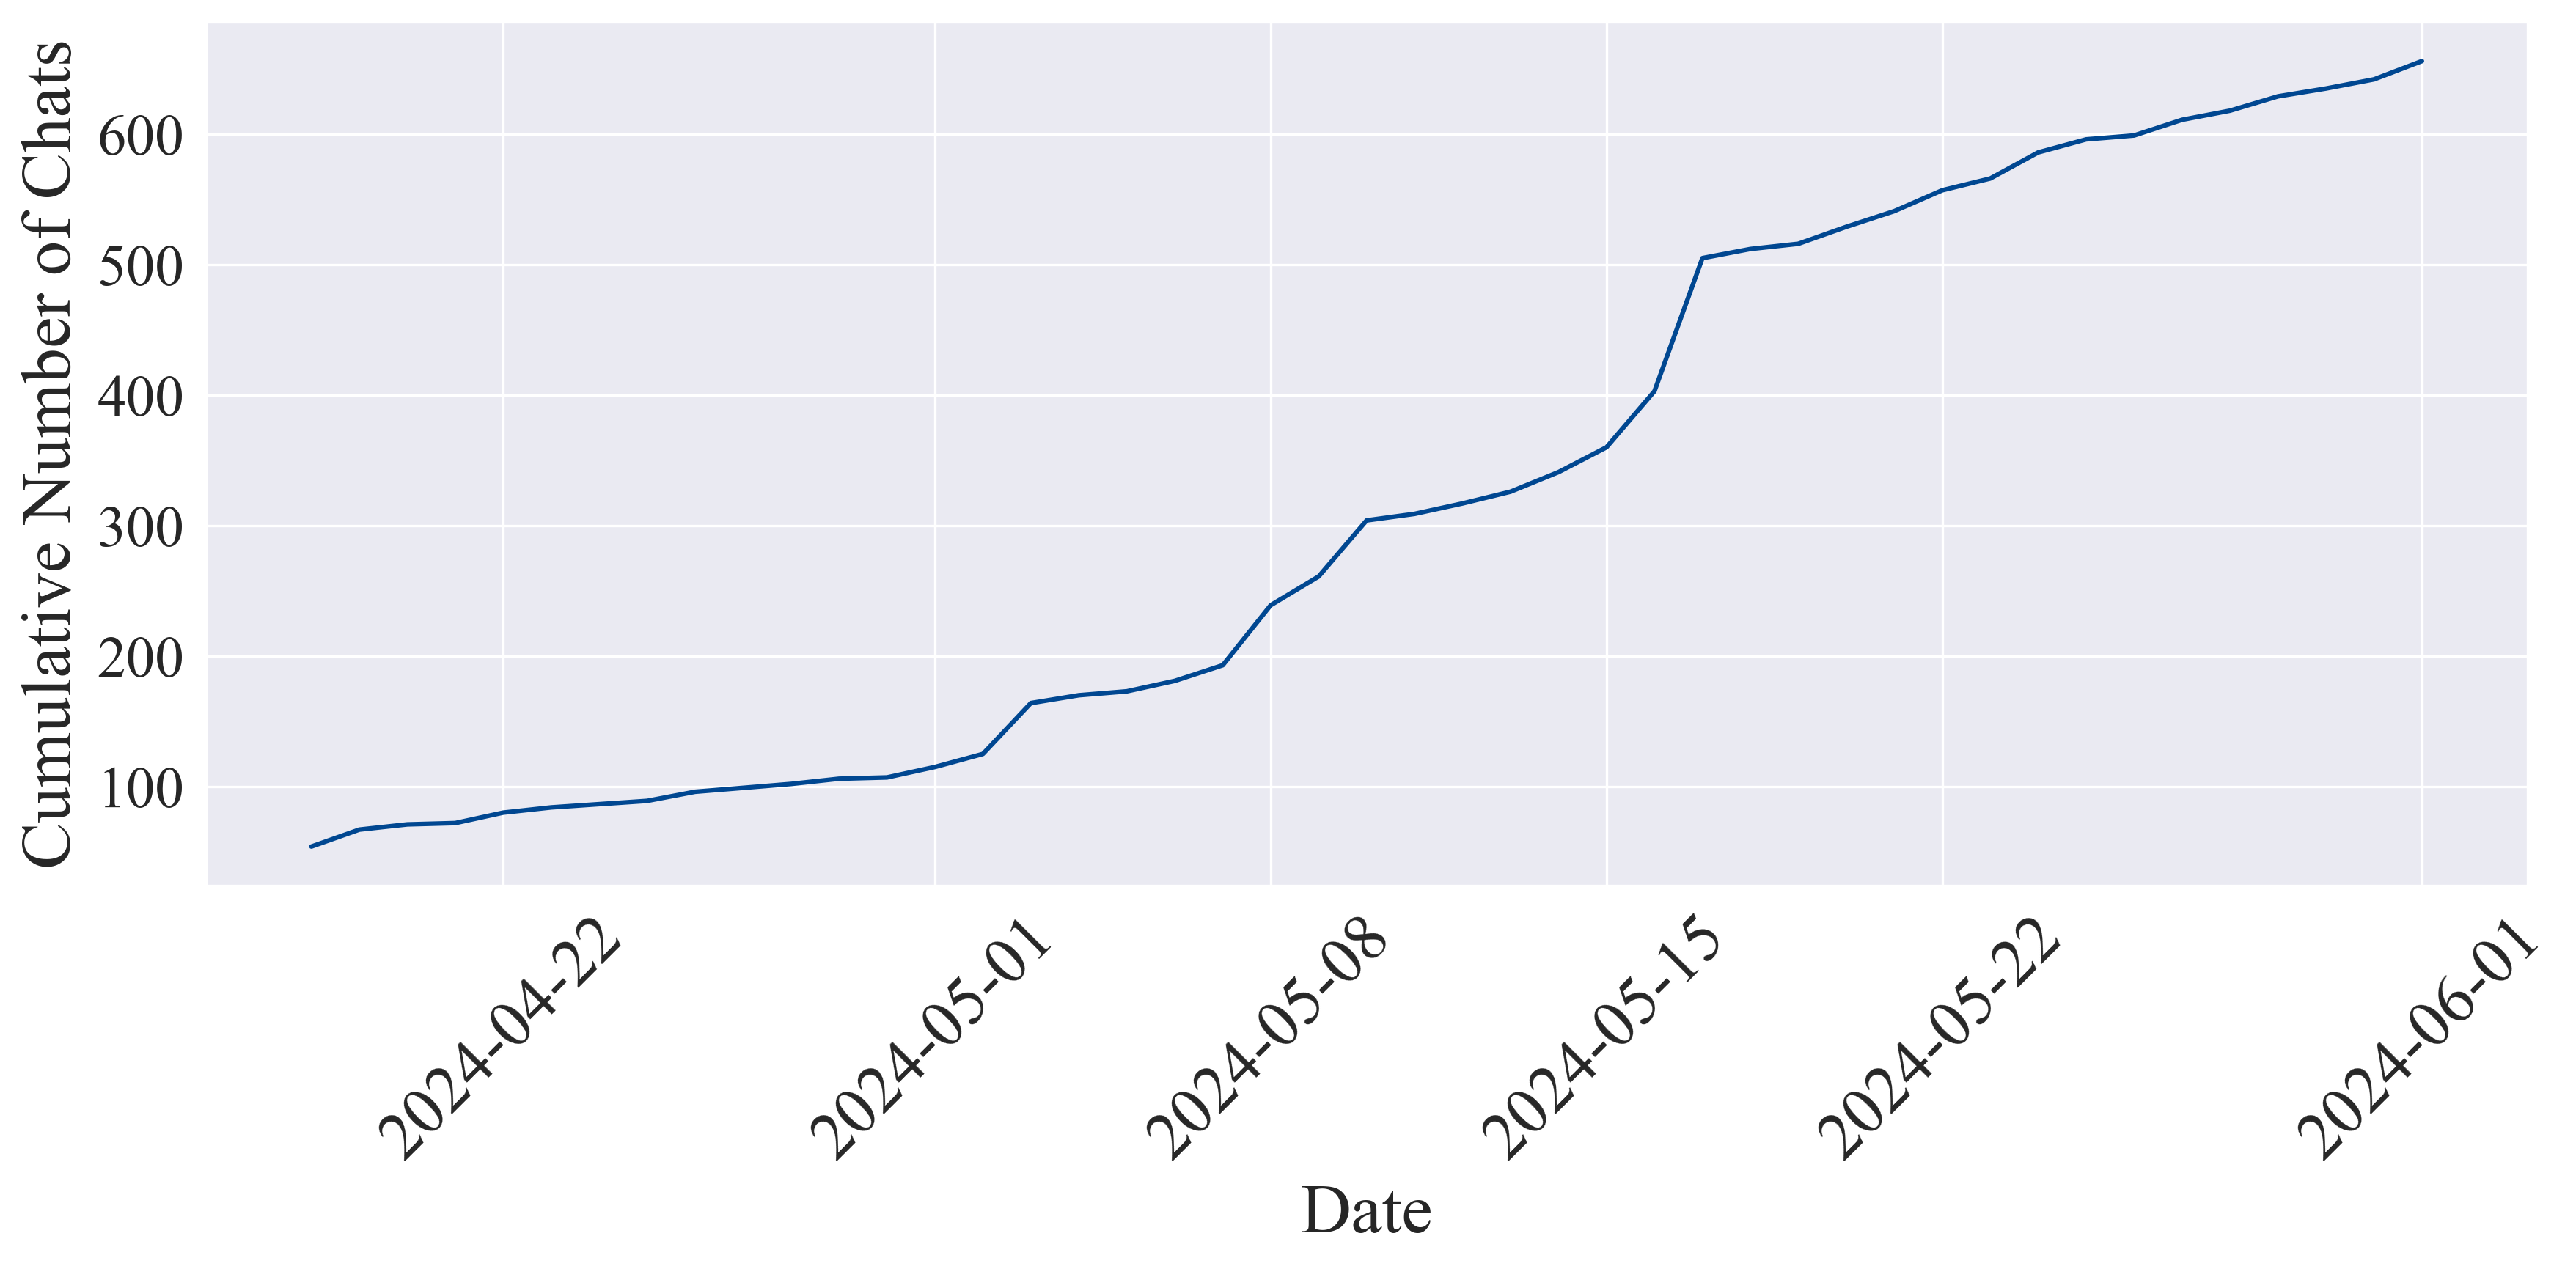
\includegraphics[width=1\textwidth]{results/plots/assets/usage-01-cumulative-number-of-chats.png}
    \caption{Cumulative number of chats started by users participating in the study}
    \label{fig:usage_01_cumulative_number_of_chats}
\end{figure}


\begin{figure}[H]
    \centering
    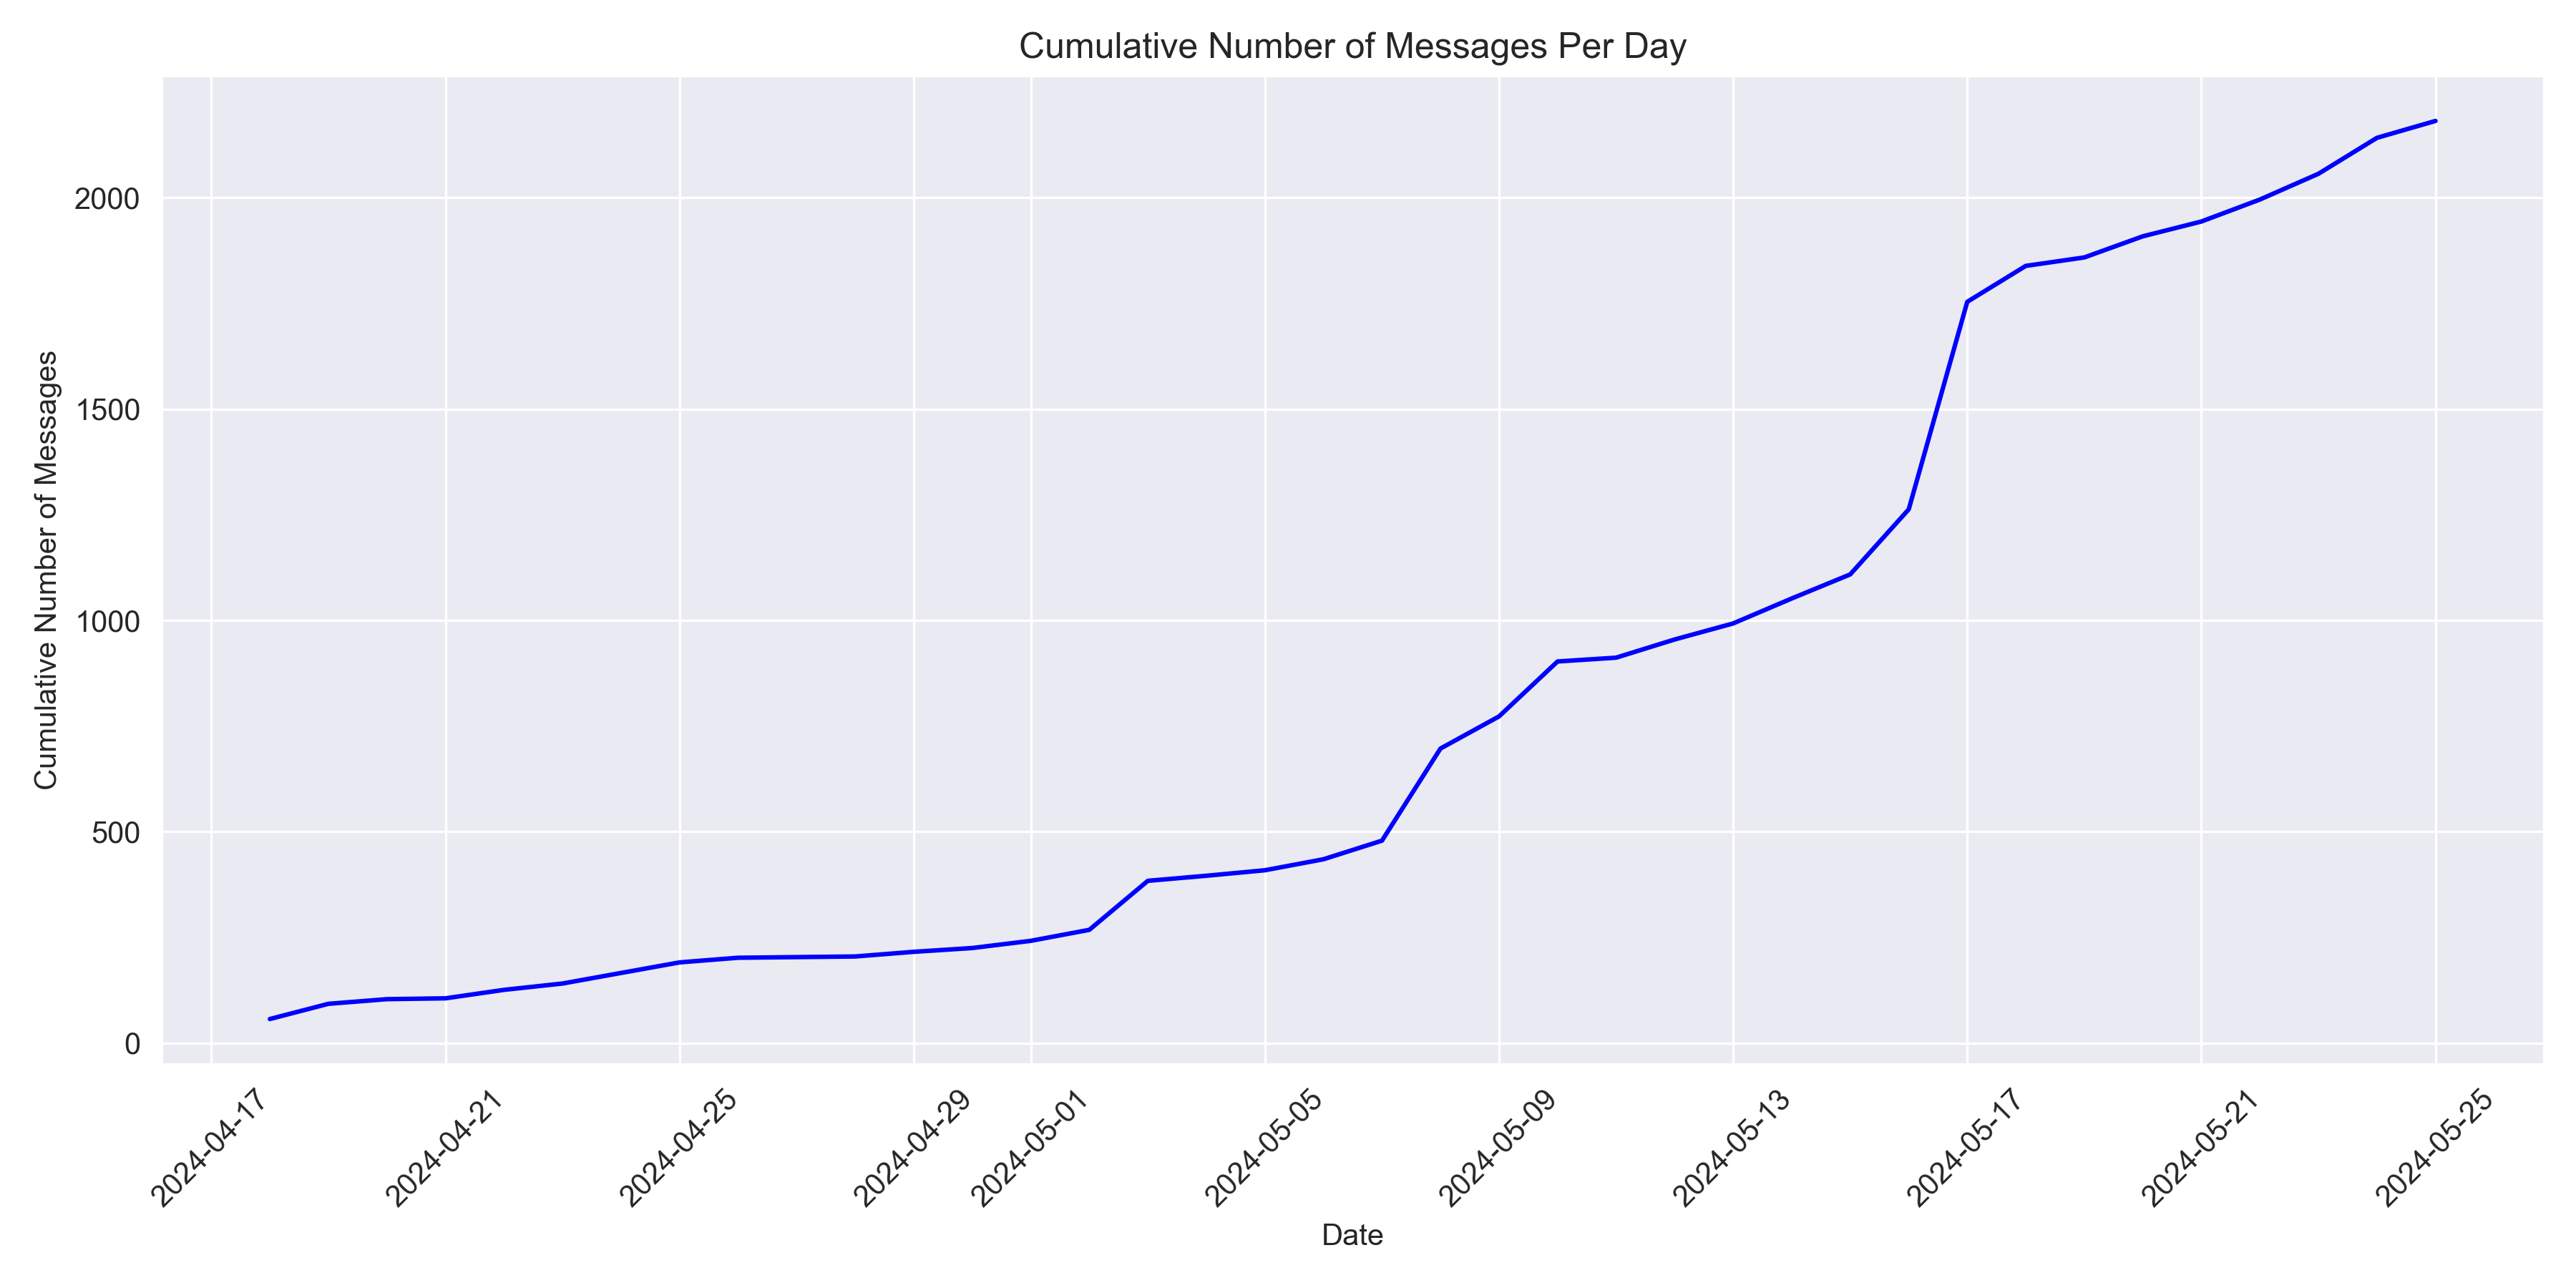
\includegraphics[width=1\textwidth]{results/plots/assets/usage-08-number-of-messages-per-day.png}
    \caption{Cumulative number of messages per day}
    \label{fig:usage_08_number_of_messages_per_day}
\end{figure}


Separating the chats initiated in the separate course rooms we observe that some courses followed a fairly linear increase in the number of chats. One example of this is the course \textit{MG2040 Assembly Technology 6.0 credits}, which can be seen in figure~\ref{fig:usage_02_cumulative_number_of_chats_per_course}.


\begin{figure}[H]
    \centering
    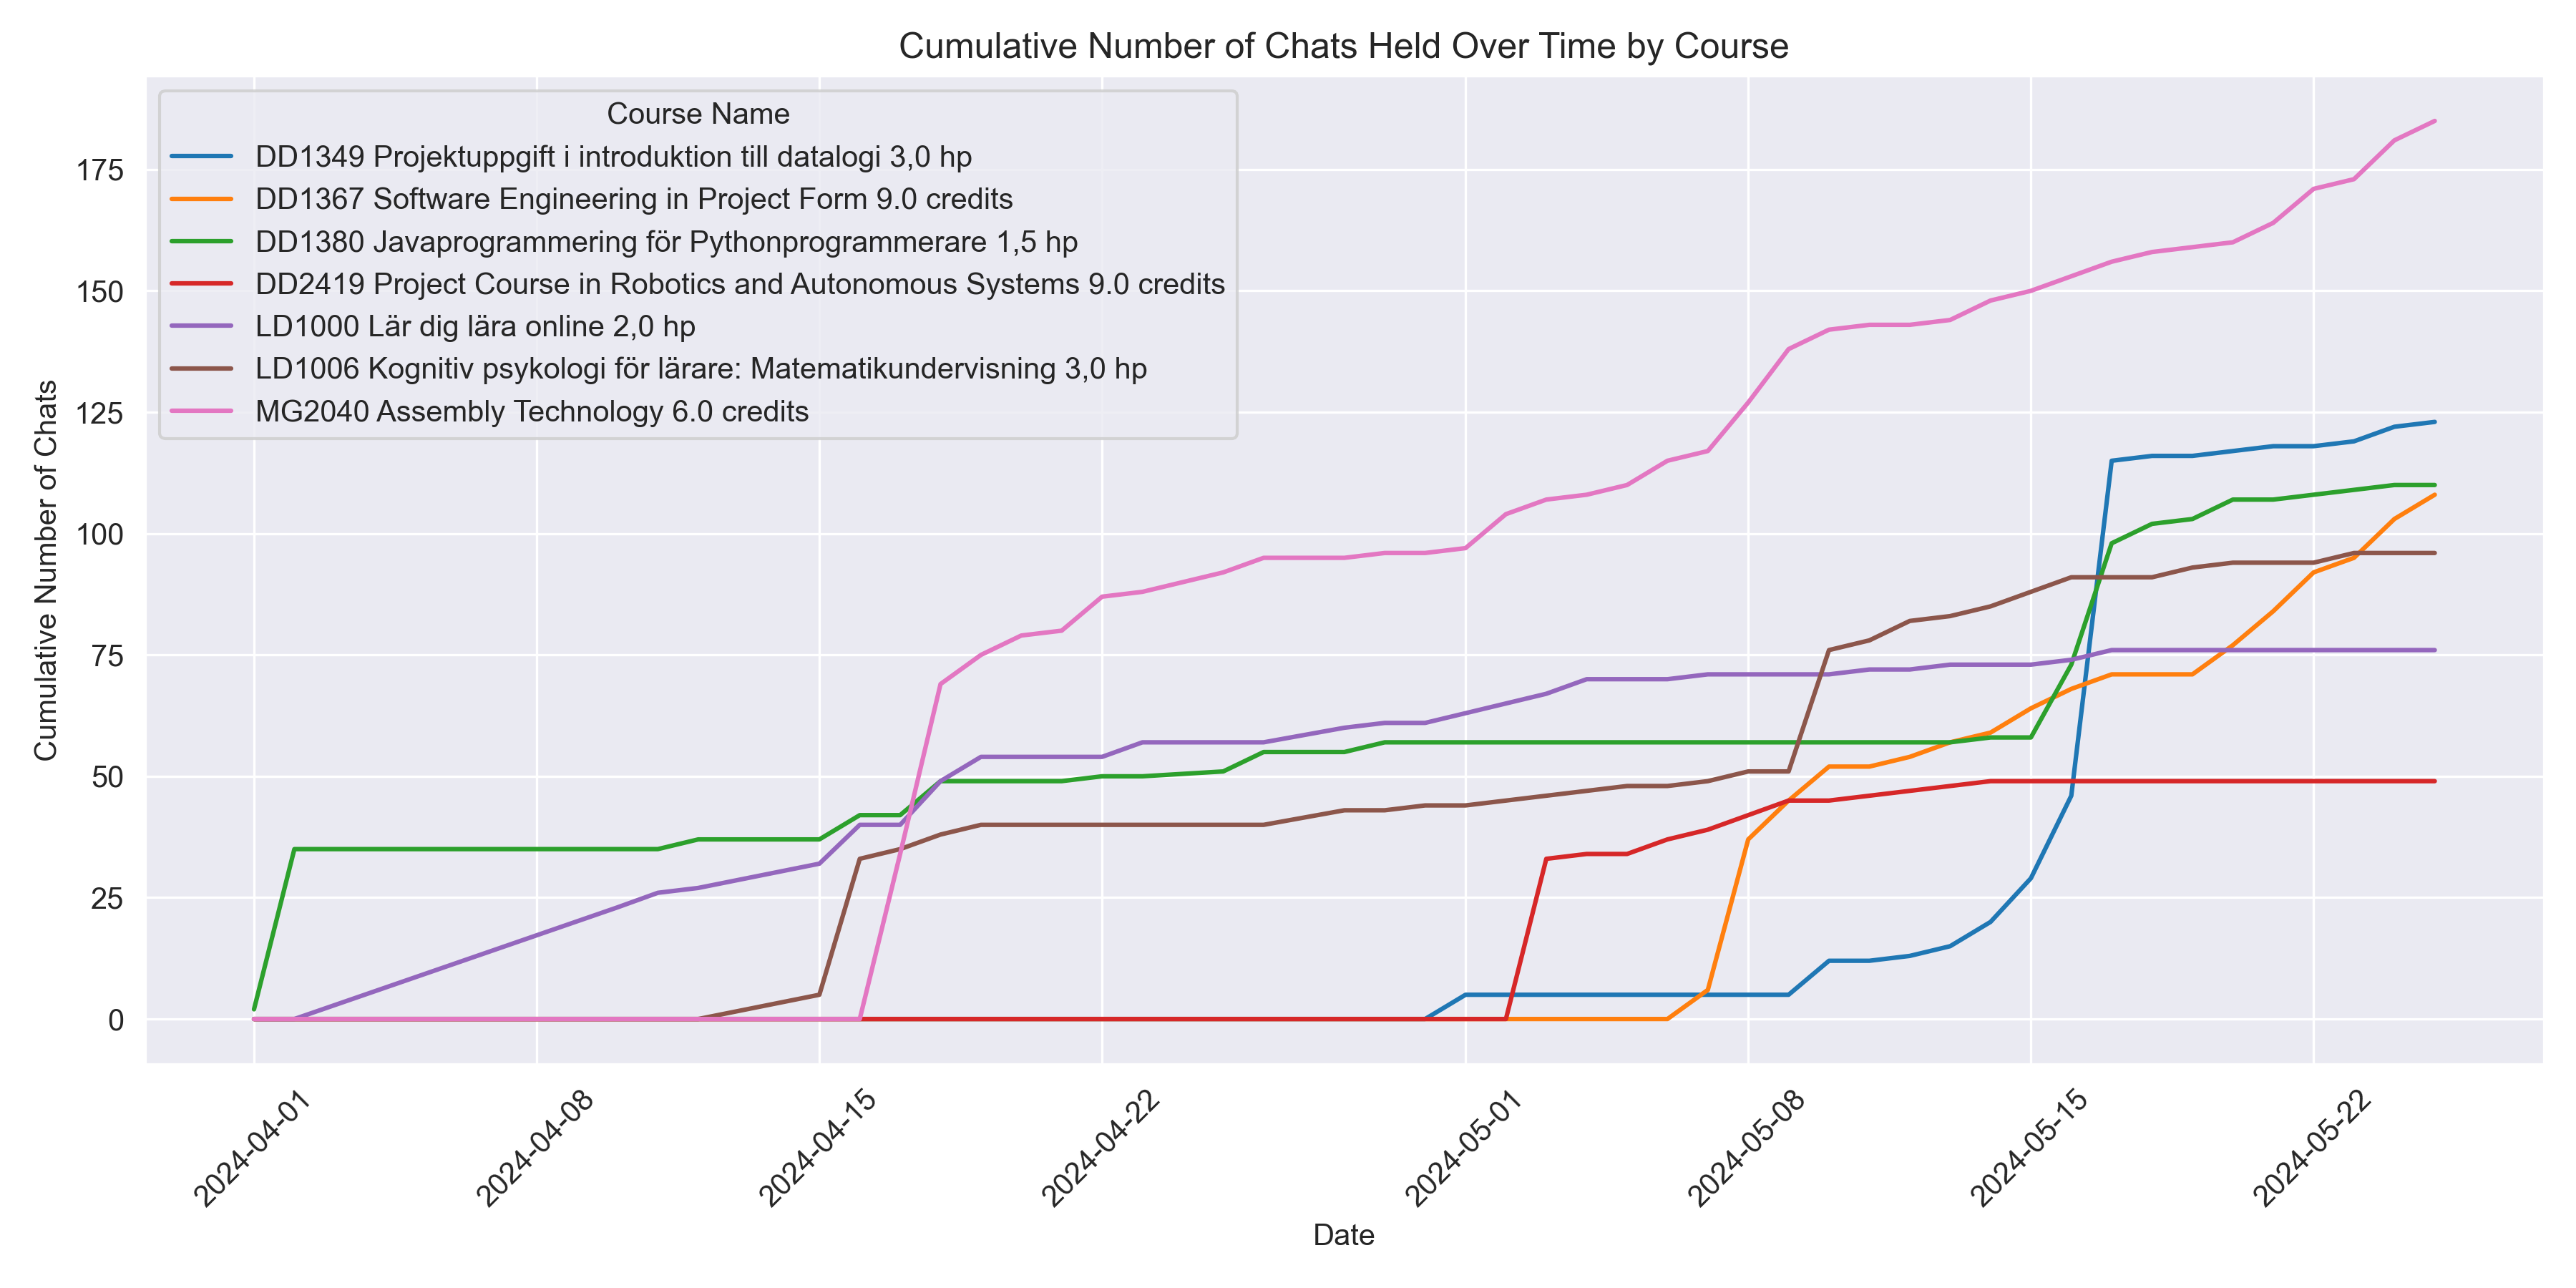
\includegraphics[width=\textwidth]{results/plots/assets/usage-02-cumulative-number-of-chats-per-course.png}
    \caption{Cumulative number of chats started by users participating in the study in each course}
    \label{fig:usage_02_cumulative_number_of_chats_per_course}
\end{figure}


Looking at other courses in figure~\ref{fig:usage_02_cumulative_number_of_chats_per_course} it is evident that not all courses follow the same pattern as \textit{MG2040}. Some courses initially have very few chats due to the chatbot not being deployed simultaneously across all courses. \autoref{tab:course_start_dates} details the start dates for each course. For instance, \textit{DD1349 Projektuppgift i introduktion till datalogi 3,0 hp} exhibits a steep increase in users when it launched, followed by no further growth. This is because the course officially ended shortly after the chatbot was introduced. In all courses participating in the study, the chatbot was deployed well after the courses had already begun, therefore a similar pattern can be seen in many other courses.


\begin{table}[H]
\centering
{\scriptsize
\begin{tabularx}{\textwidth}{@{}X c@{}}
\toprule
\textbf{Course} & \textbf{Go live date} \\ \midrule
LD1000 Lär dig lära online 2,0 hp & 2024-04-17 \\
LD1006 Kognitiv psykologi för lärare: Matematikundervisning 3,0 hp & 2024-04-17 \\
MG2040 Assembly Technology 6.0 credits & 2024-04-17 \\
DD1349 Projektuppgift i introduktion till datalogi 3,0 hp & 2024-05-01 \\
DD2419 Project Course in Robotics and Autonomous Systems 9.0 credits & 2024-05-03 \\
DD1367 Software Engineering in Project Form 9.0 credits & 2024-05-07 \\
DD1380 Javaprogrammering för Pythonprogrammerare 1,5 hp & 2024-05-13 \\
\bottomrule
\end{tabularx}
}
\vspace{2mm}
\caption{The start dates for each course, when the bot was deployed in each canvas course room.}
\label{tab:course_start_dates}
\end{table}



\autoref{fig:usage_03_number_of_chats_per_course} shows the total number of chats held in each course, and \autoref{fig:usage_03_number_of_chats_per_calendar_week_per_course} shows how these were distributed over each course over time. The course \textit{MG2040} held the most, 151chats. \textit{DD1349} held the second most and \textit{DD1367} the third most, 123and 122chats respectively.


\begin{figure}[H]
    \centering
    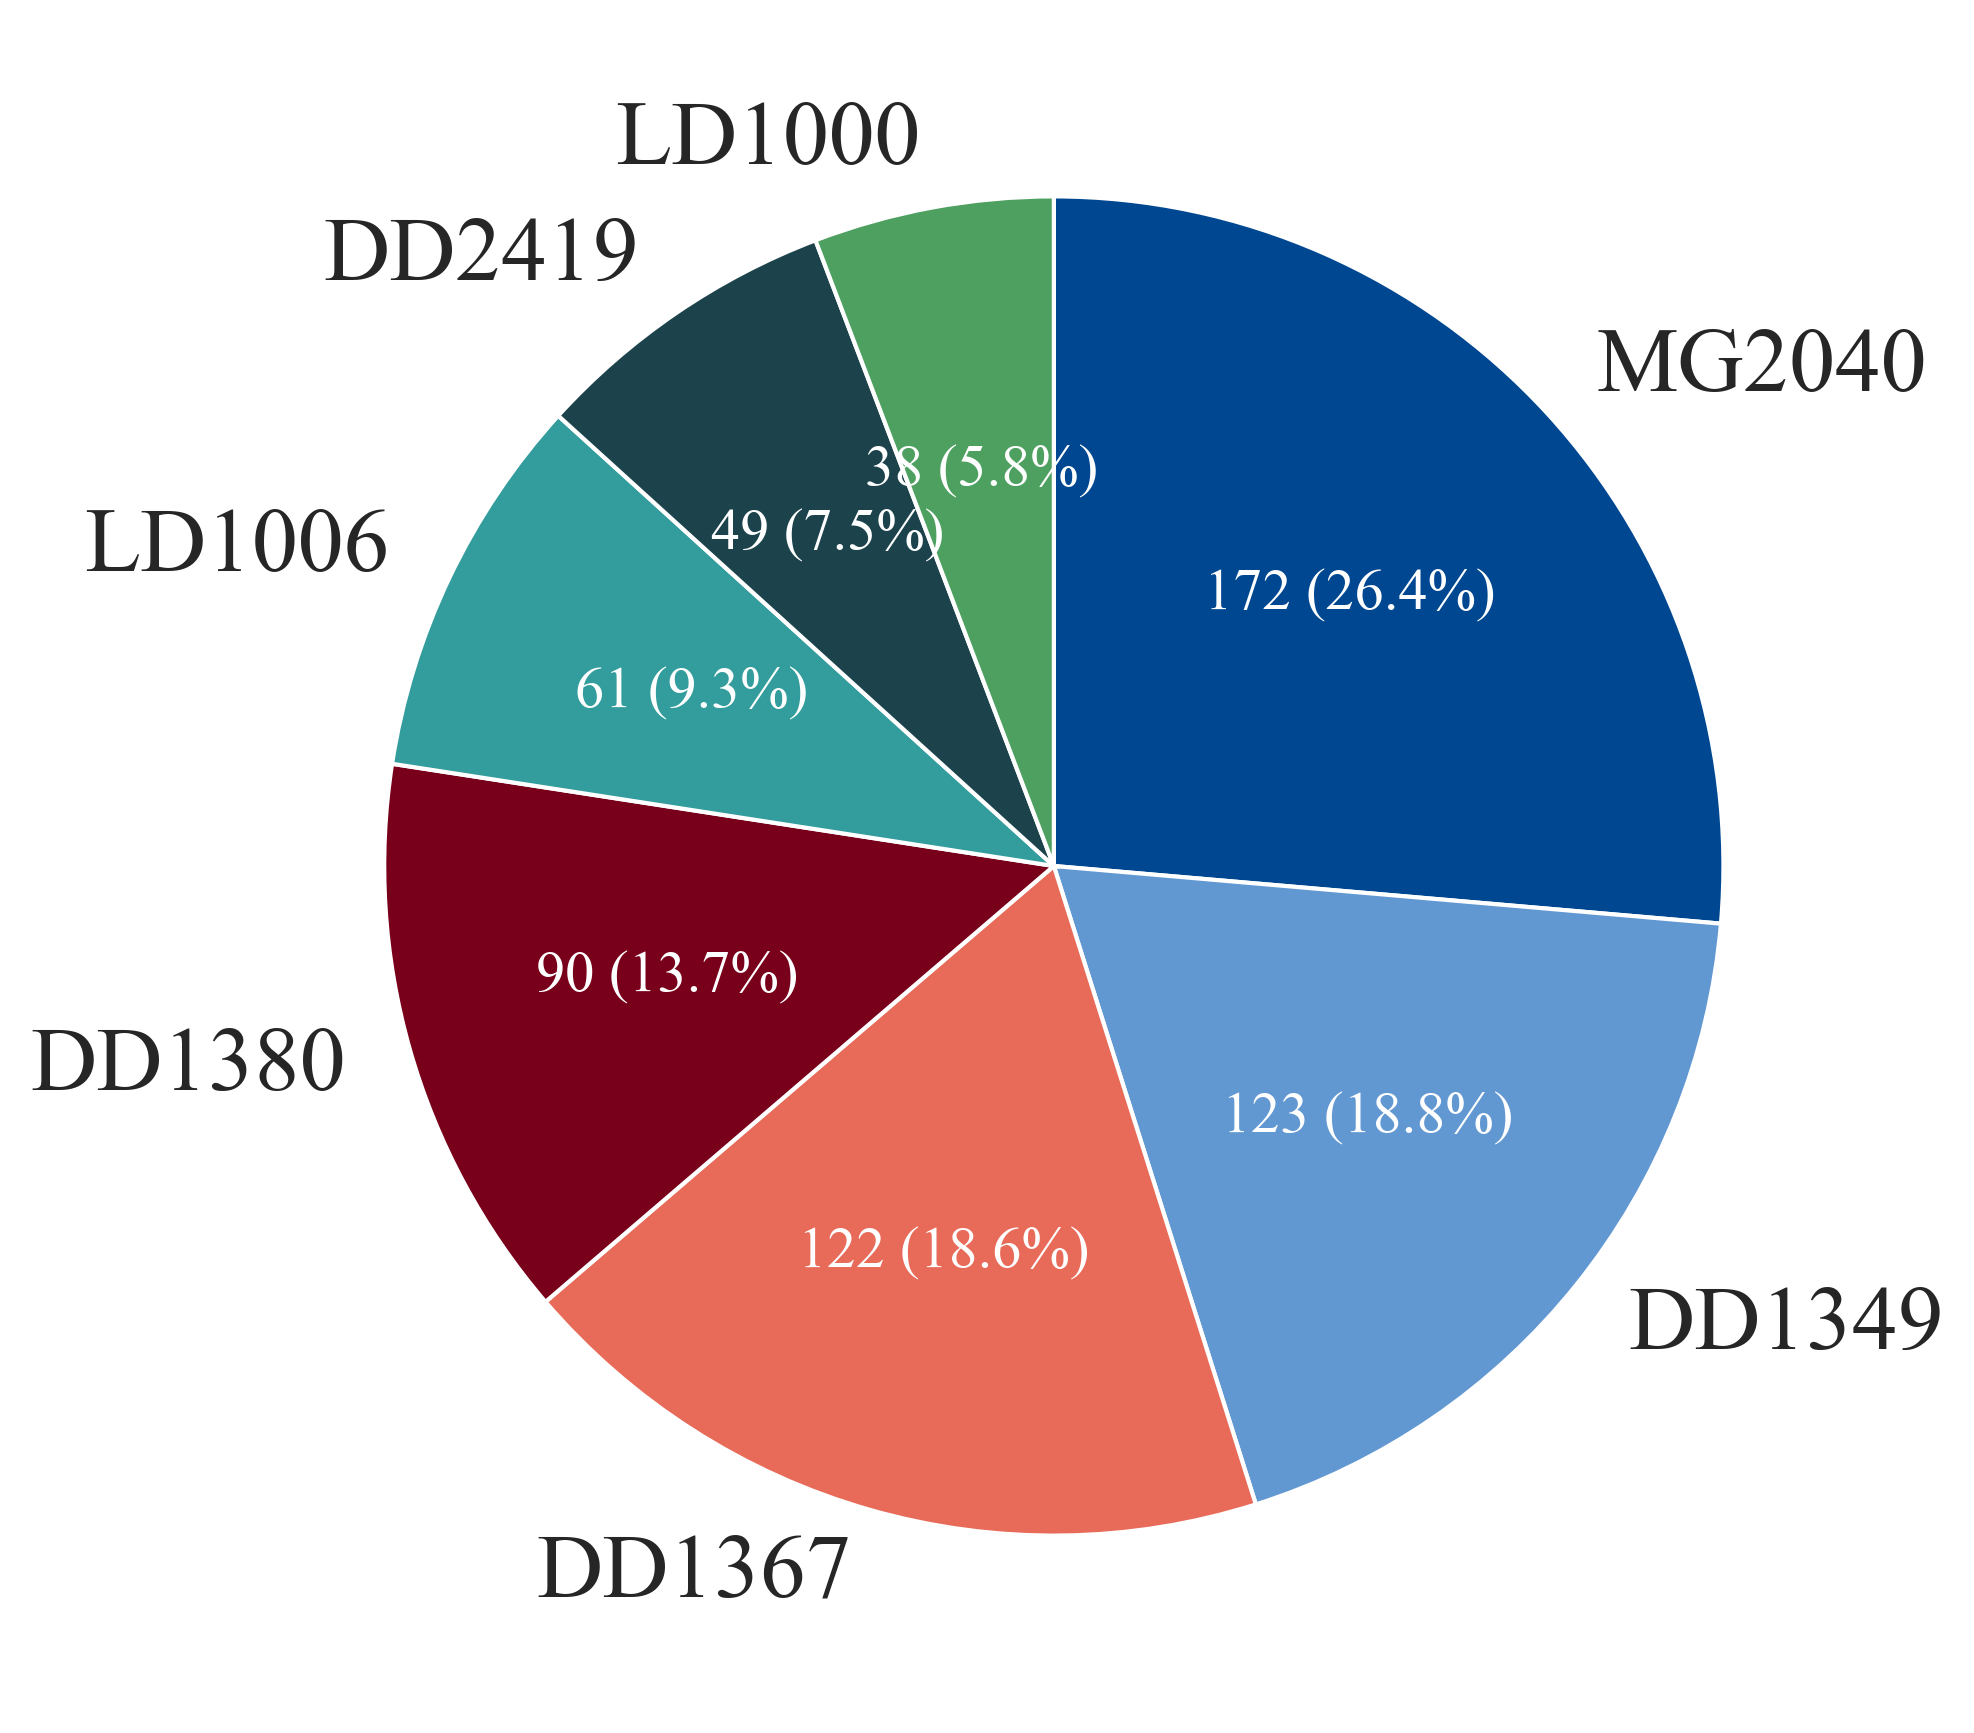
\includegraphics[width=\textwidth]{results/plots/assets/usage-05-number-of-chats-per-course.png}
    \caption{Number of chats held by in each course}
    \label{fig:usage_03_number_of_chats_per_course}
\end{figure}


\begin{figure}[H]
    \centering
    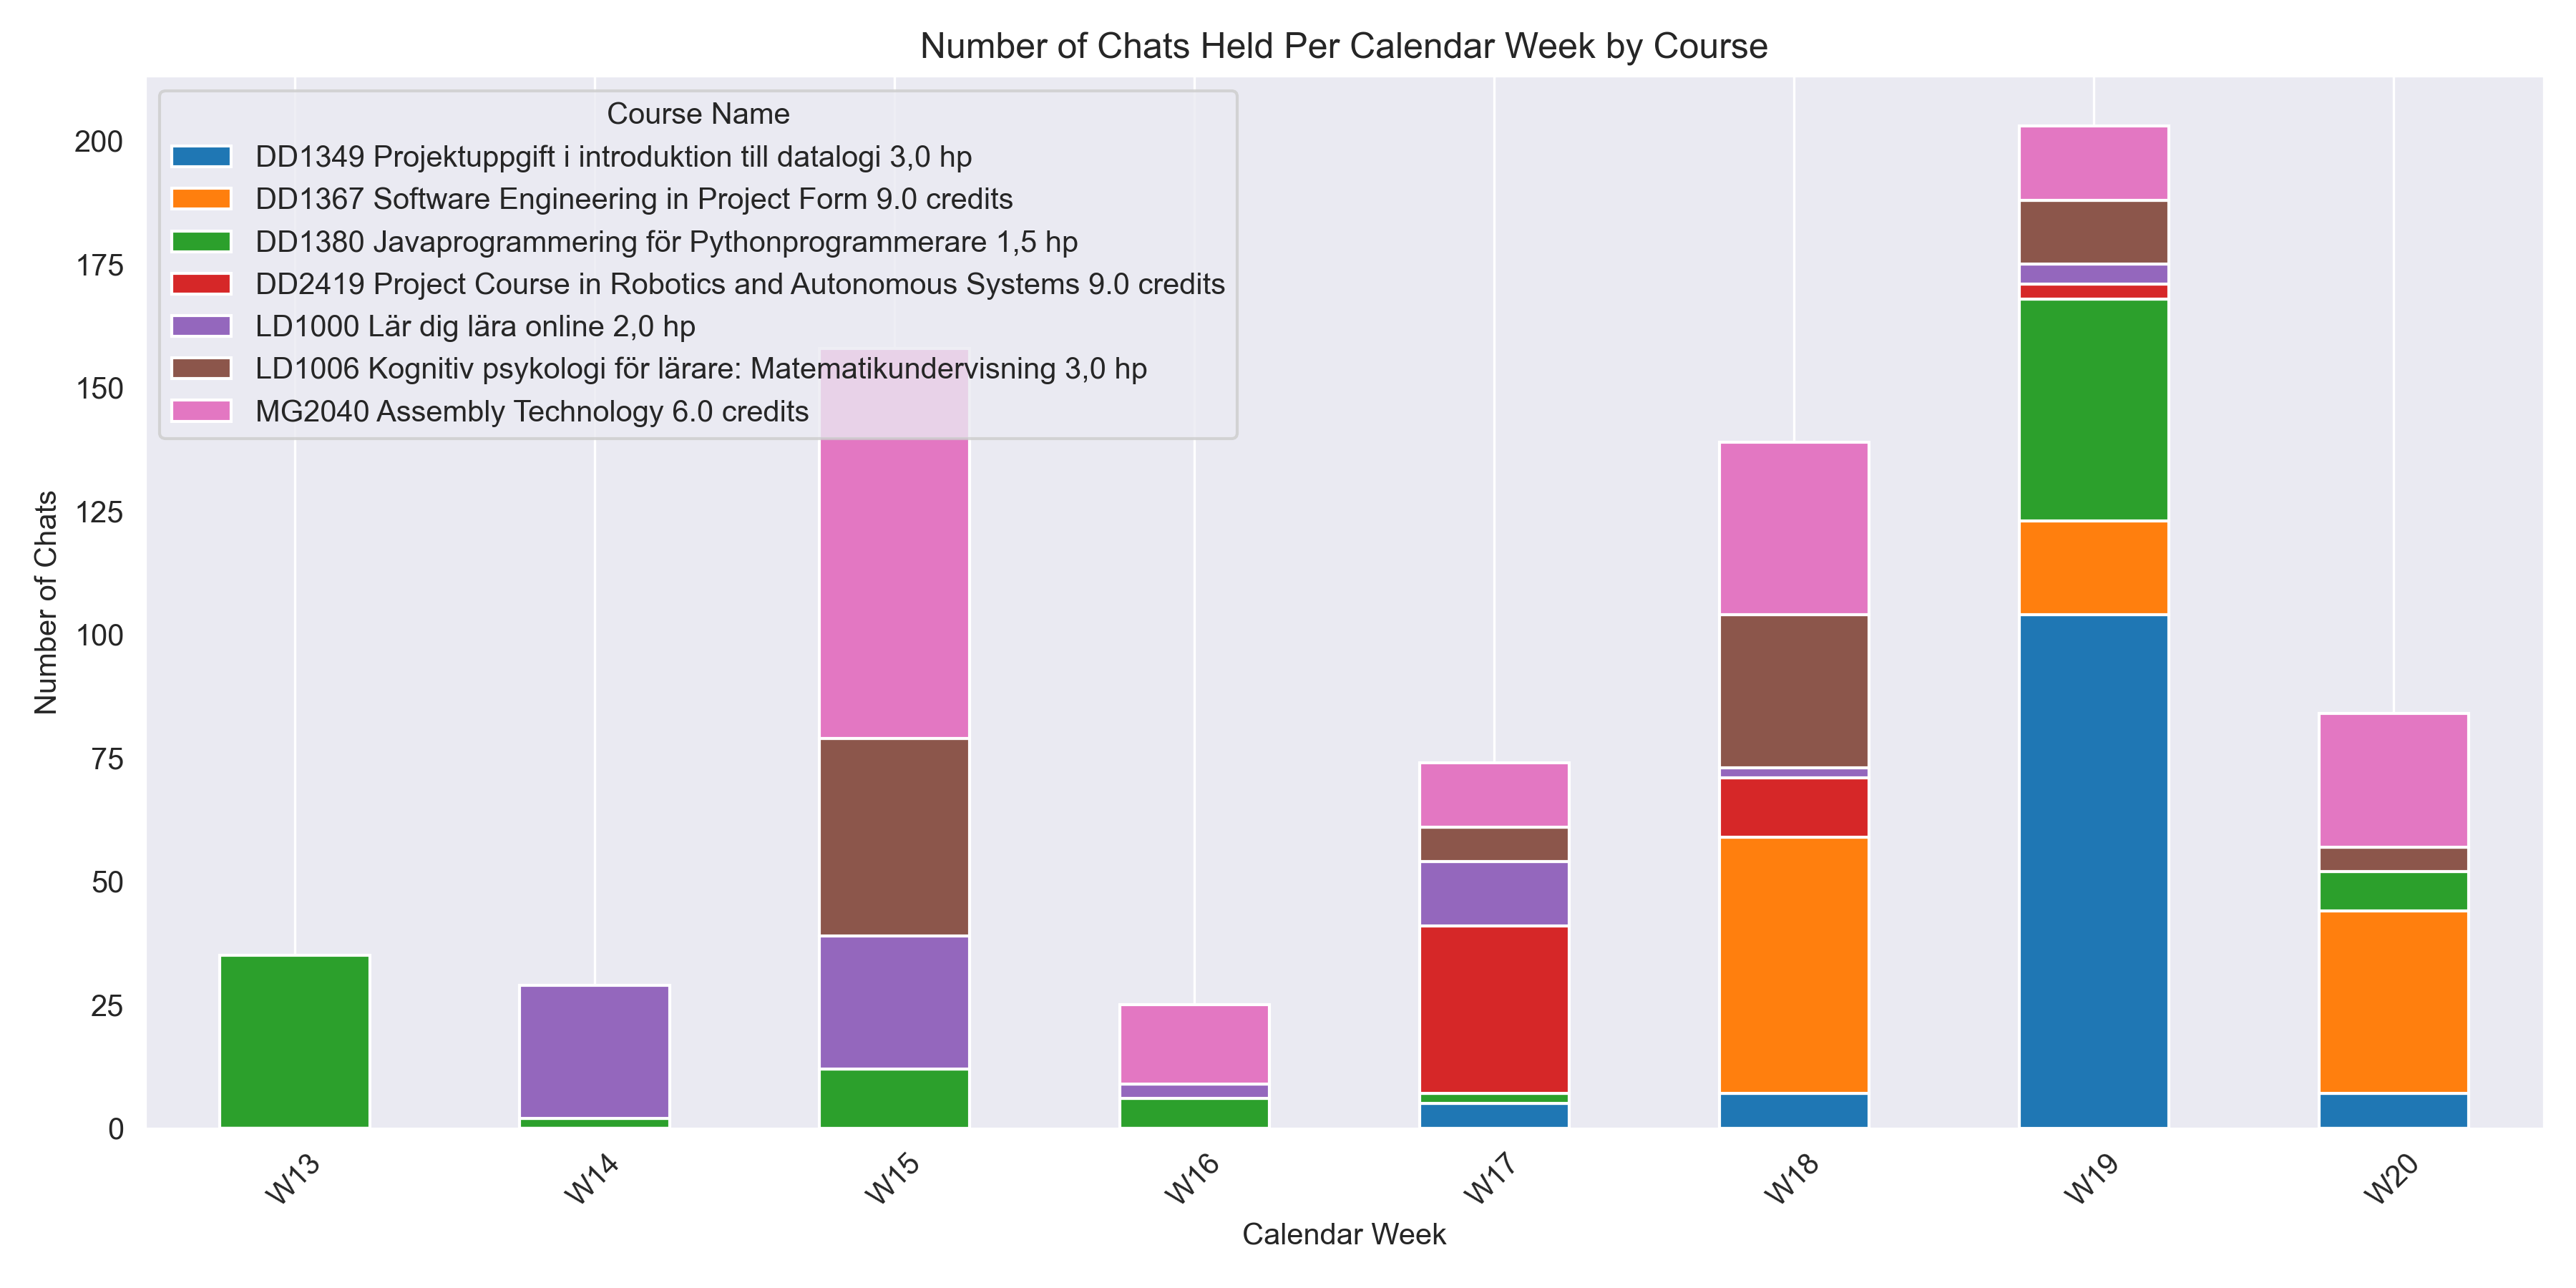
\includegraphics[width=\textwidth]{results/plots/assets/usage-04-number-of-chats-per-calendar-week-per-course.png}
    \caption{Number of chats held each week per course}
    \label{fig:usage_03_number_of_chats_per_calendar_week_per_course}
\end{figure}




Looking at the number of sessions created in \autoref{fig:usage_06_number_of_sessions_per_day} and \autoref{fig:usage_07_number_of_sessions_per_day_and_course}, we can see a similar pattern linear pattern. A session is started whenever a user loads the application without already having loaded it before. A session is not tracked between devices, therefore a user would have two sessions if the same user accessed the chat on two different devices, such as a desktop and a mobile phone. However, the same session is used across courses.


\begin{figure}[H]
    \centering
    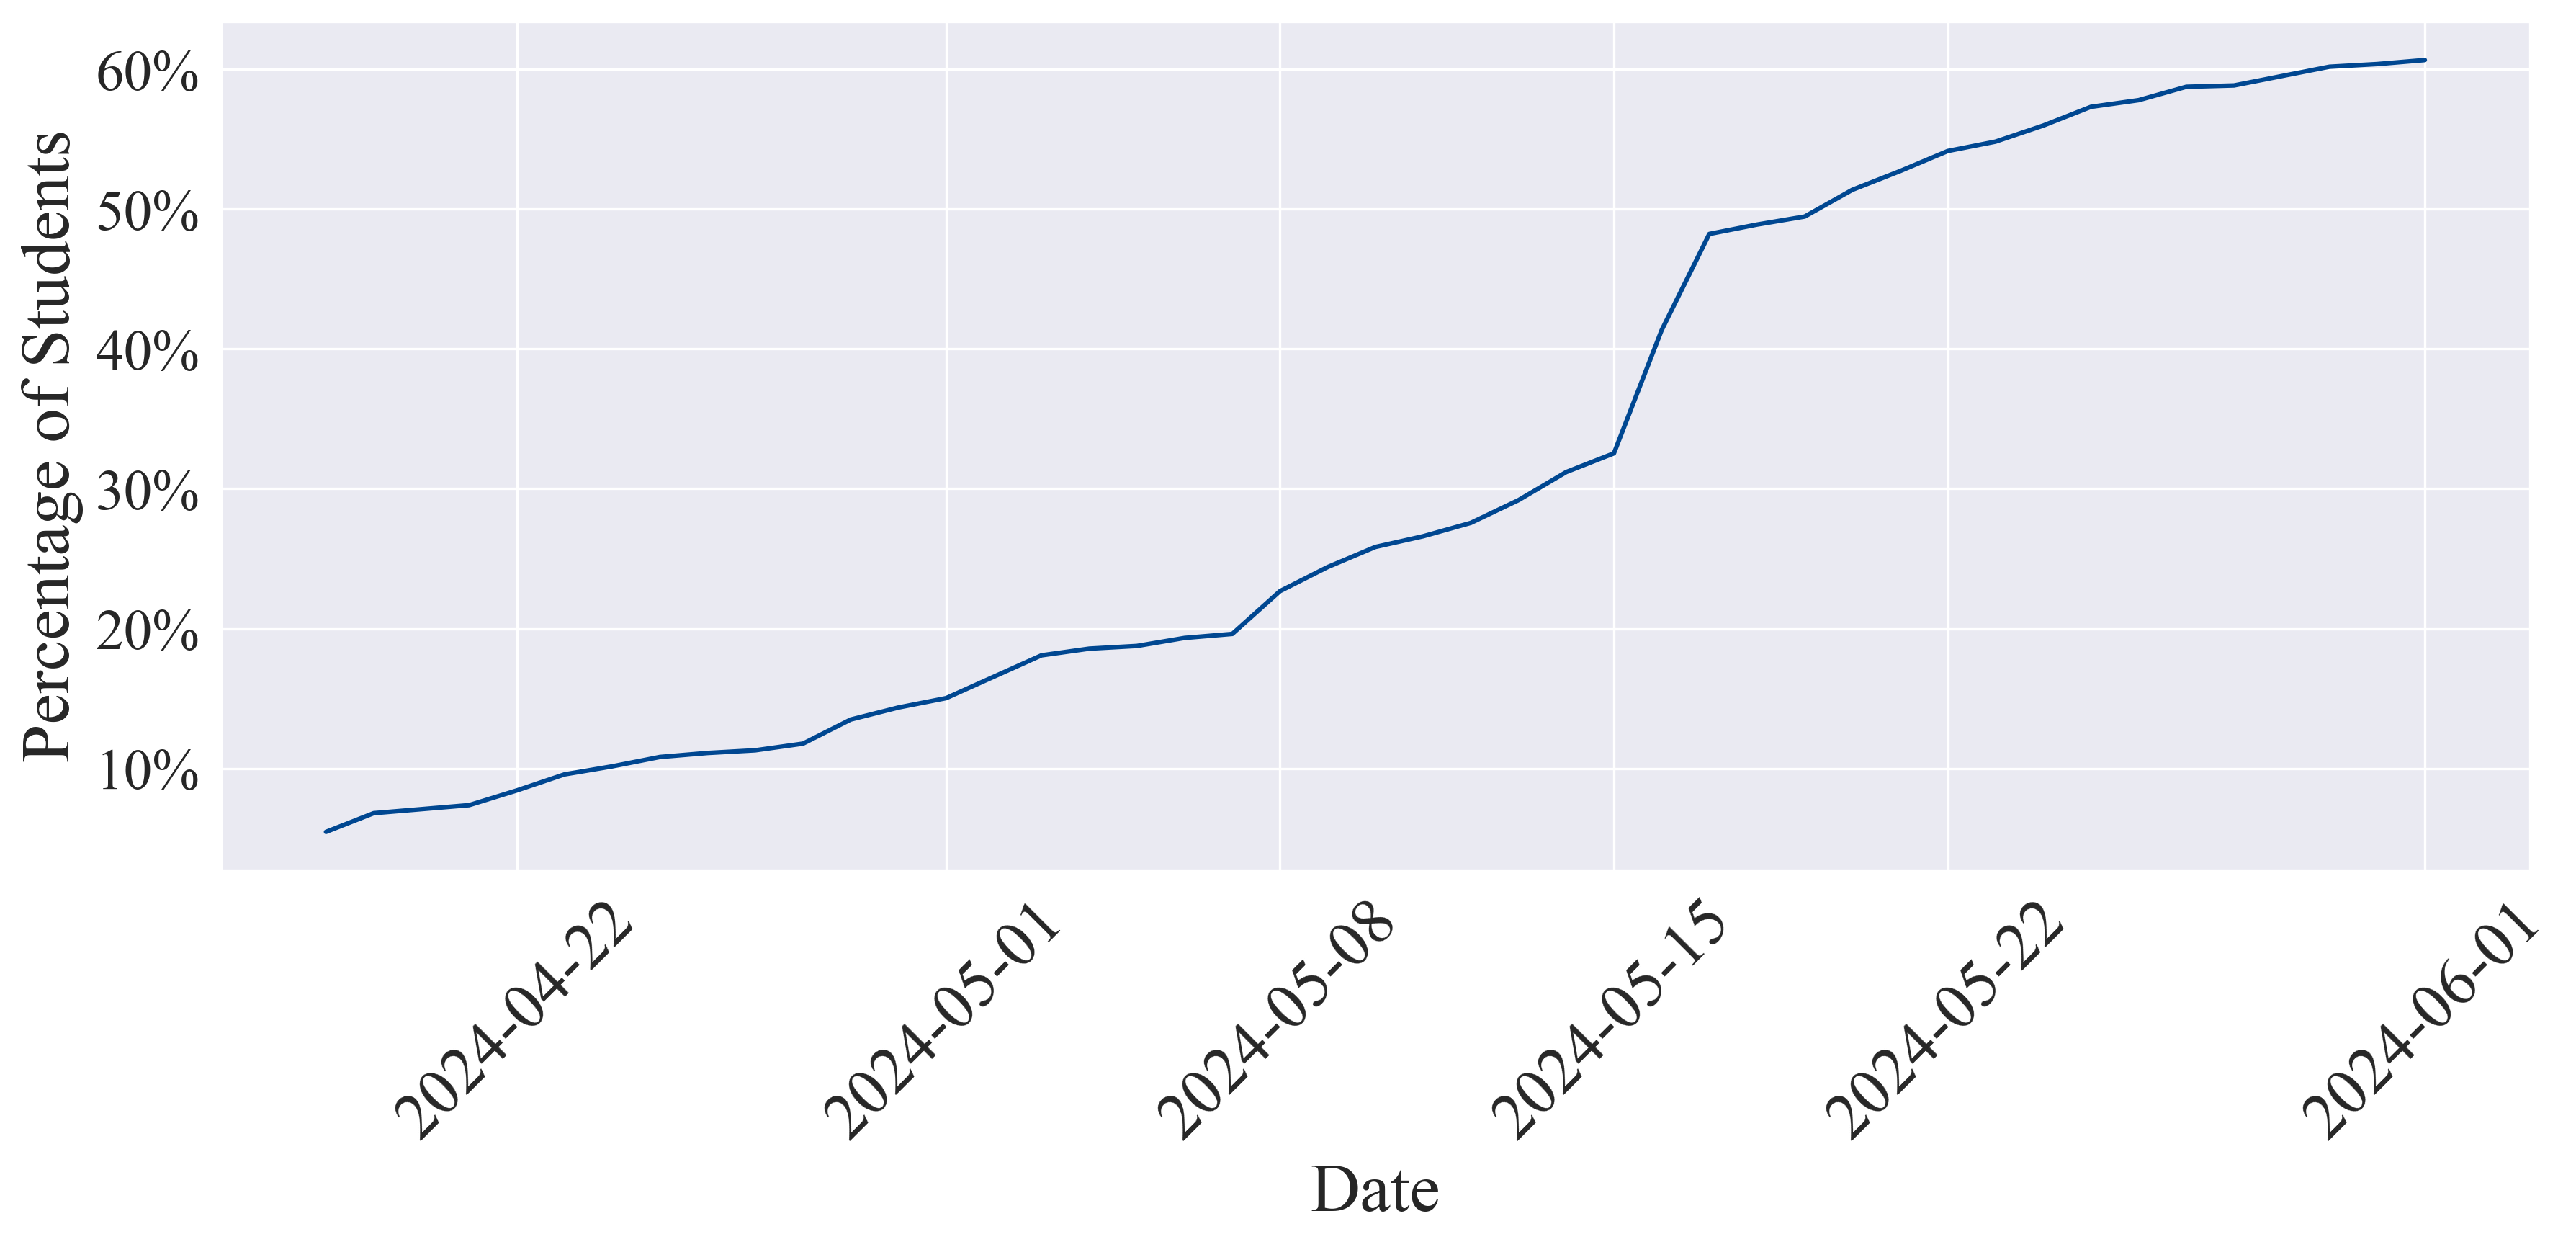
\includegraphics[width=\textwidth]{results/plots/assets/usage-06-number-of-sessions-per-day.png}
    \caption{Cumulative number of users as percentage of number of users in all participating courses that had started a chat}
    \label{fig:usage_06_number_of_sessions_per_day}
\end{figure}


\begin{figure}[H]
    \centering
    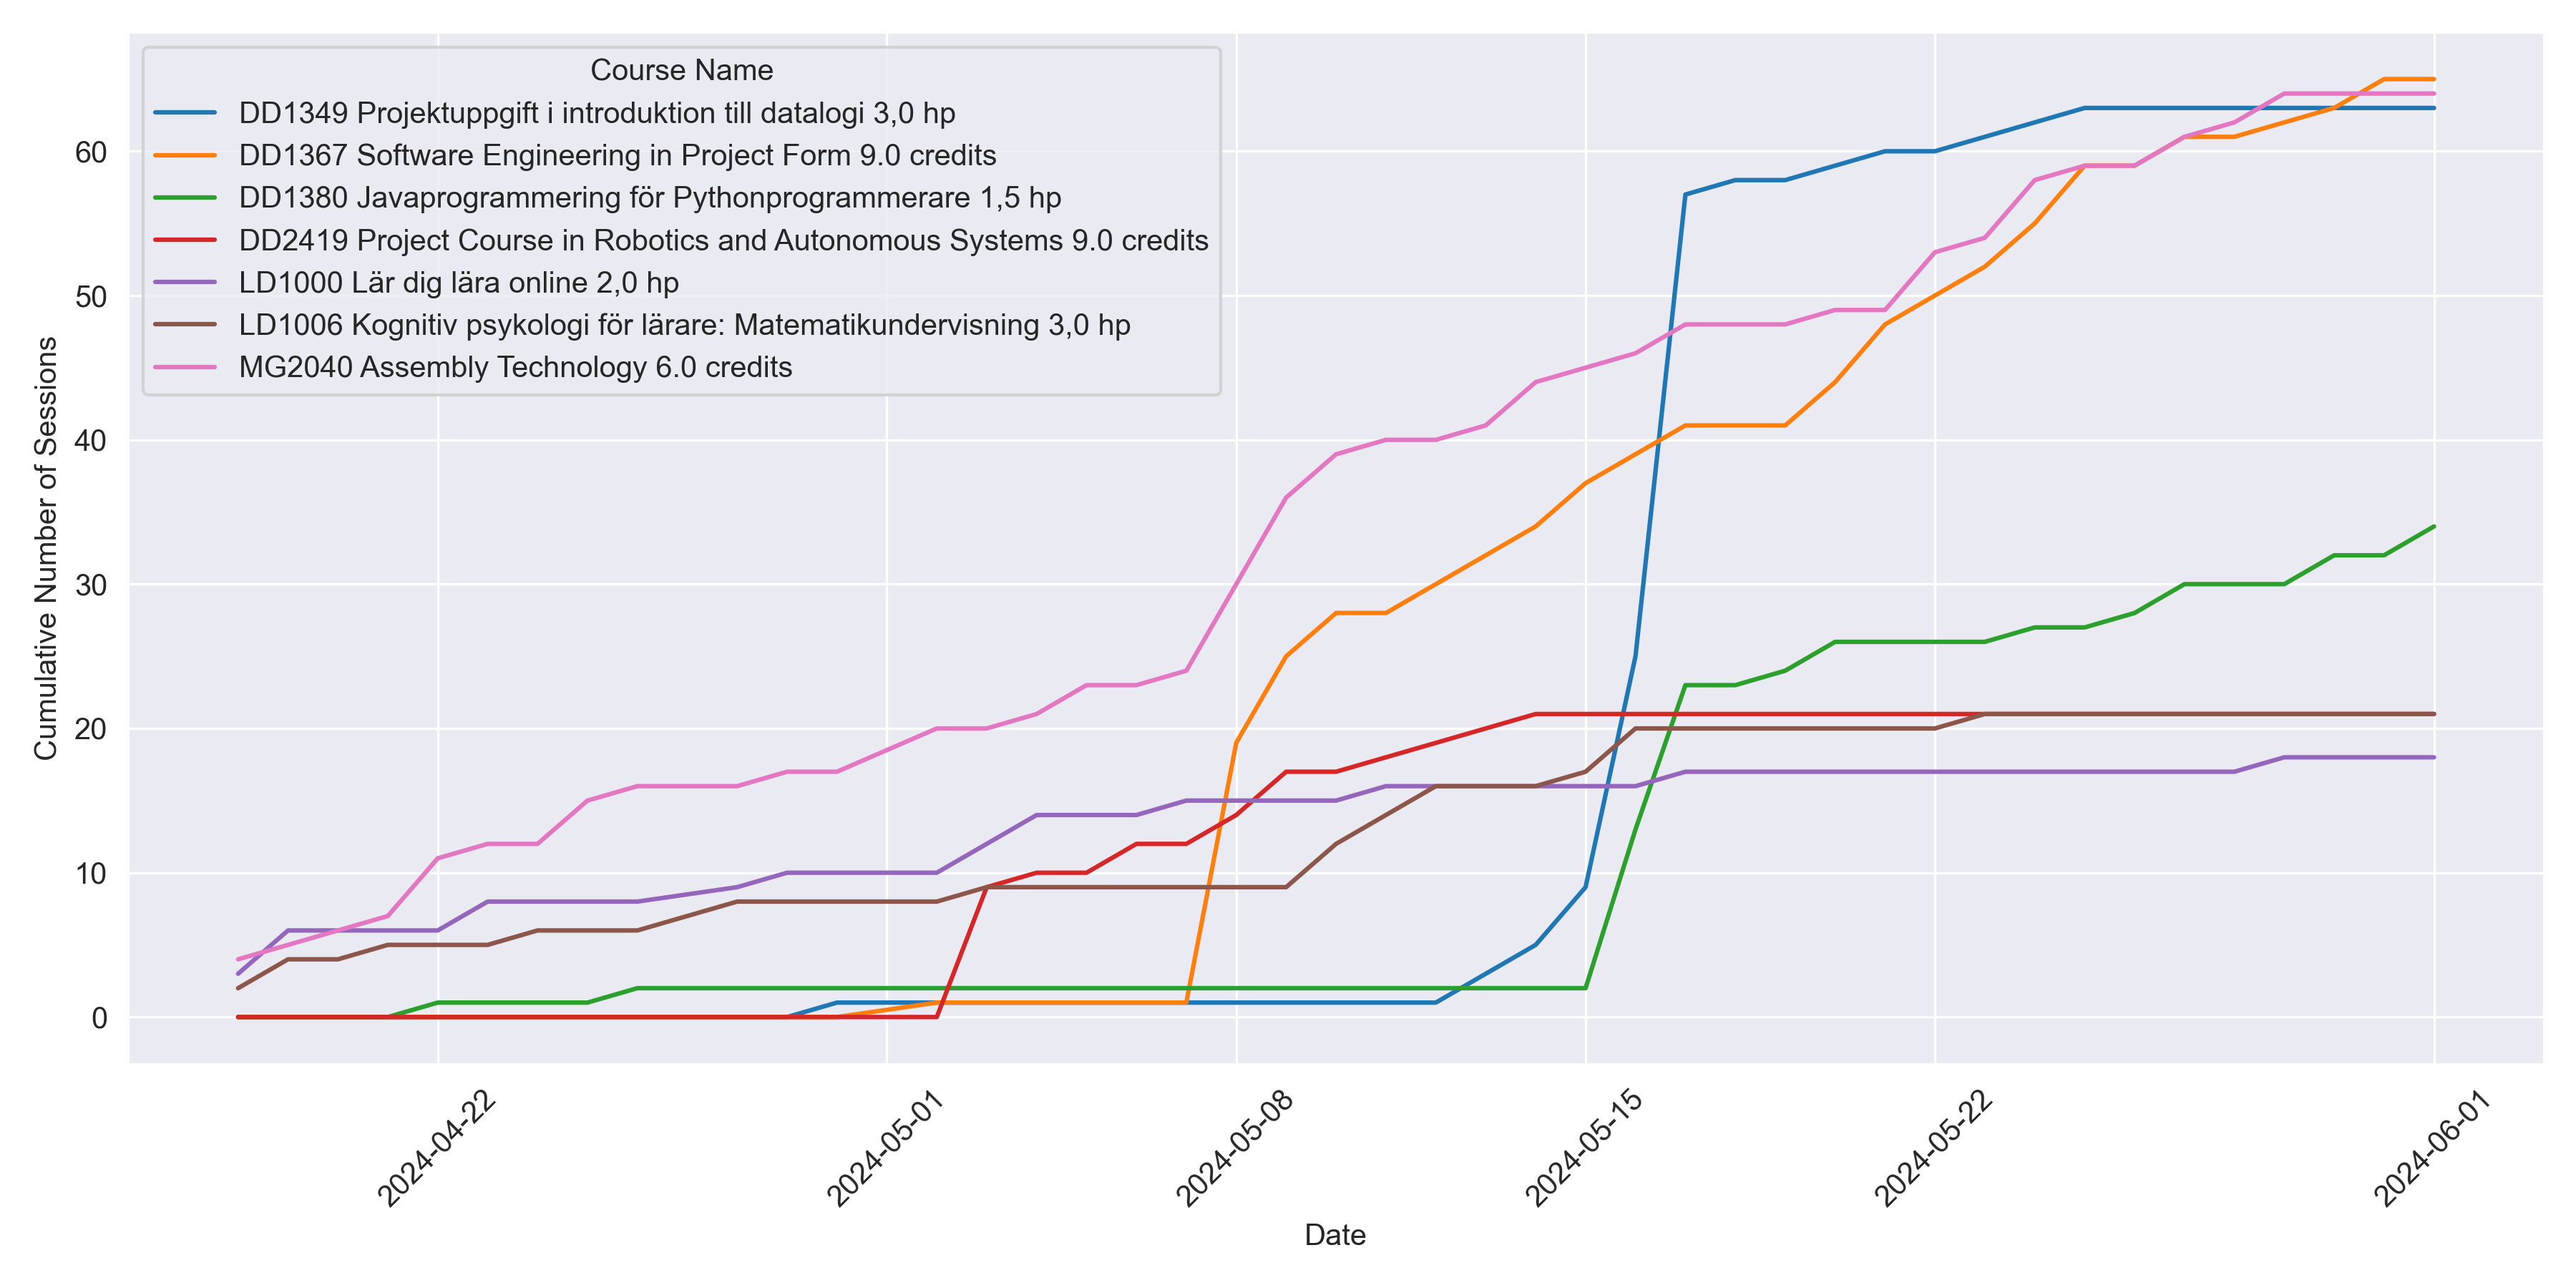
\includegraphics[width=1\textwidth]{results/plots/assets/usage-07-number-of-sessions-per-day-and-course.png}
    \caption{Cumulative number of users per day in each course, as a percentage of the course's students, that had started a chat}
    \label{fig:usage_07_number_of_sessions_per_day_and_course}
\end{figure}


Looking at the distribution of how many chats and messages is sent per session, as seen in figure \autoref{fig:usage_12_number_of_sessions_with_number_of_chats} and \autoref{fig:usage_13_number_of_sessions_with_number_of_messages} we can see that it was very common for users to only start one or two chats. Most users sent quite a few messages though. The average user held 2.22chats and sent 9.57messages.


\begin{figure}[H]
    \centering
    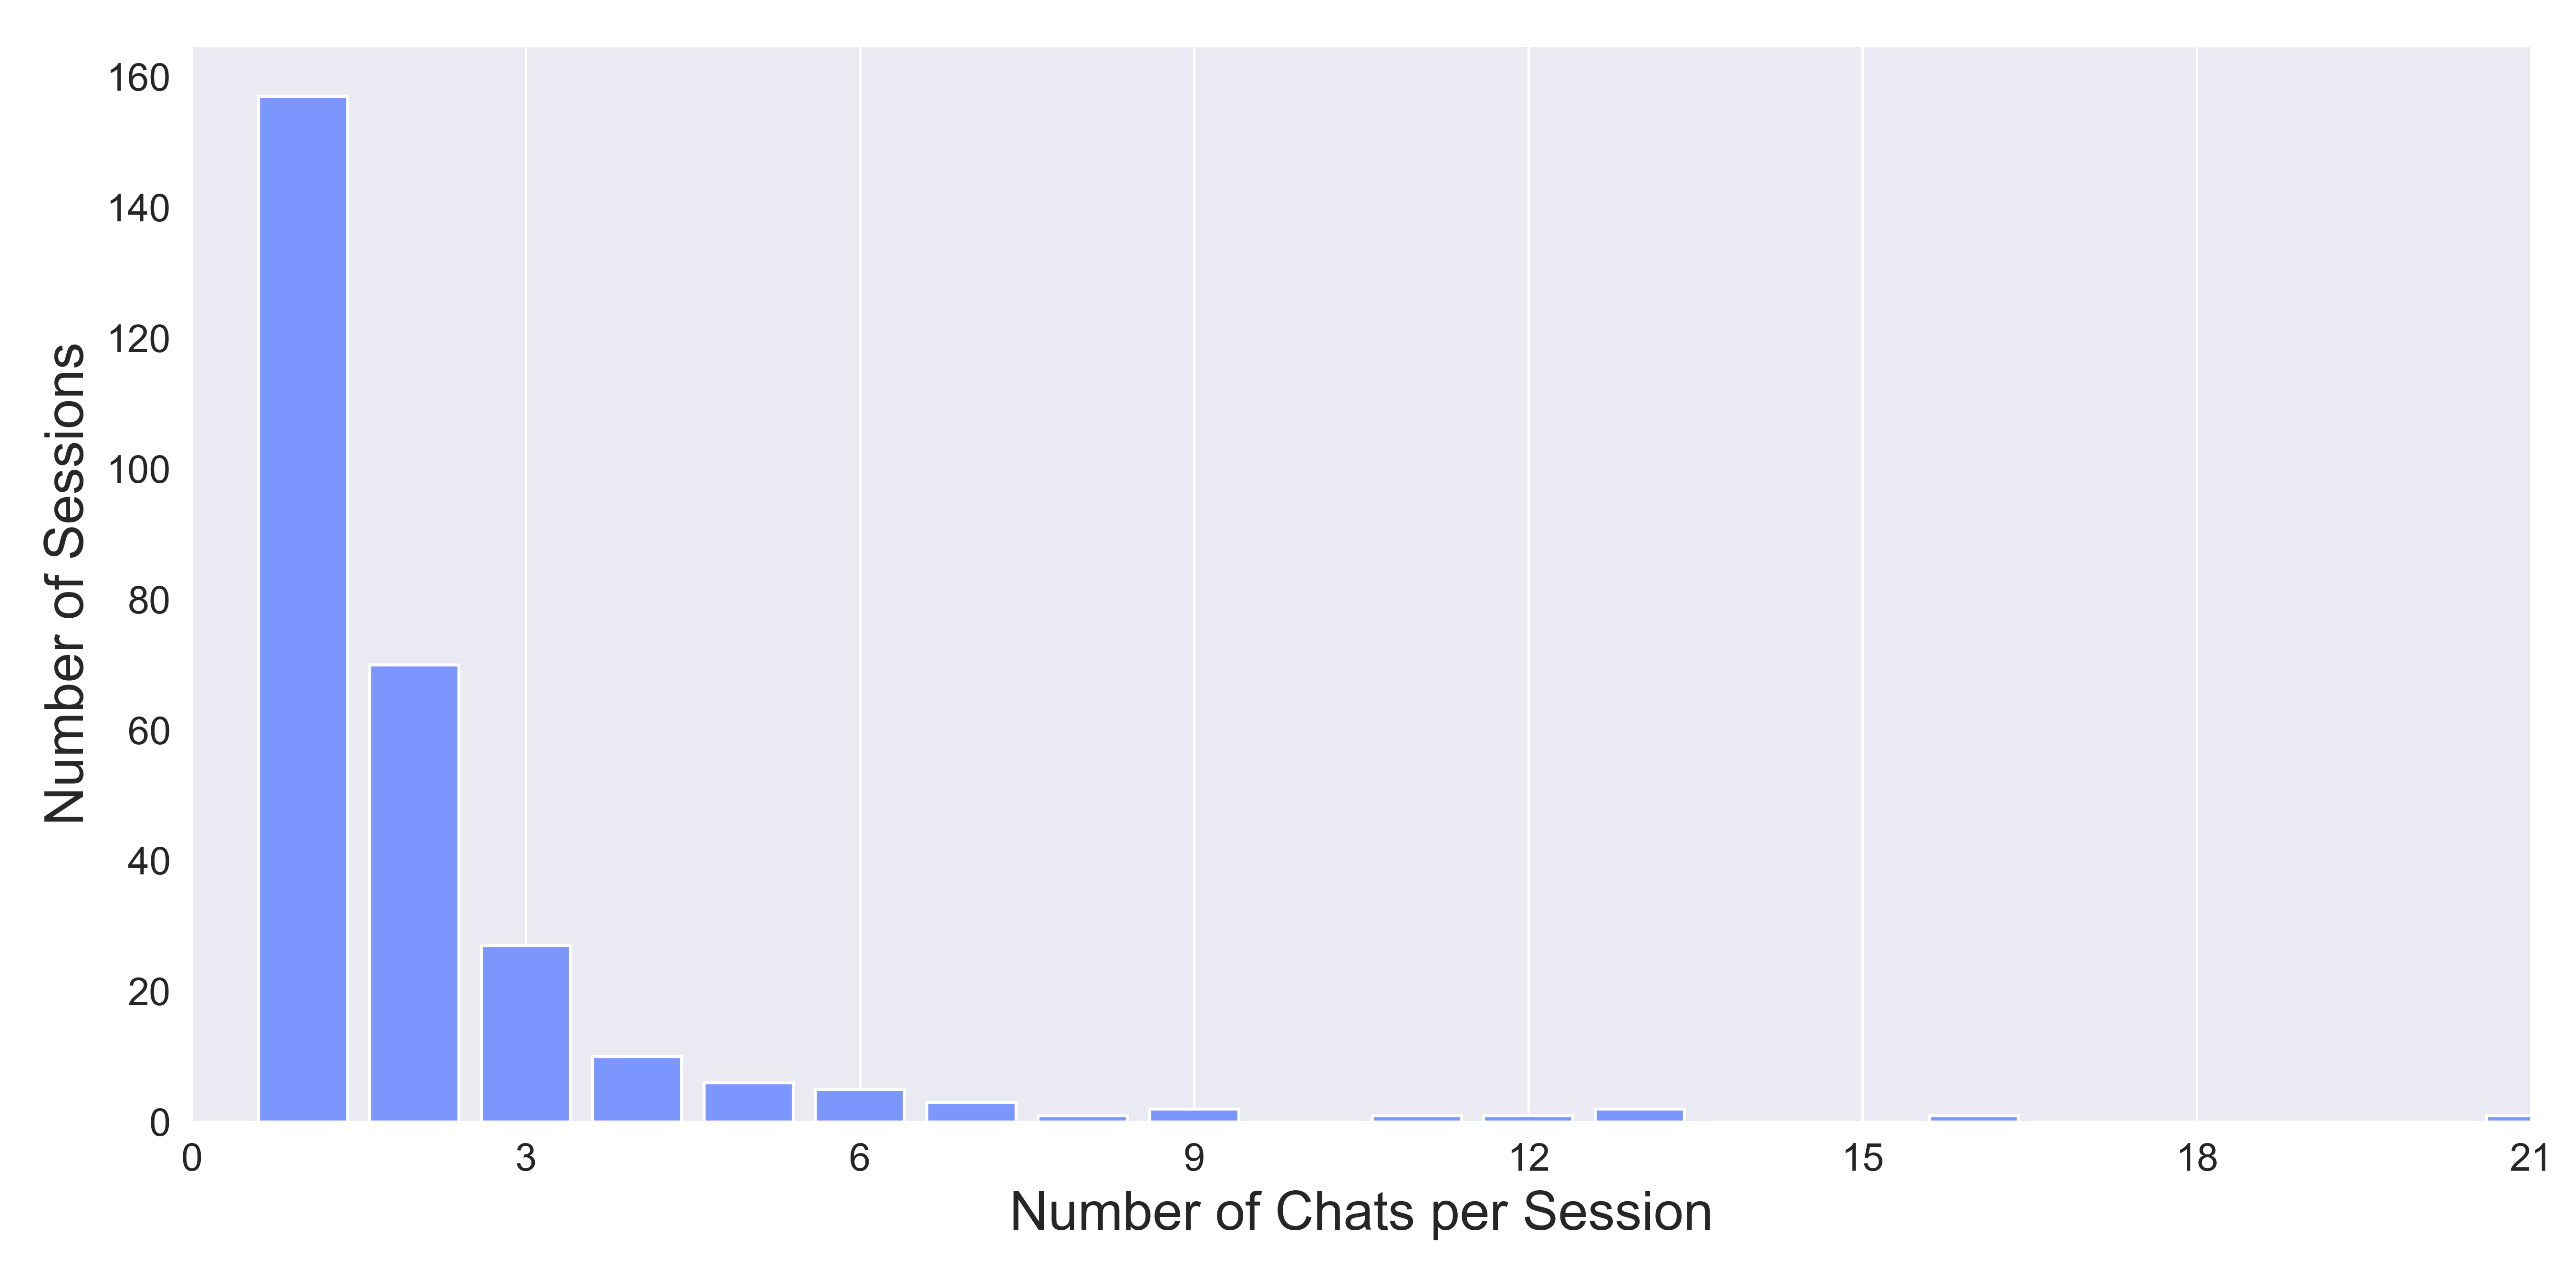
\includegraphics[width=\textwidth]{results/plots/assets/usage-12-number-of-sessions-with-number-of-chats.png}
    \caption{Number of sessions with each number of chats}
    \label{fig:usage_12_number_of_sessions_with_number_of_chats}
\end{figure}


\begin{figure}[H]
    \centering
    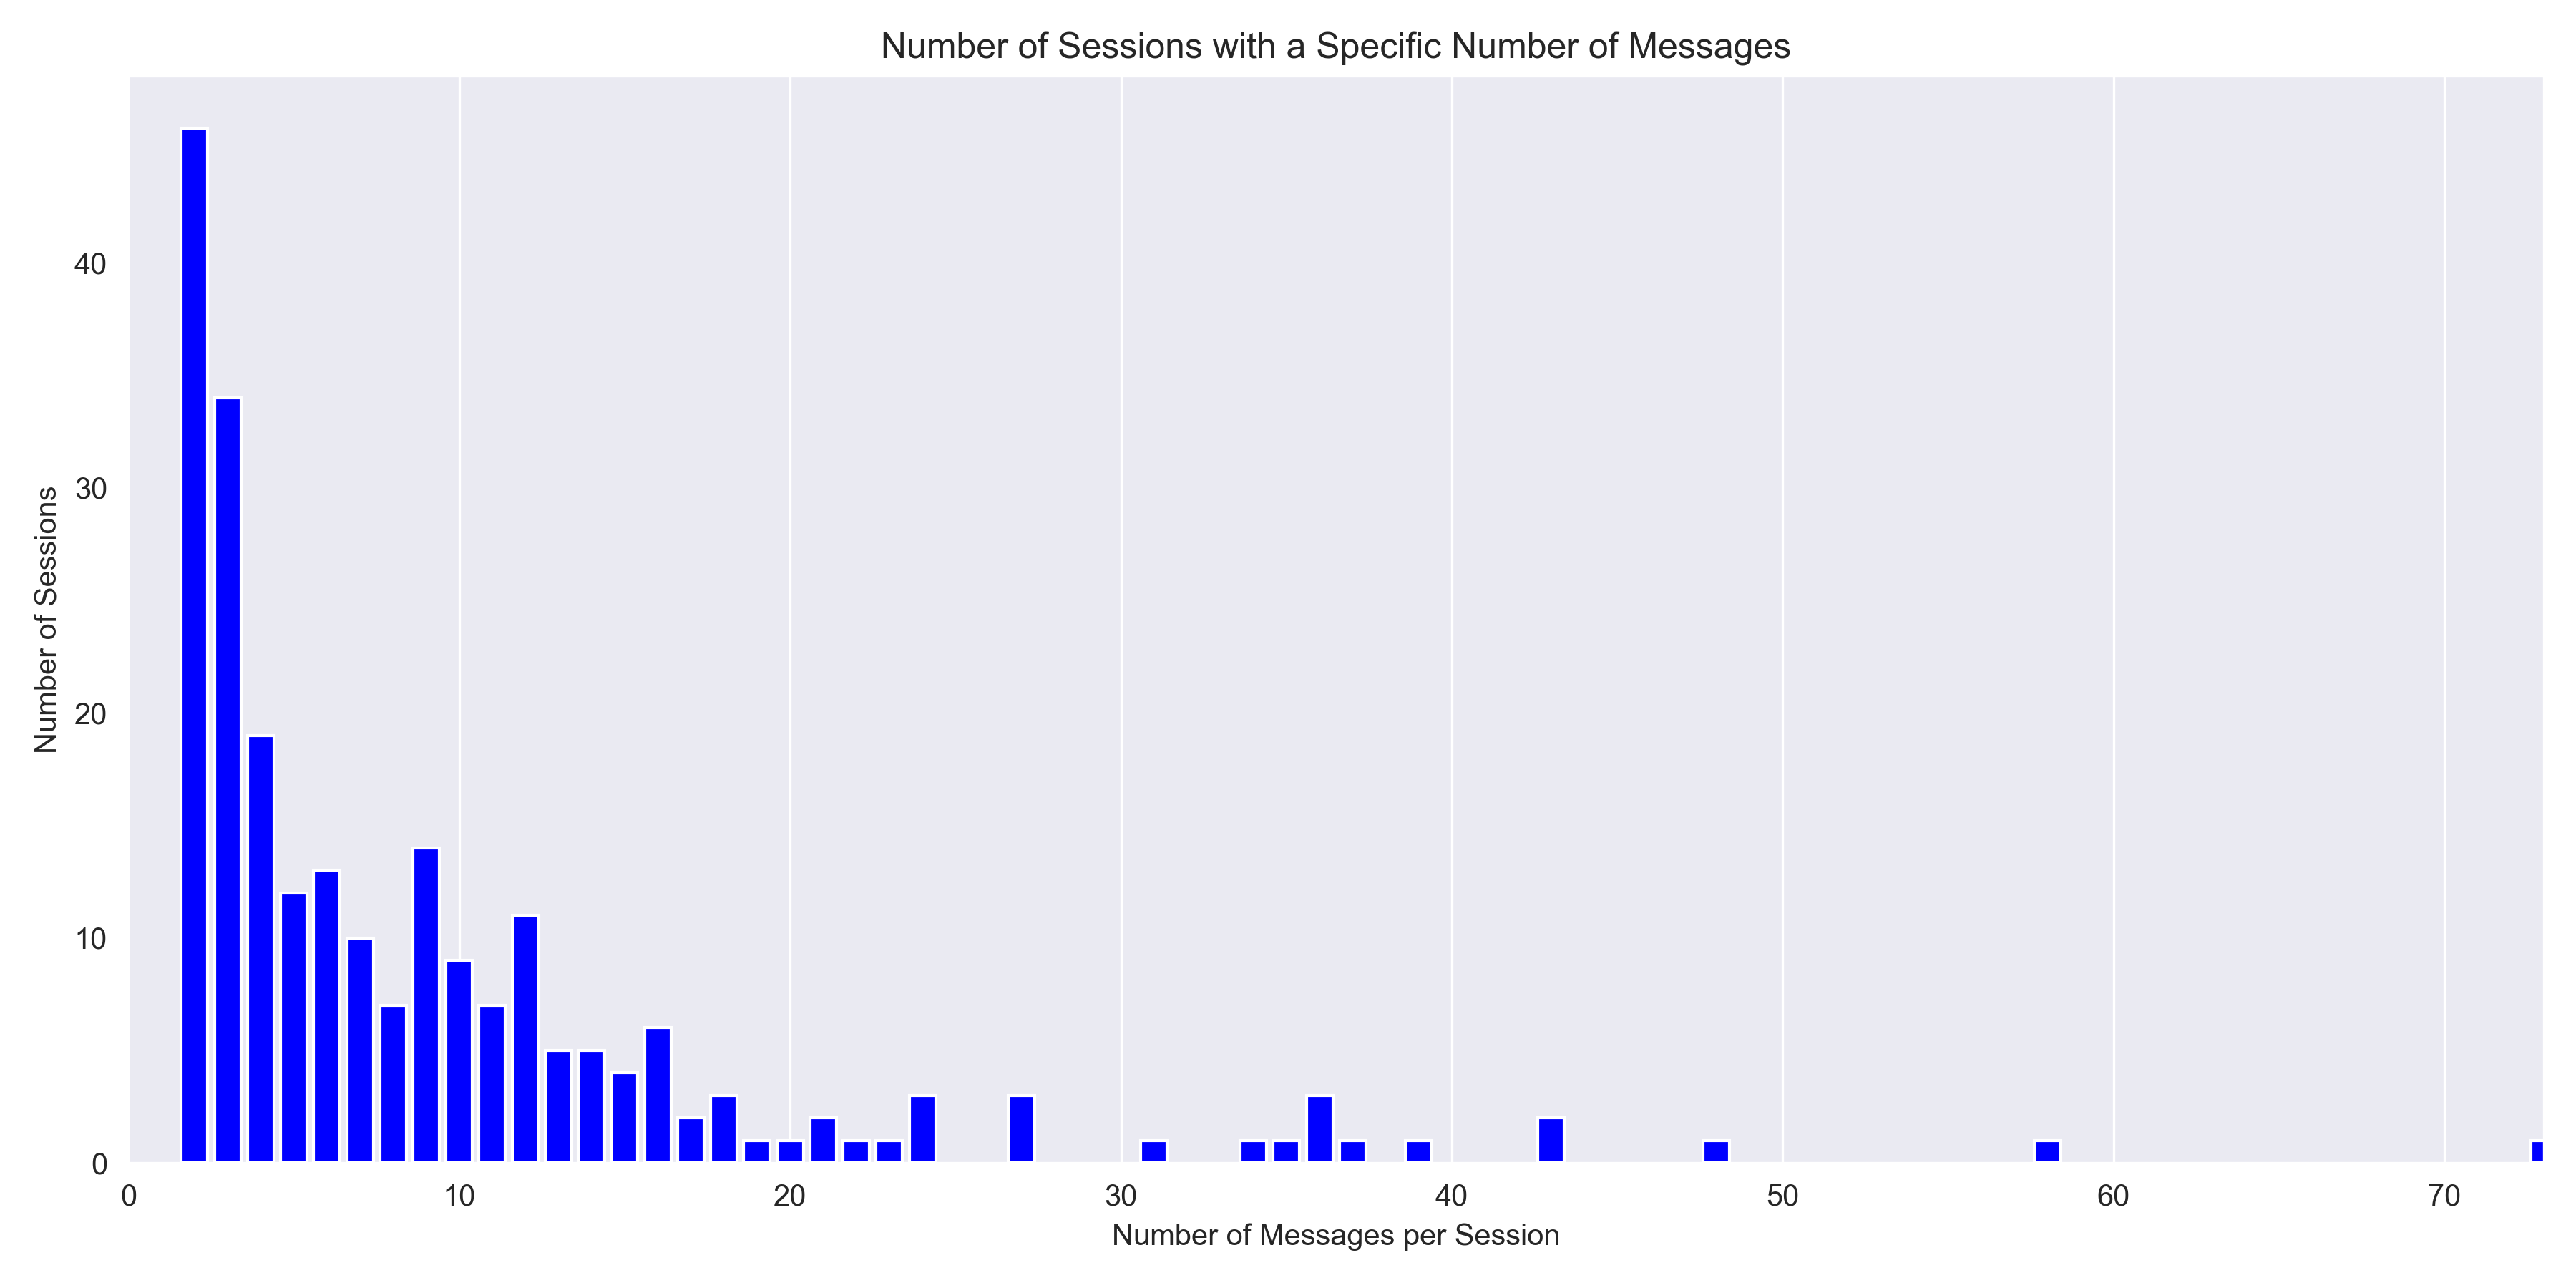
\includegraphics[width=\textwidth]{results/plots/assets/usage-13-number-of-sessions-with-number-of-messages.png}
    \caption{Number of sessions with each number of messages}
    \label{fig:usage_13_number_of_sessions_with_number_of_messages}
\end{figure}


\subsection{Open source v. Proprietary LLMs}


With regards to the feasibility of building AI assistants on open source technologies there are a number of metrics to look at for comparing open source \gls{LLM}s to proprietary language models. \autoref{tab:sessions_chats_and_messages_by_model} shows metrics for both models that were included in the experiment. The experiment was designed to sample between the included models randomly, and as we can see the number of sessions started between the two models are virtually the same. However, there are notable differences in the number of chats started and messages sent between the two. The proprietary model, \textit{GPT-4} by OpenAI, leads the open source model, \textit{Mistral-7B-Instruct-v0.2} by MistralAI. Section~\ref{sec:qualitative_analysis_of_user_responses} and \ref{sec:impact_of_llm_on_user_preferences} will showcase the user preferences with respect to these models, which could explain the discrepancy between two models with regards to simple usage metrics, which is what is shown in \autoref{tab:sessions_chats_and_messages_by_model}.



\begin{table}[H]
\centering
\scriptsize
\begin{tabular}{@{}lcccccc@{}}
\toprule
Model & No. Sessions & \% & No. Chats & \% & No. Messages & \% \\
\midrule
\textit{openai/gpt4} & \textbf{305} & \textbf{50.92} & \textbf{359} & \textbf{60.23} & \textbf{1141} & \textbf{52.29} \\
\textit{mistralai/Mistral-7B-Instruct-v0.2} & 294 & 49.08 & 237 & 39.77 & 1041 & 47.71 \\

\bottomrule
\end{tabular}
\caption{Statistics of Sessions, Chats, and Messages by Model}
\label{tab:sessions_chats_and_messages_by_model}
\end{table}



Looking at the operational performance of both models included in \autoref{tab:sessions_chats_and_messages_by_model}, there are two notable metrics that were measured in the experiment with respect to operating these models, more specifically metrics that doesn’t measure the quality of their responses (these are covered in \label{sec:impact_of_llm_on_user_preferences}). The metrics are; the response time for the model and time taken to generate queries. The latter is measuring what is generated by the system to query the index that was produced when crawling the course room. The \gls{LLM} is obviously used to generate the assistant's next message, but it is also used to generate a search query, based upon the current conversation between the assistant and the user. The time taken to generate this query is obviously important for the overall performance of the system.


\autoref{fig:performance_05_daily_average_response_time_including_pending_time} shows the daily average response for each model. This includes the time taken before a worker node had picked up the workload. This is important because in the event of high traffic to the system, \gls{LLM} tasks could be queued up and response times could increase. The chart shows that the two models are generally very similar in terms of the time it takes them to produce a reply to the user's question. It is notable however, that the open source alternative (\textit{Mistral-7B-Instruct-v0.2}) has higher peaks on certain days.


\begin{figure}[H]
    \centering
    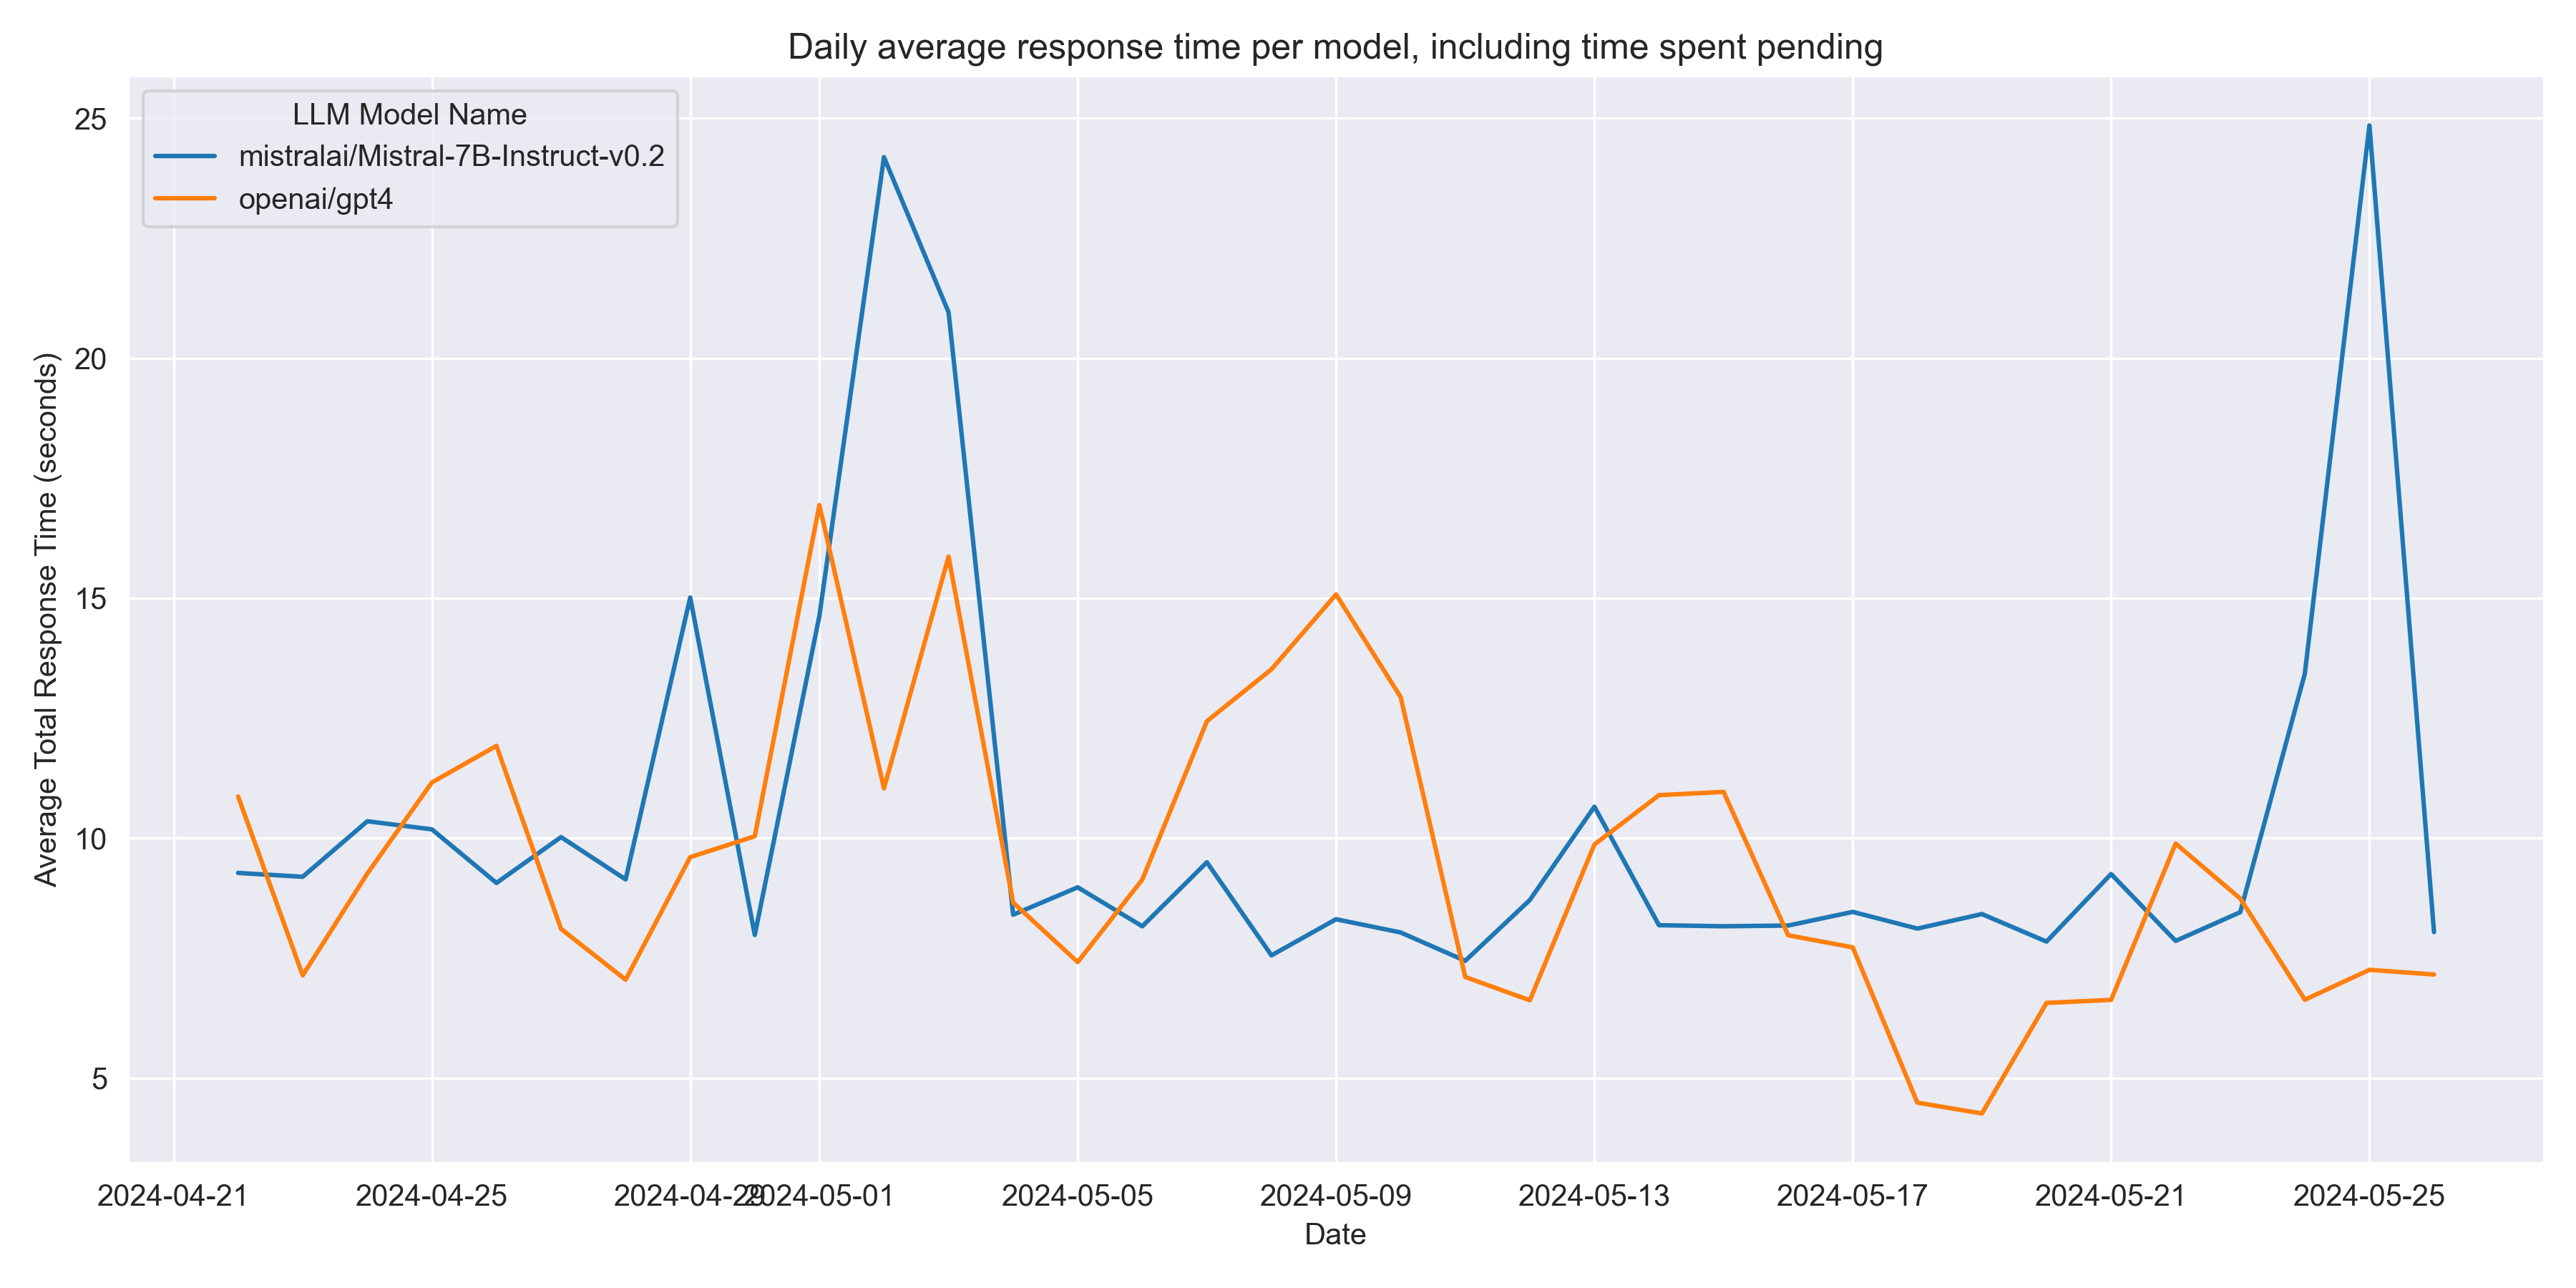
\includegraphics[width=\textwidth]{results/plots/assets/performance-05-daily-average-response-time-per-model-including-pending-time.png}
    \caption{How long each model took to generate a response, including time spent pending.}
    \label{fig:performance_04_daily_average_response_time_including_pending_time}
\end{figure}


\autoref{fig:performance_06_generating_queries} shows the time taken to produce queries. Similar to what could be said about \autoref{fig:performance_05_daily_average_response_time_including_pending_time}, both models perform very similarly. However, in this metric the open source alternative is faster. The reason the open source model outperforms \textit{GPT-4} on this metric is likely due to the higher latency sometimes observed on the OpenAI API. The custom built solution to operate \gls{LLM} for this study exhibits much lower latency.


\begin{figure}[H]
    \centering
    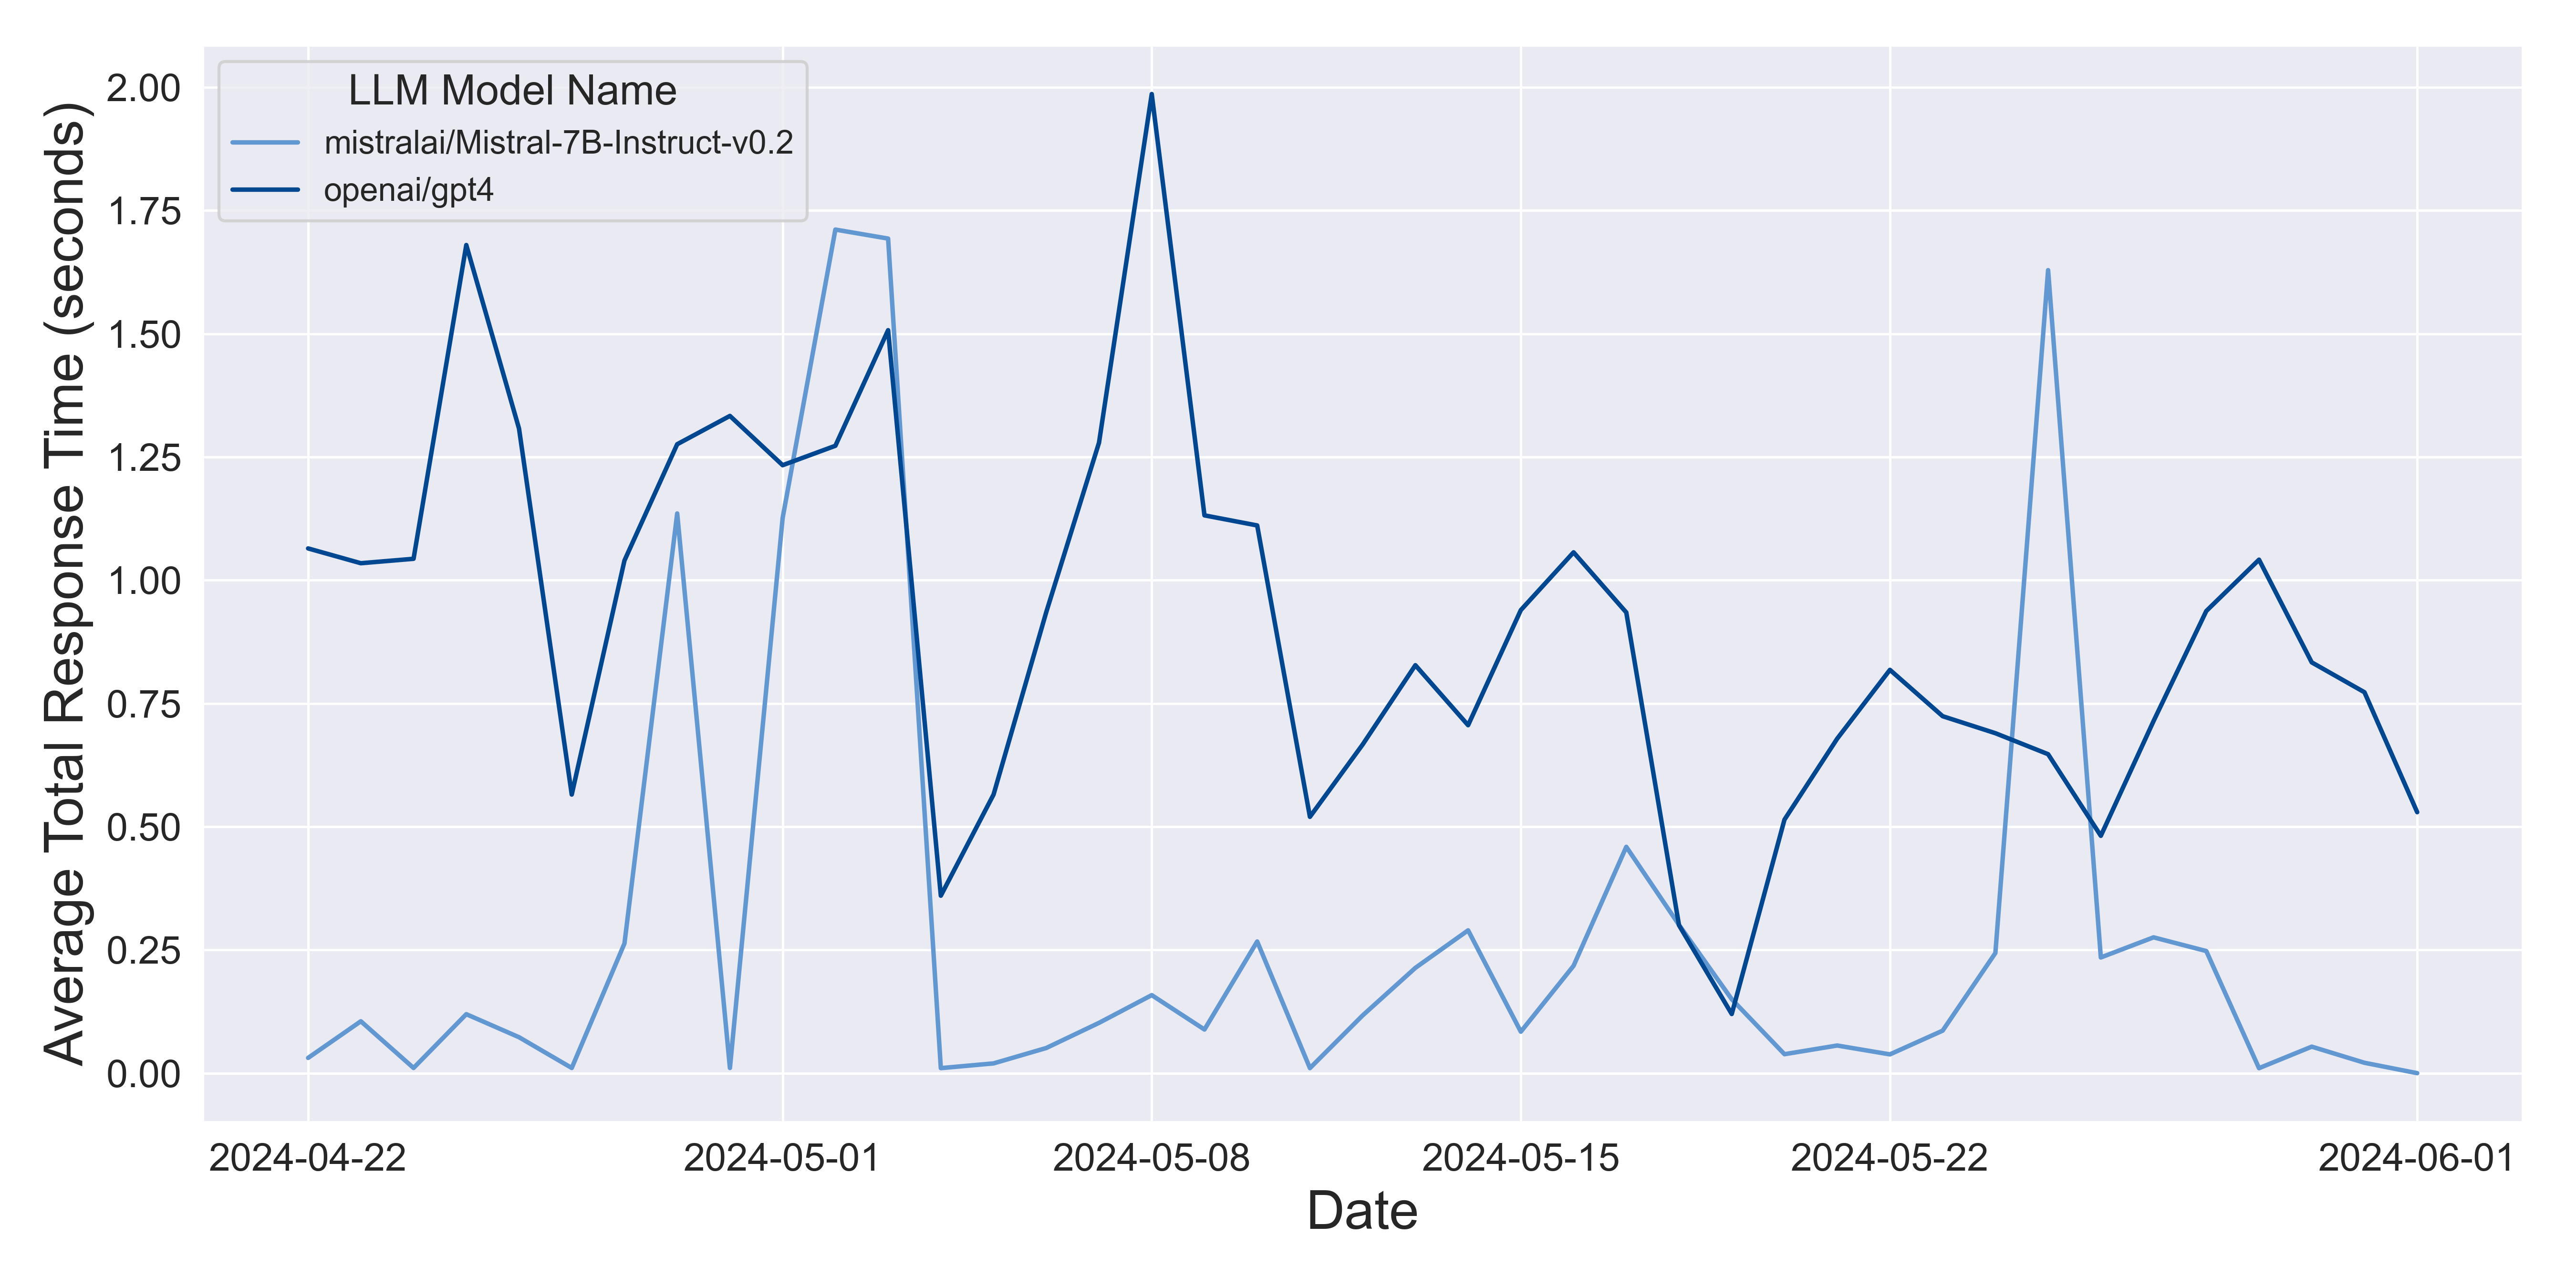
\includegraphics[width=1\textwidth]{results/plots/assets/performance-06-generating-queries.png}
    \caption{How long each model took to generate queries.}
    \label{fig:performance_06_generating_queries}
\end{figure}


\subsection{Open source v. Proprietary Embedding functions}


The intention of the research in this thesis was to compare open source embedding functions with proprietary alternatives commonly used in \gls{RAG}-based applications. In addition to this, the experiment was also designed to be able to measure vector search as a retrieval technique, with traditional full text search. However, due to the number of students that participated in the study, no configuration was used that didn’t use the vector search strategy with the embedding function \textit{text-embedding-3-large} by OpenAI \cite{openai_new_2024}. So no metrics were captured in the retrieval phase for any other strategy or model. The retrieval time taken for the model that was used is shown in \autoref{fig:performance_07_embedding_function_query_performance}. Metrics were, however, captured during the indexing phase on other models.


\begin{figure}[H]
    \centering
    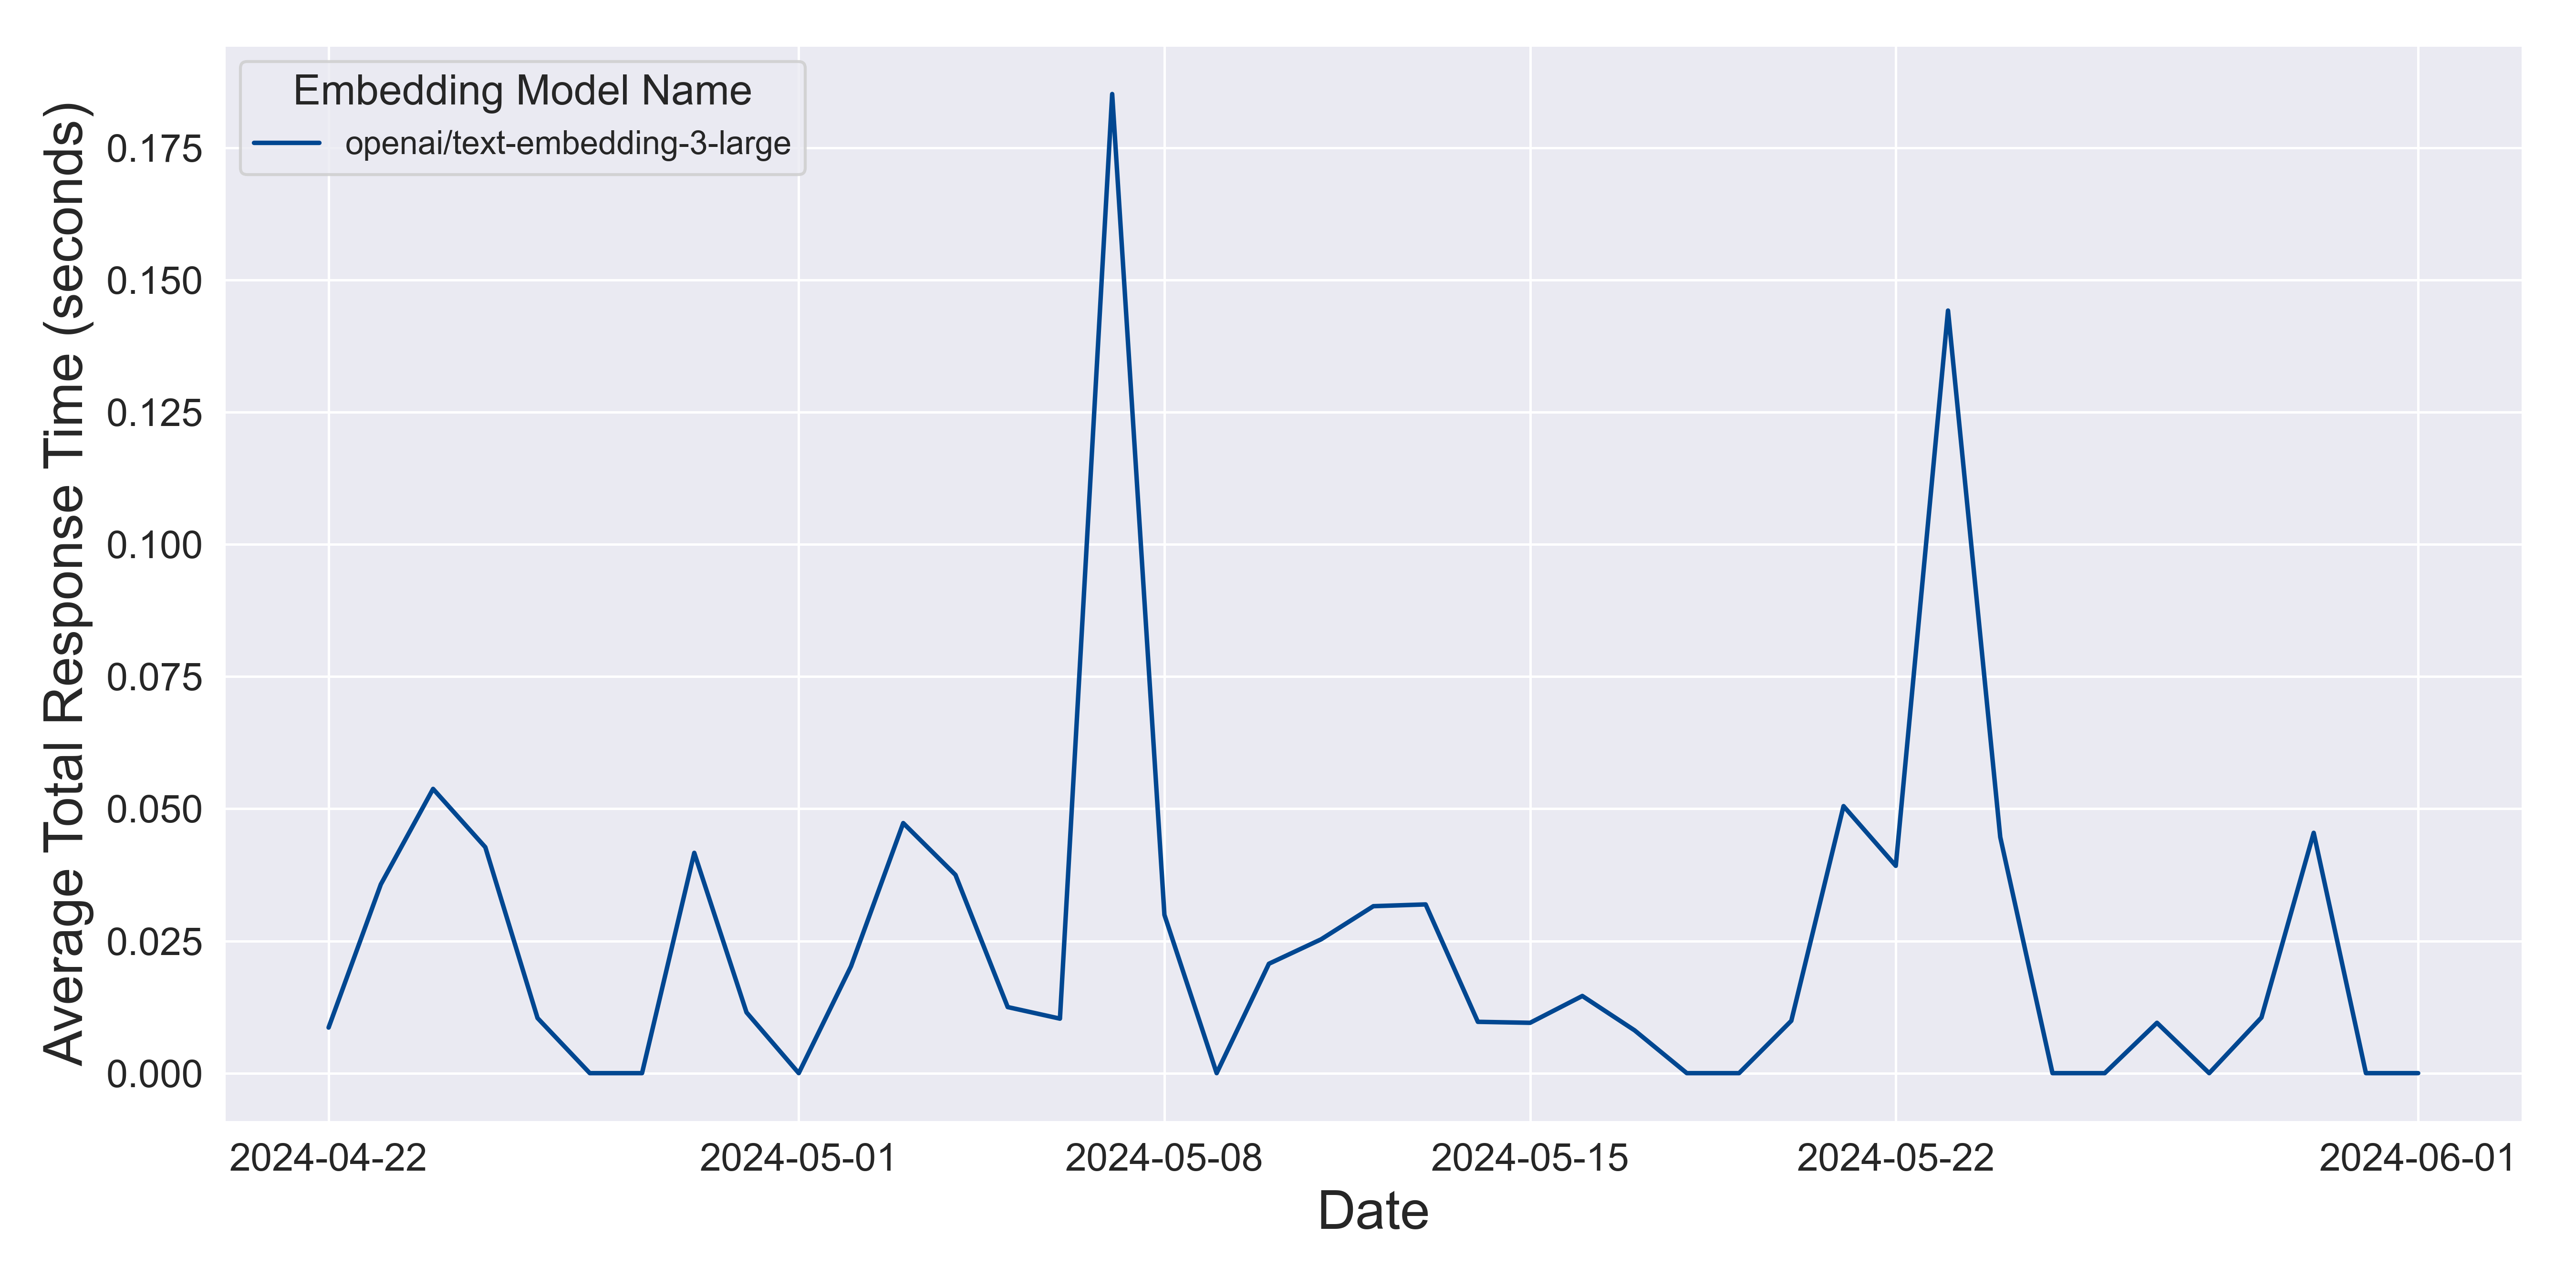
\includegraphics[width=1\textwidth]{results/plots/assets/performance-07-embedding-function-query-performance.png}
    \caption{How long each model took to execute queries.}
    \label{fig:performance_07_embedding_function_query_performance}
\end{figure}


\subsubsection{Understanding the indexing}
\label{sec:understanding_indexing}


The indexing of course rooms was done regularly. It wasn’t done on a schedule, it was instead done on an ad-hoc basis whenever a course was updated with new content. \autoref{fig:performance_01_timeline_of_snapshots_taken} shows a timeline for each course which includes the date for when each snapshot of the course room was taken.


\begin{figure}[H]
    \centering
    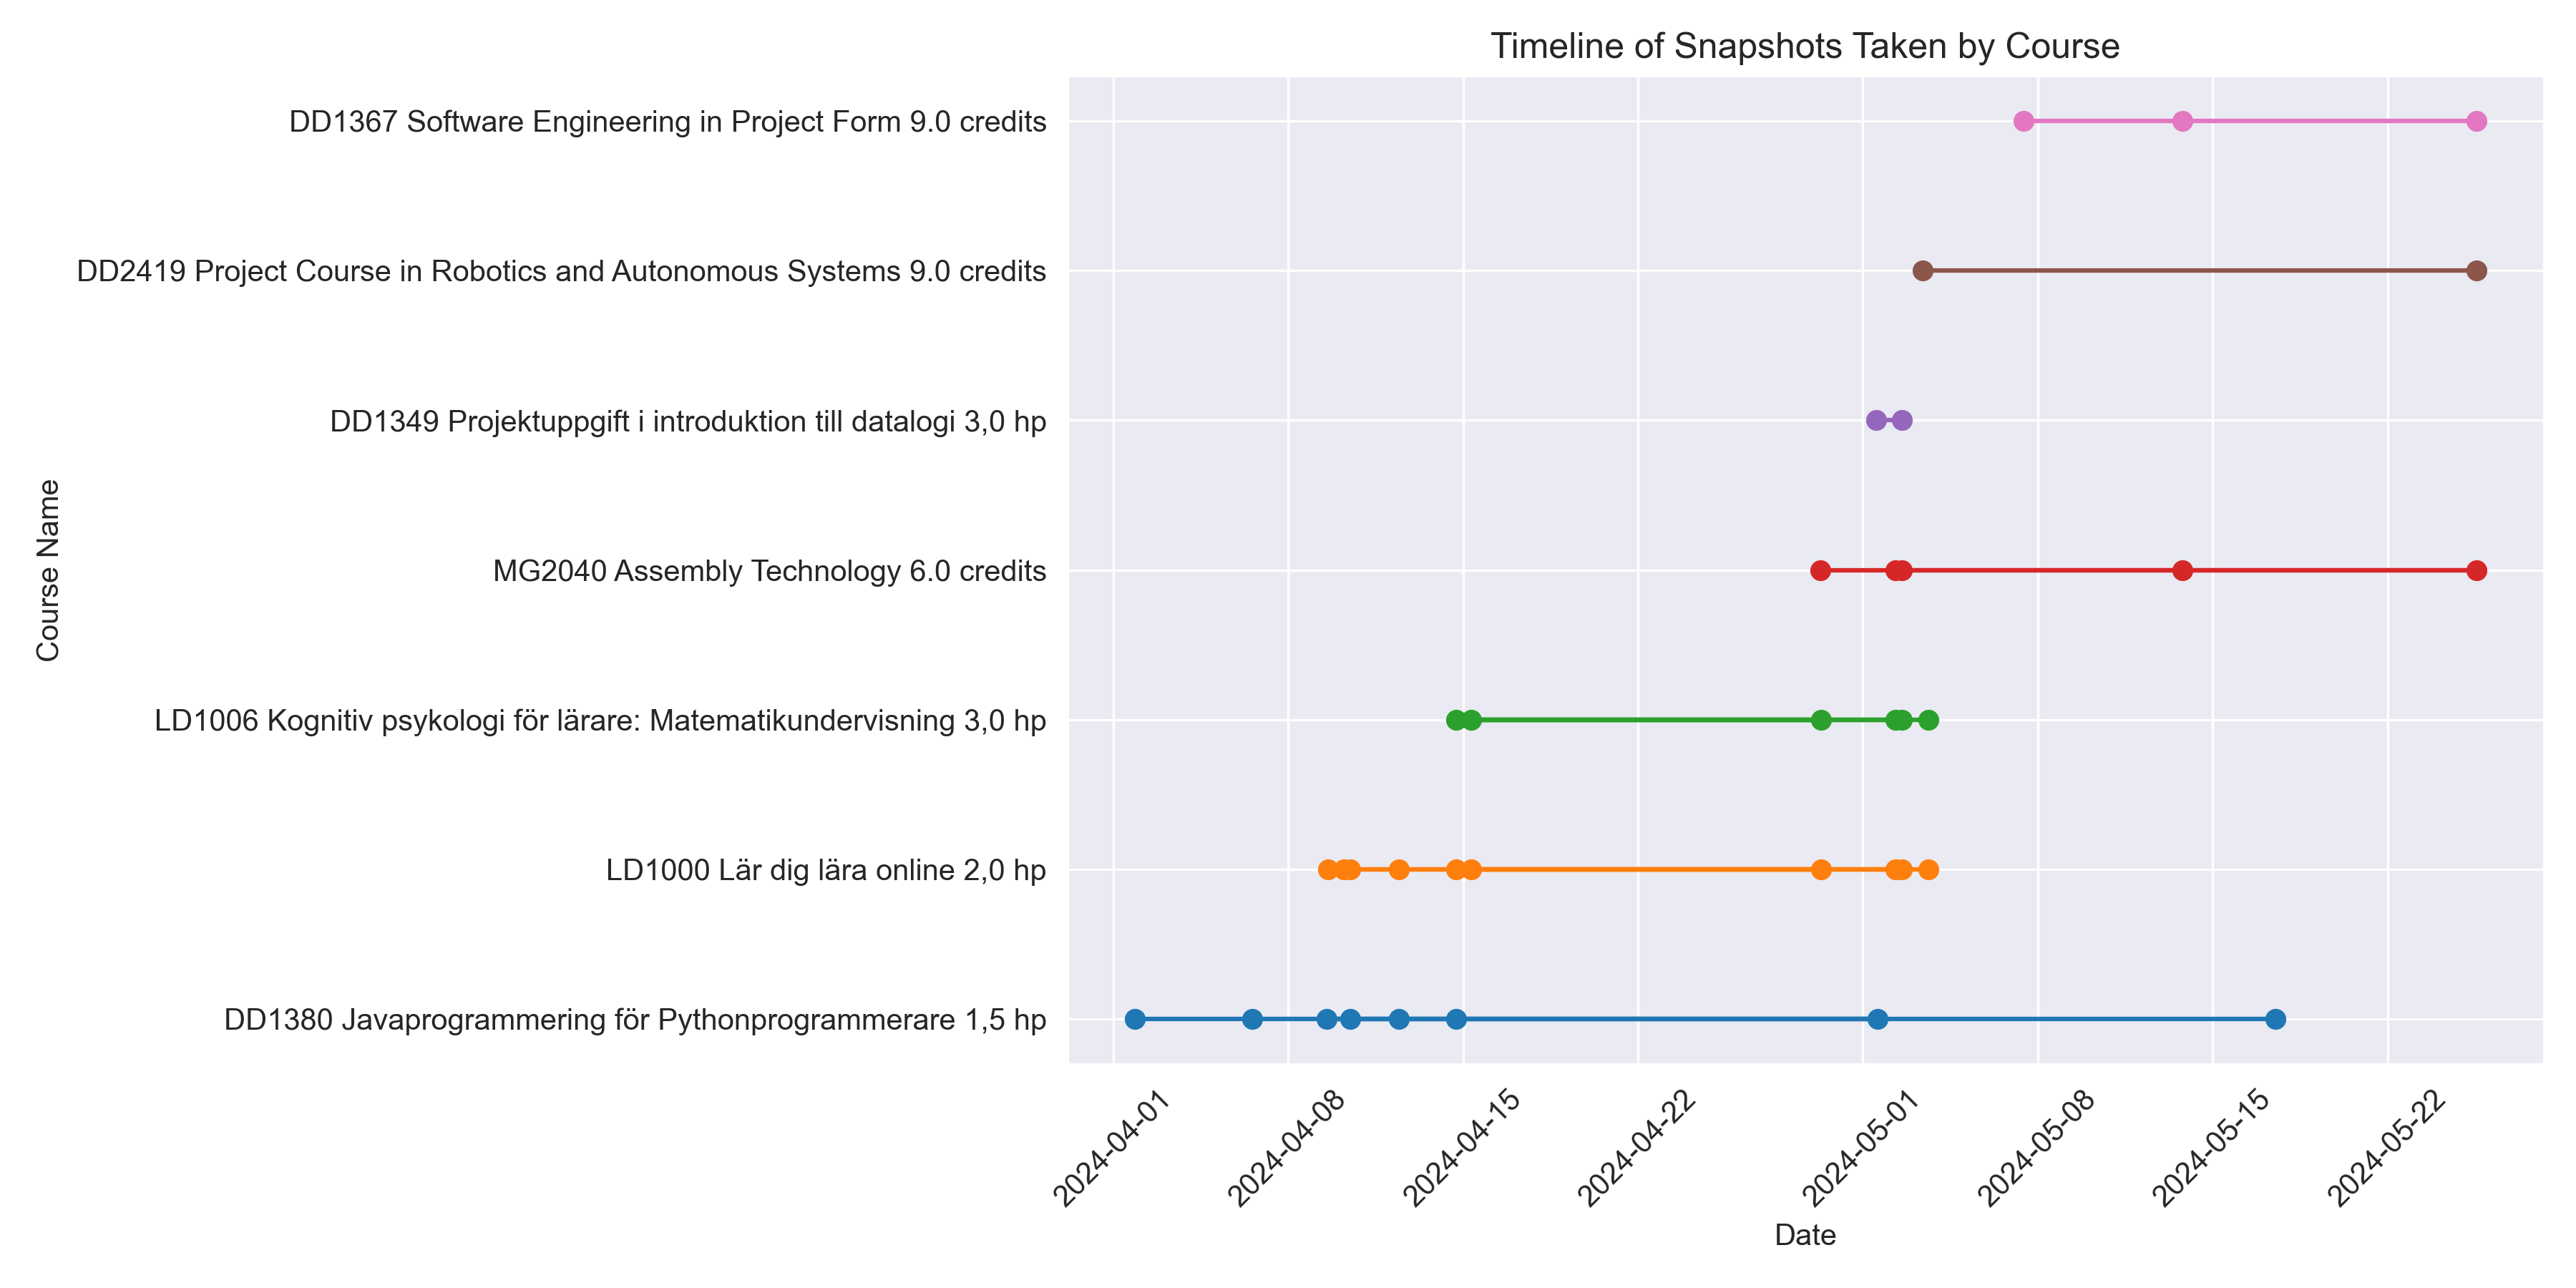
\includegraphics[width=\textwidth]{results/plots/assets/performance-01-timeline-of-snapshots-taken.png}
    \caption{Timeline for each snapshot taken of the courses participating in the study.}
    \label{fig:performance_01_timeline_of_snapshots_taken}
\end{figure}


Each course room is different and includes pages and content of varying length. No exact metric for how much content was included in each course room is presented in this section, however \autoref{fig:performance_02_urls_per_course} shows how many urls the crawler found in each course, and how many of them were indexed. This is an imperfect, yet decent proxy for how "large" a course room was.


\begin{figure}[H]
    \centering
    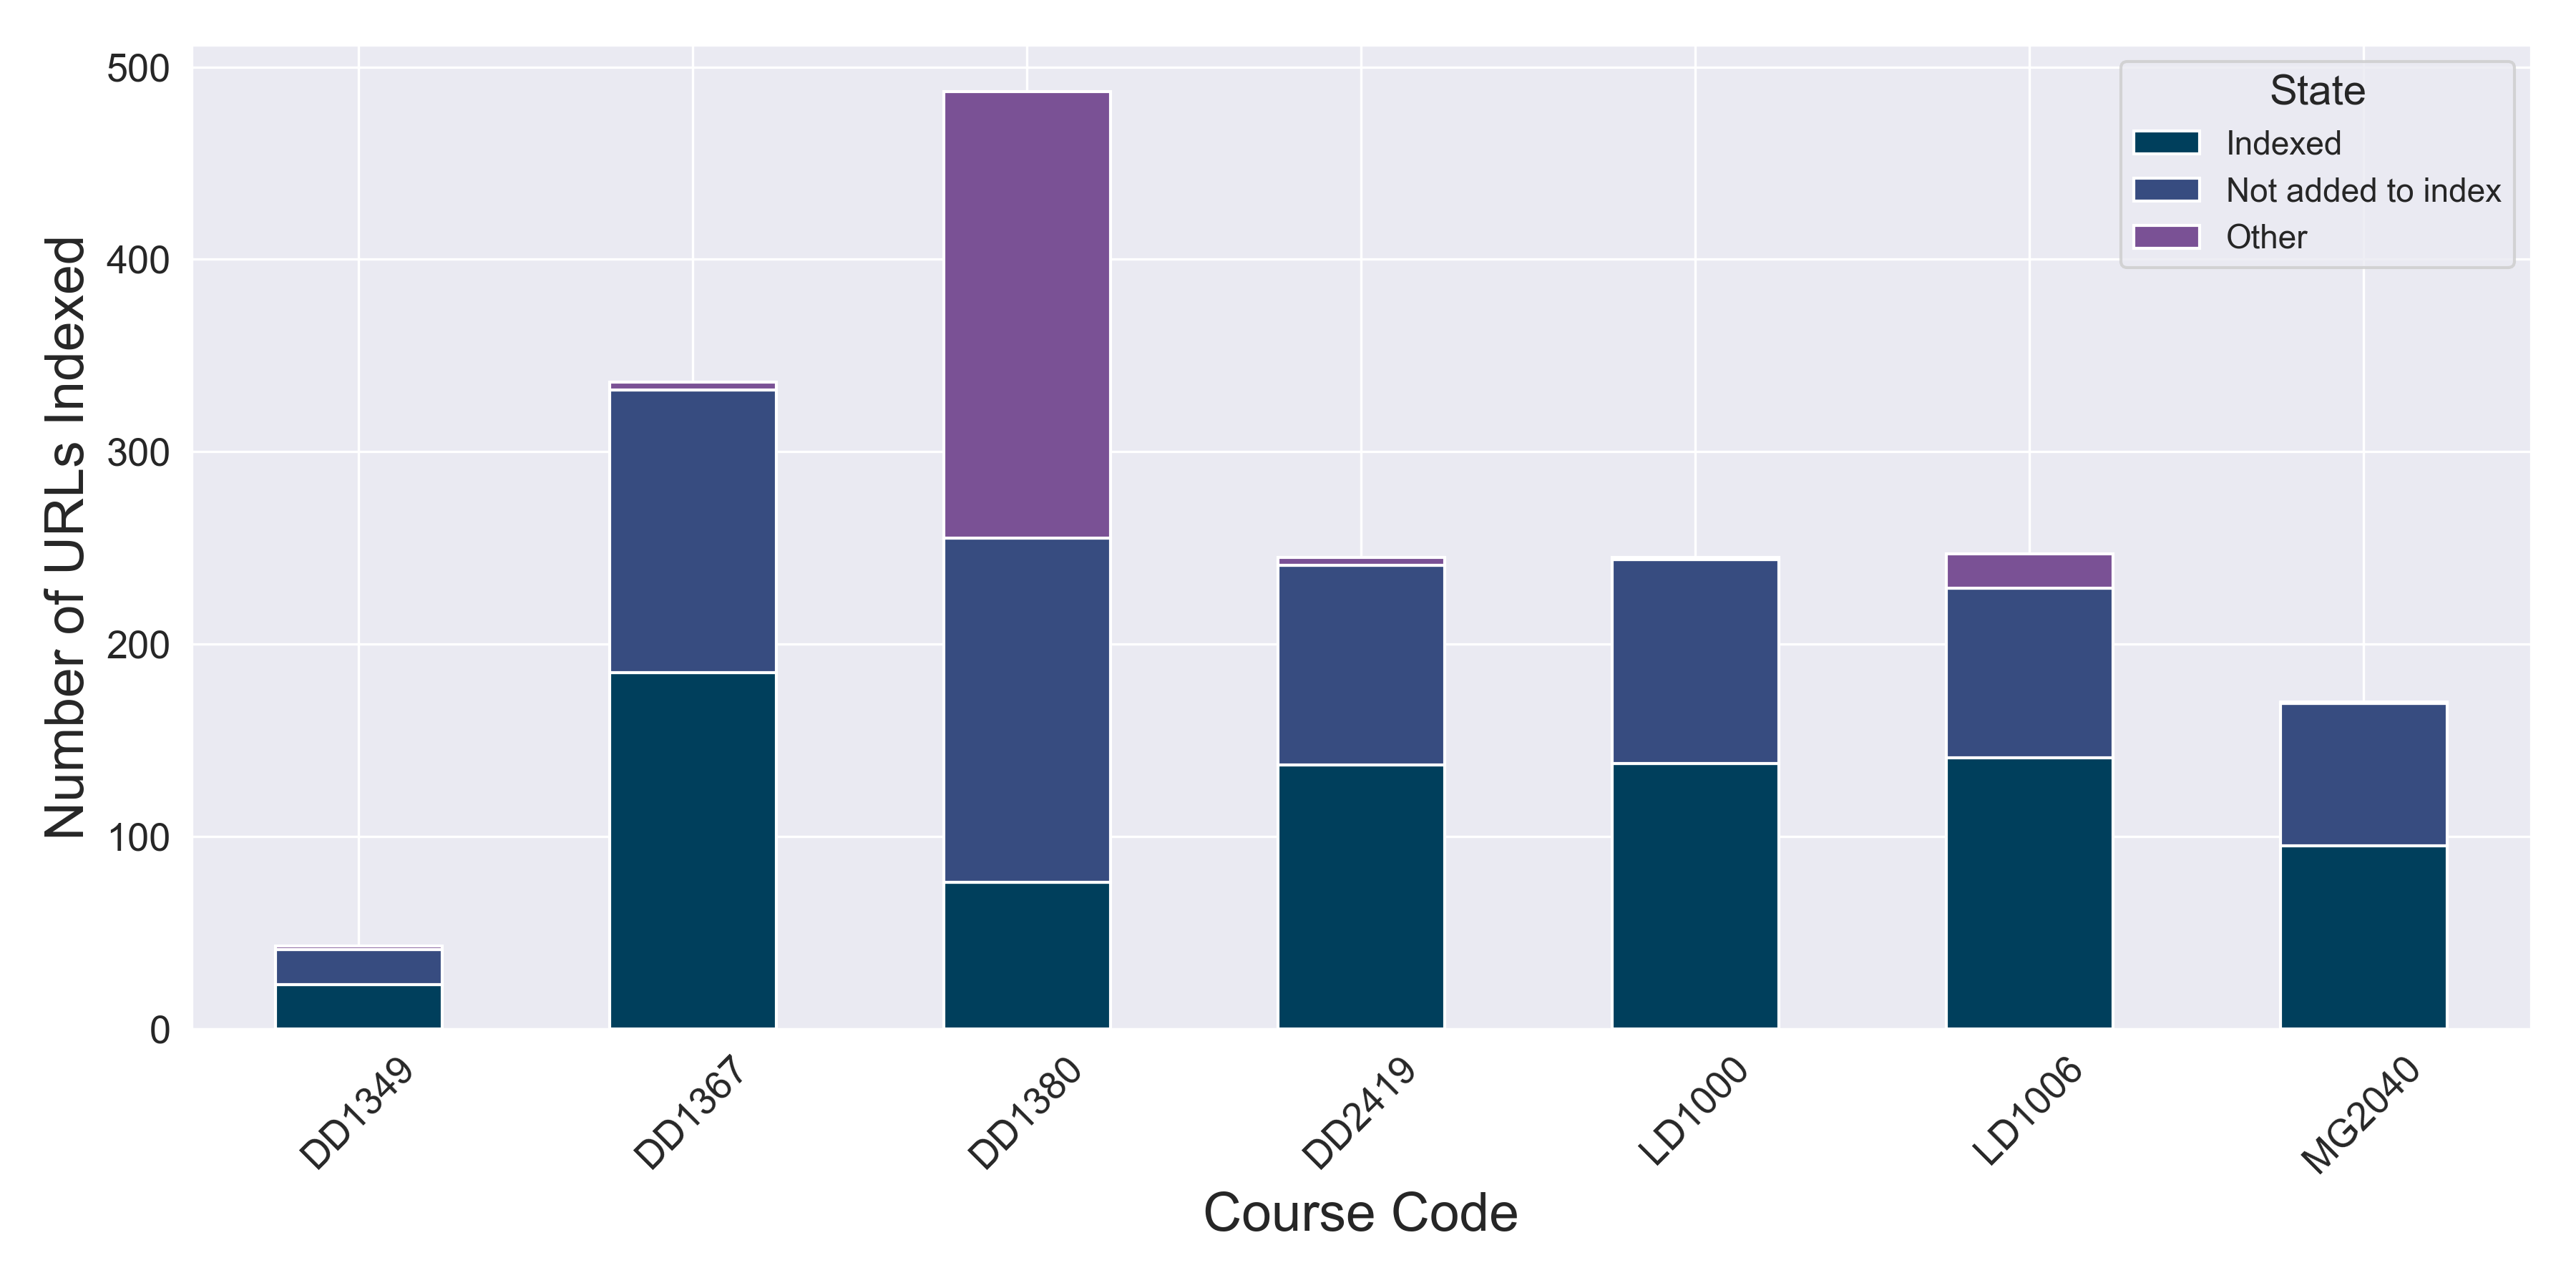
\includegraphics[width=1\textwidth]{results/plots/assets/performance-02-urls-per-course.png}
    \caption{Number of URLs included in the most recent snapshot of each course.}
    \label{fig:performance_02_urls_per_course}
\end{figure}


To understand why the size of the course room is relevant we need to look at \autoref{fig:performance_03_index_time}, that shows how long each course room took to index. We can see that indexing time for the same course room vary a lot. The reason for this is not that the size of the course room varies over time. Looking at \autoref{fig:performance_03_index_time} we can see that the higher values occur when snapshots are taken simultaneously. The way indexing time is measured is by taking the time between the first url in a course room being crawled, and the last time a url was indexed in that snapshot. \autoref{fig:performance_03_index_time} suggests that there is an operation that takes a lot of time, and the indexer gets overloaded when a lot of courses are being indexed at the same time. Section~\ref{sec:measuring_indexing_performance} will show that this is due to the performance of the open source embedding function used in the experiments.


\begin{figure}[H]
    \centering
    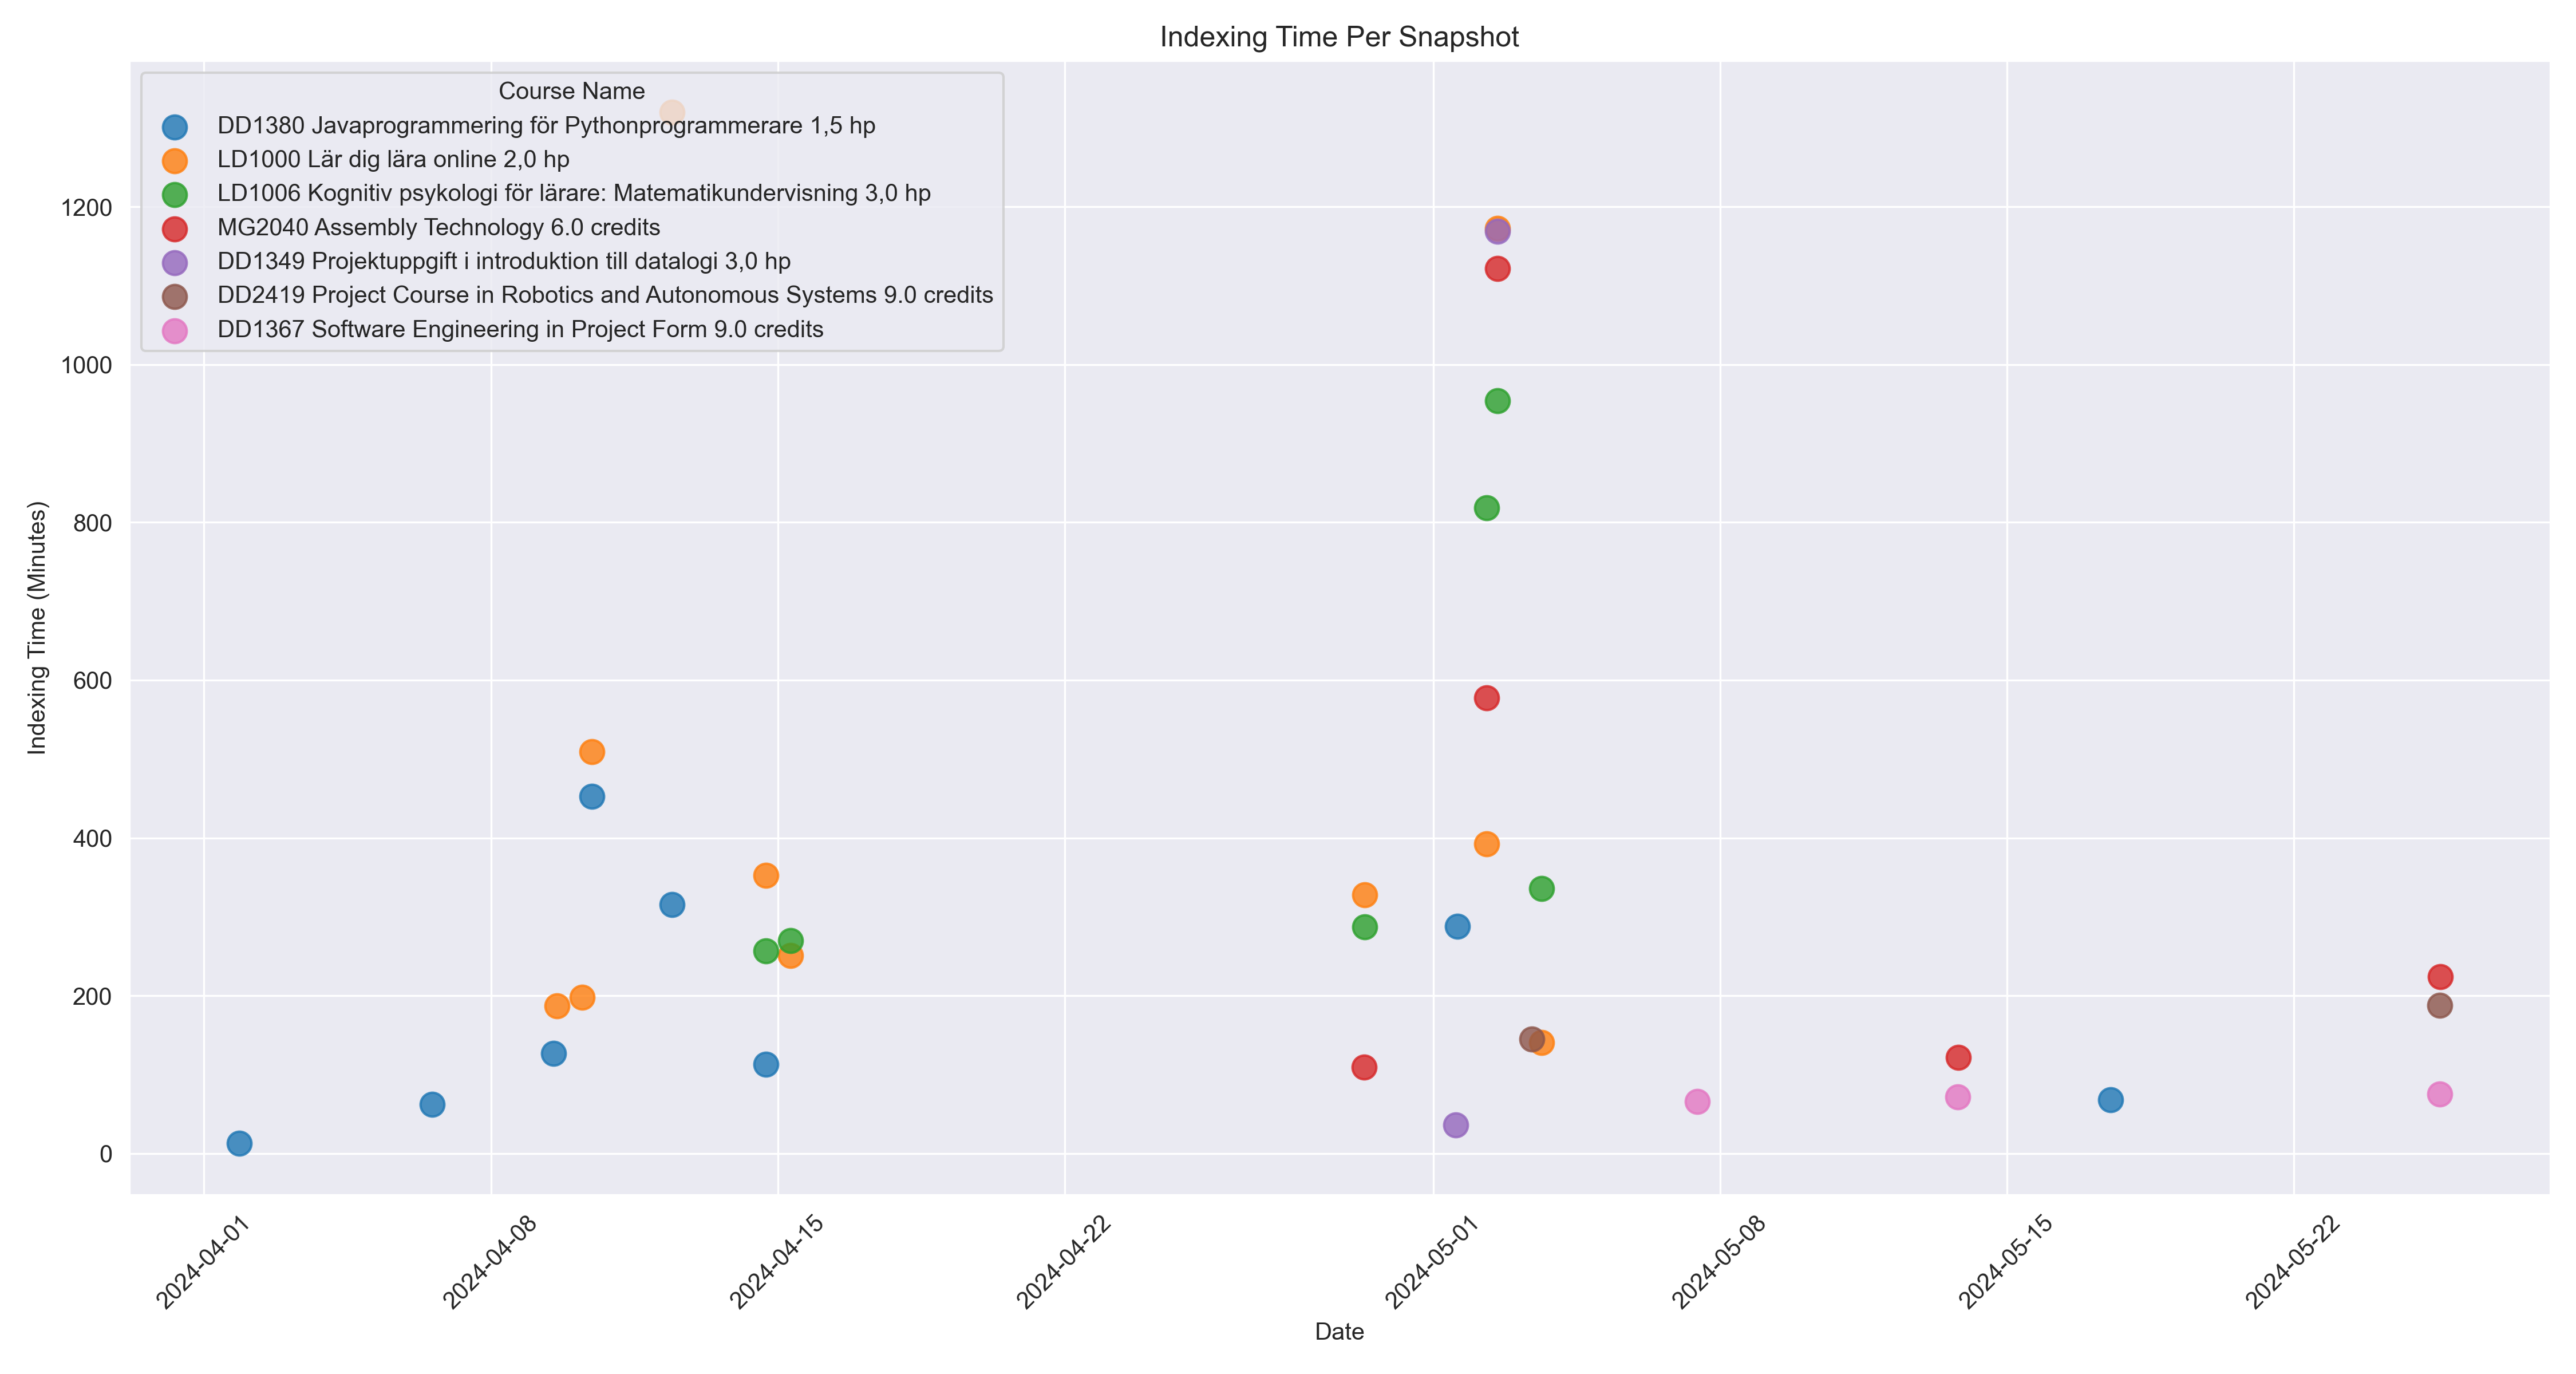
\includegraphics[width=1\textwidth]{results/plots/assets/performance-03-index-time.png}
    \caption{How long indexing took per snapshot.}
    \label{fig:performance_03_index_time}
\end{figure}


\subsubsection{Measuring indexing performance}
\label{sec:measuring_indexing_performance}


As shown and explained in section~\ref{sec:understanding_indexing} the most time consuming part of indexing a course room was computing the embeddings for all documents added to the index. \autoref{tab:average_response_time_embedding_functions} shows the open source embedding function used in the experiment, Salesforces’ \textit{SFR-Embedding-Mistral}\cite{meng_sfr-embedding-mistral_2024}, which was chosen because it had the highest score on the \gls{MTEB}-benchmark \footnote{As of \today}, is two orders of magnitude slower than \textit{text-embedding-3-large}, the currently best embedding function developed by OpenAI. The reason for this was likely the execution environment chosen for the open source candidate.



\begin{table}[H]
\centering
\begin{tabular}{@{}lc@{}}
\toprule
Model Name & Average Response Time (seconds) \\
\midrule
\textit{Salesforce/SFR-Embedding-Mistral} & 103.51s \\
\textit{openai/text-embedding-3-large} & \textbf{0.03}s \\

\bottomrule
\end{tabular}
\caption{Average Total Response Time per Embedding Function}
\label{tab:average_response_time_embedding_functions}
\end{table}



During the experiment the embedding functions utilised the same servers that ran the open source \gls{LLM}s. To utilise the hardware rented for this thesis optimally, the open source embedding models were executed on the unutilised CPUs of the servers which ran the \gls{LLM}s on their attached GPU devices. The embedding models are, as opposed to the \gls{LLM}s at least feasible to run using a CPU only. However, as shown in \autoref{tab:average_response_time_embedding_functions}, this had quite a drastic impact on the indexing performance.


Had the open source models been used for retrieval, the performance difference would likely not have been as big. As shown in \autoref{tab:tab:average_response_time_by_length_embedding_functions} the difference in computation time between \textit{GPT-4} and \textit{SFR-Embedding-Mistra} is much smaller for smaller documents. Computing the embedding of a user query, which is what is done during retrieval, equates to computing the embedding for a very small document.



\begin{table}[H]
\centering
\scriptsize
\begin{tabular}{@{}lcccccc@{}}
\toprule
Prompt Length & 0-256 & 257-512 & 513-1024 & 1025-2048 & 2049-4096 & 4097-8192 \\
\midrule
Model Name &  &  &  &  &  &  \\
\textit{Salesforce/SFR-Embedding-Mistral} & 14.24s & 17.51s & 25.9s & 48.6s & 102.56s & 153.31s \\
\textit{openai/text-embedding-3-large} & \textbf{0.0}s & \textbf{0.02}s & \textbf{0.02}s & \textbf{0.06}s & \textbf{0.02}s & \textbf{0.03}s \\

\bottomrule
\end{tabular}
\caption{Average Total Response Time per Embedding Function and Prompt Length}
\label{tab:response_time_by_length}
\end{table}





\section{The impact of different LLM models on the speed, accuracy and reliability of responses}
\label{sec:impact_of_llm_on_user_preferences}


This section will present and analyse the gathered data on user preference and technological efficacy of different tools and technologies such as different \gls{RAG} toolchains and \gls{LLM}, as outlined in section~\ref{sec:goals}.


\subsection{Thumbs up/Thumbs down responses to FAQ questions}


After each response to a question that was selected from the frequently asked questions (FAQs) that were shown before a user had sent any messages, as shown in \autoref{fig:faq_questions}, the user was presented with an optional binary thumbs up/down vote on the quality of the response. Both had a tooltip that said \textit{"This was a good response"} and \textit{"This was a bad response"} respectively. \autoref{fig:feedback_01_frequency_of_answer_for_question_2e09fd} shows how the participants in the study voted. Generally, it can be observed that users had a positive response to the replies produced to the FAQs. Almost twice as many positive answers were recorded as negative responses.


Looking at the breakdown per model, the open-source alternative \textit{Mistral-7B-Instruct-v0.2}, had almost the same amount of positive and negative responses, which can be seen in \autoref{fig:feedback_02_frequency_of_answer_for_question_per_model_2e09fd}. The proprietary model \textit{GPT-4} had a significantly higher proportion of positive responses, which indicates a generally more favourable reception from the participants in the study.


\begin{figure}[H]
    \centering
    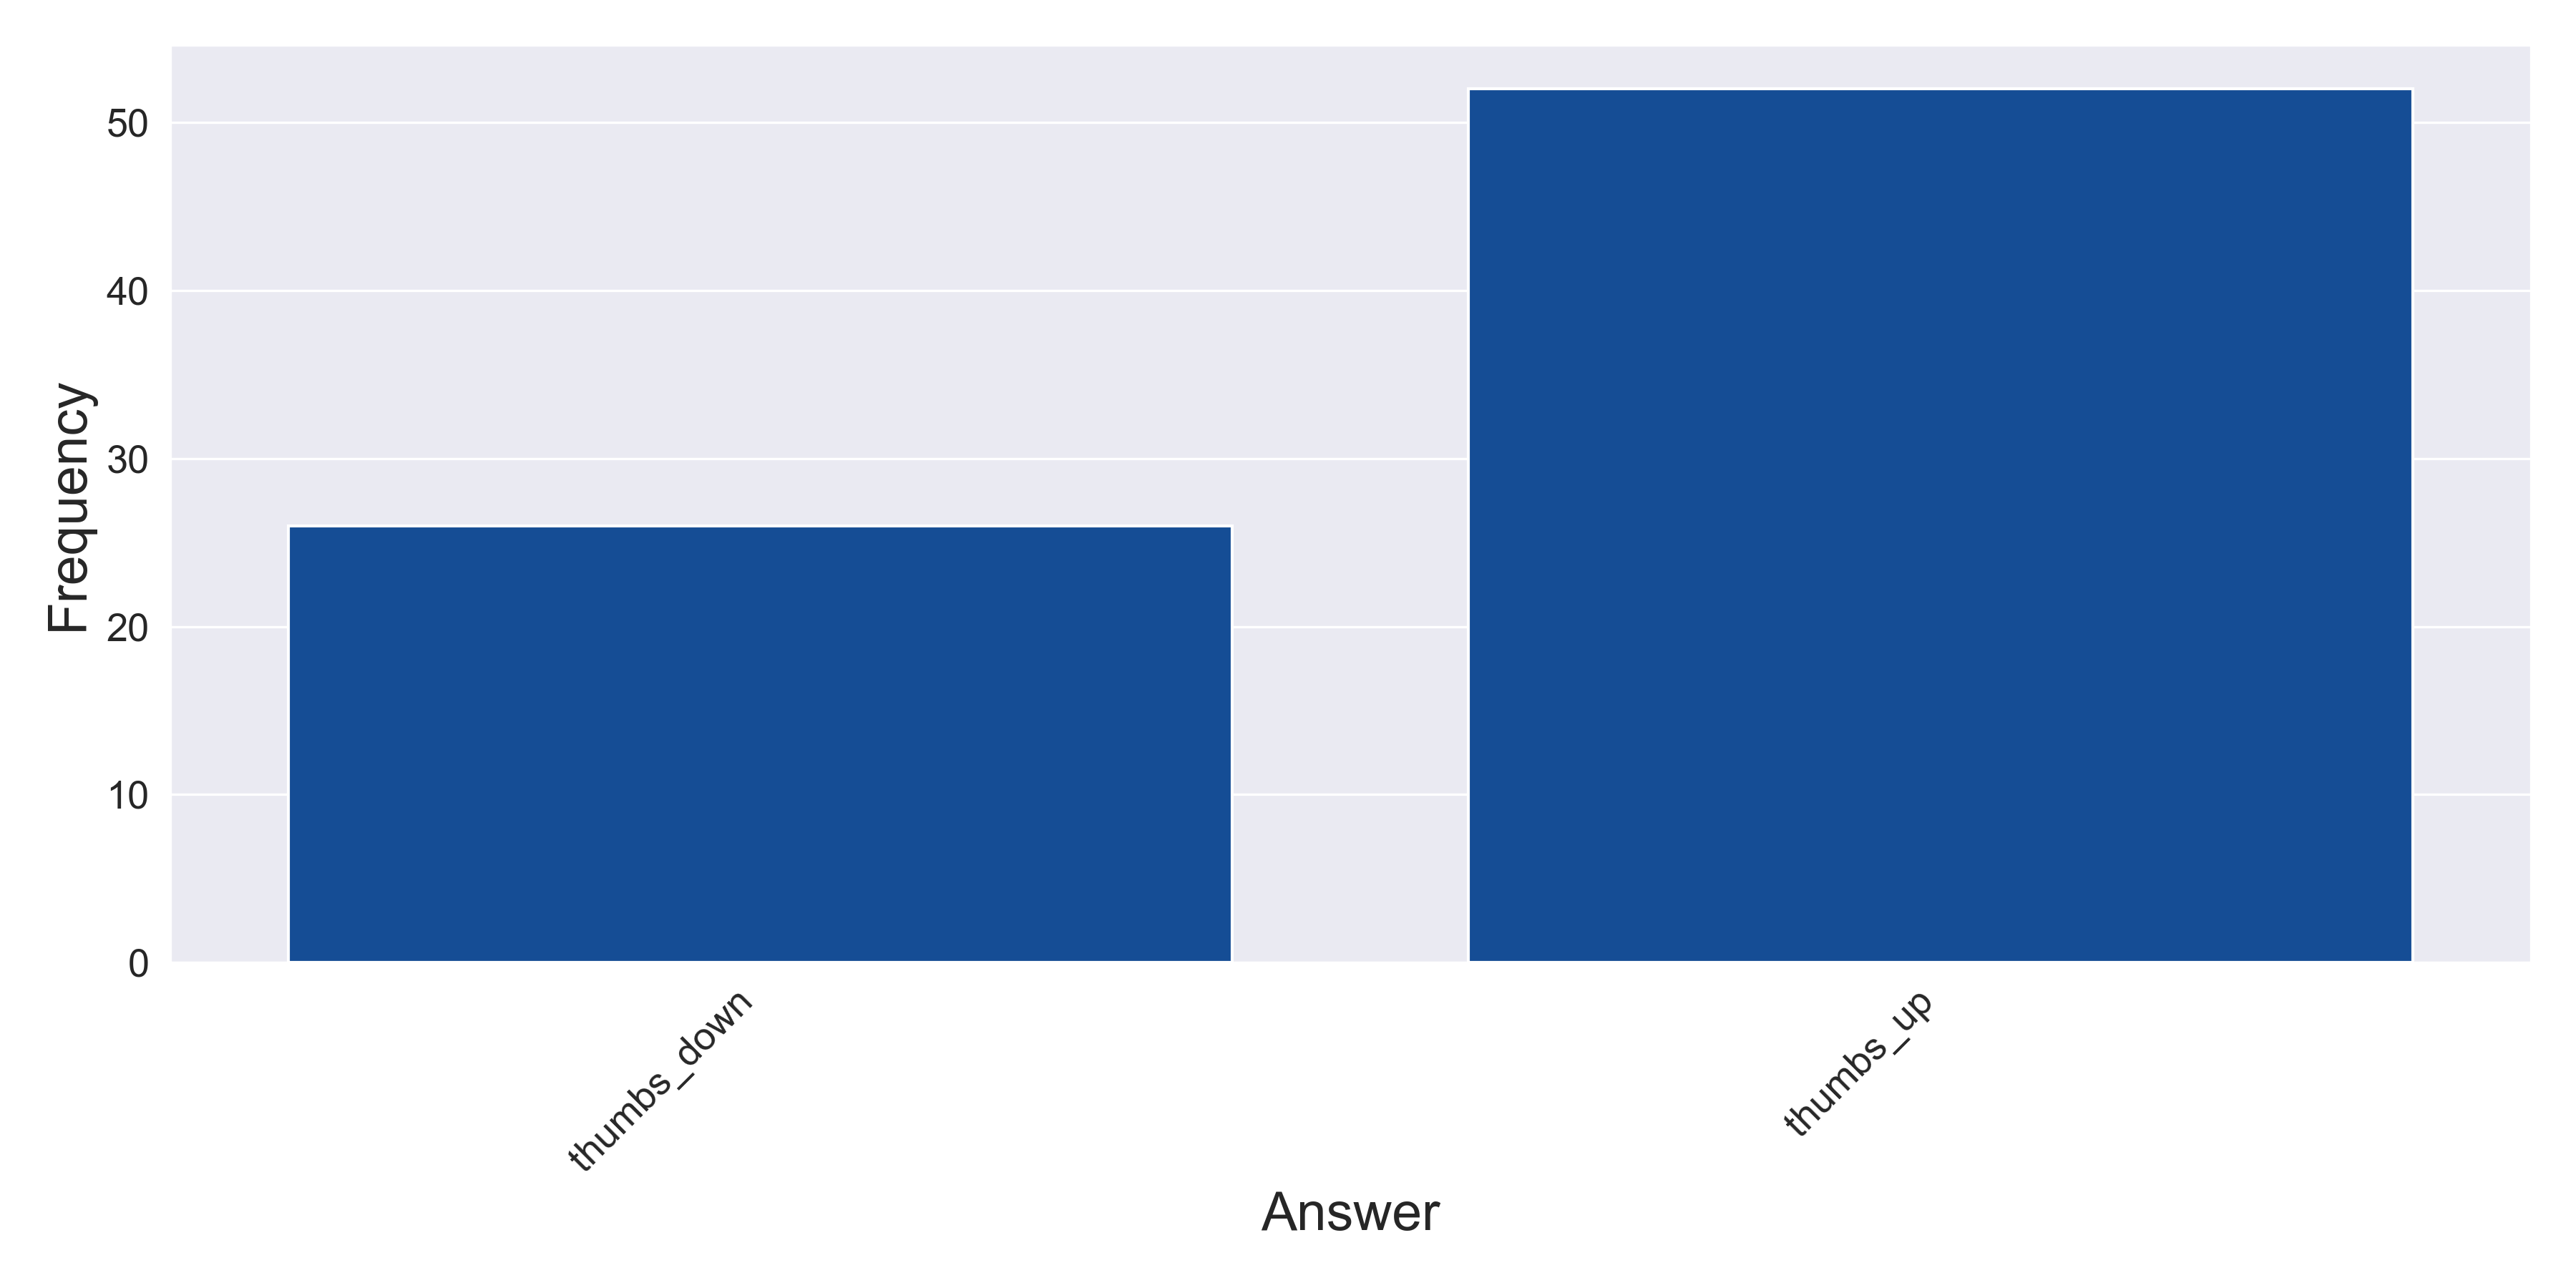
\includegraphics[width=1\textwidth]{results/plots/assets/feedback-01-frequency-of-answer-for-question-2e09fd.png}
    \caption{The number of answers to each answer for the question \textit{"Was this a good reply?"}}
    \label{fig:feedback_01_frequency_of_answer_for_question_2e09fd}
\end{figure}


\begin{figure}[H]
    \centering
    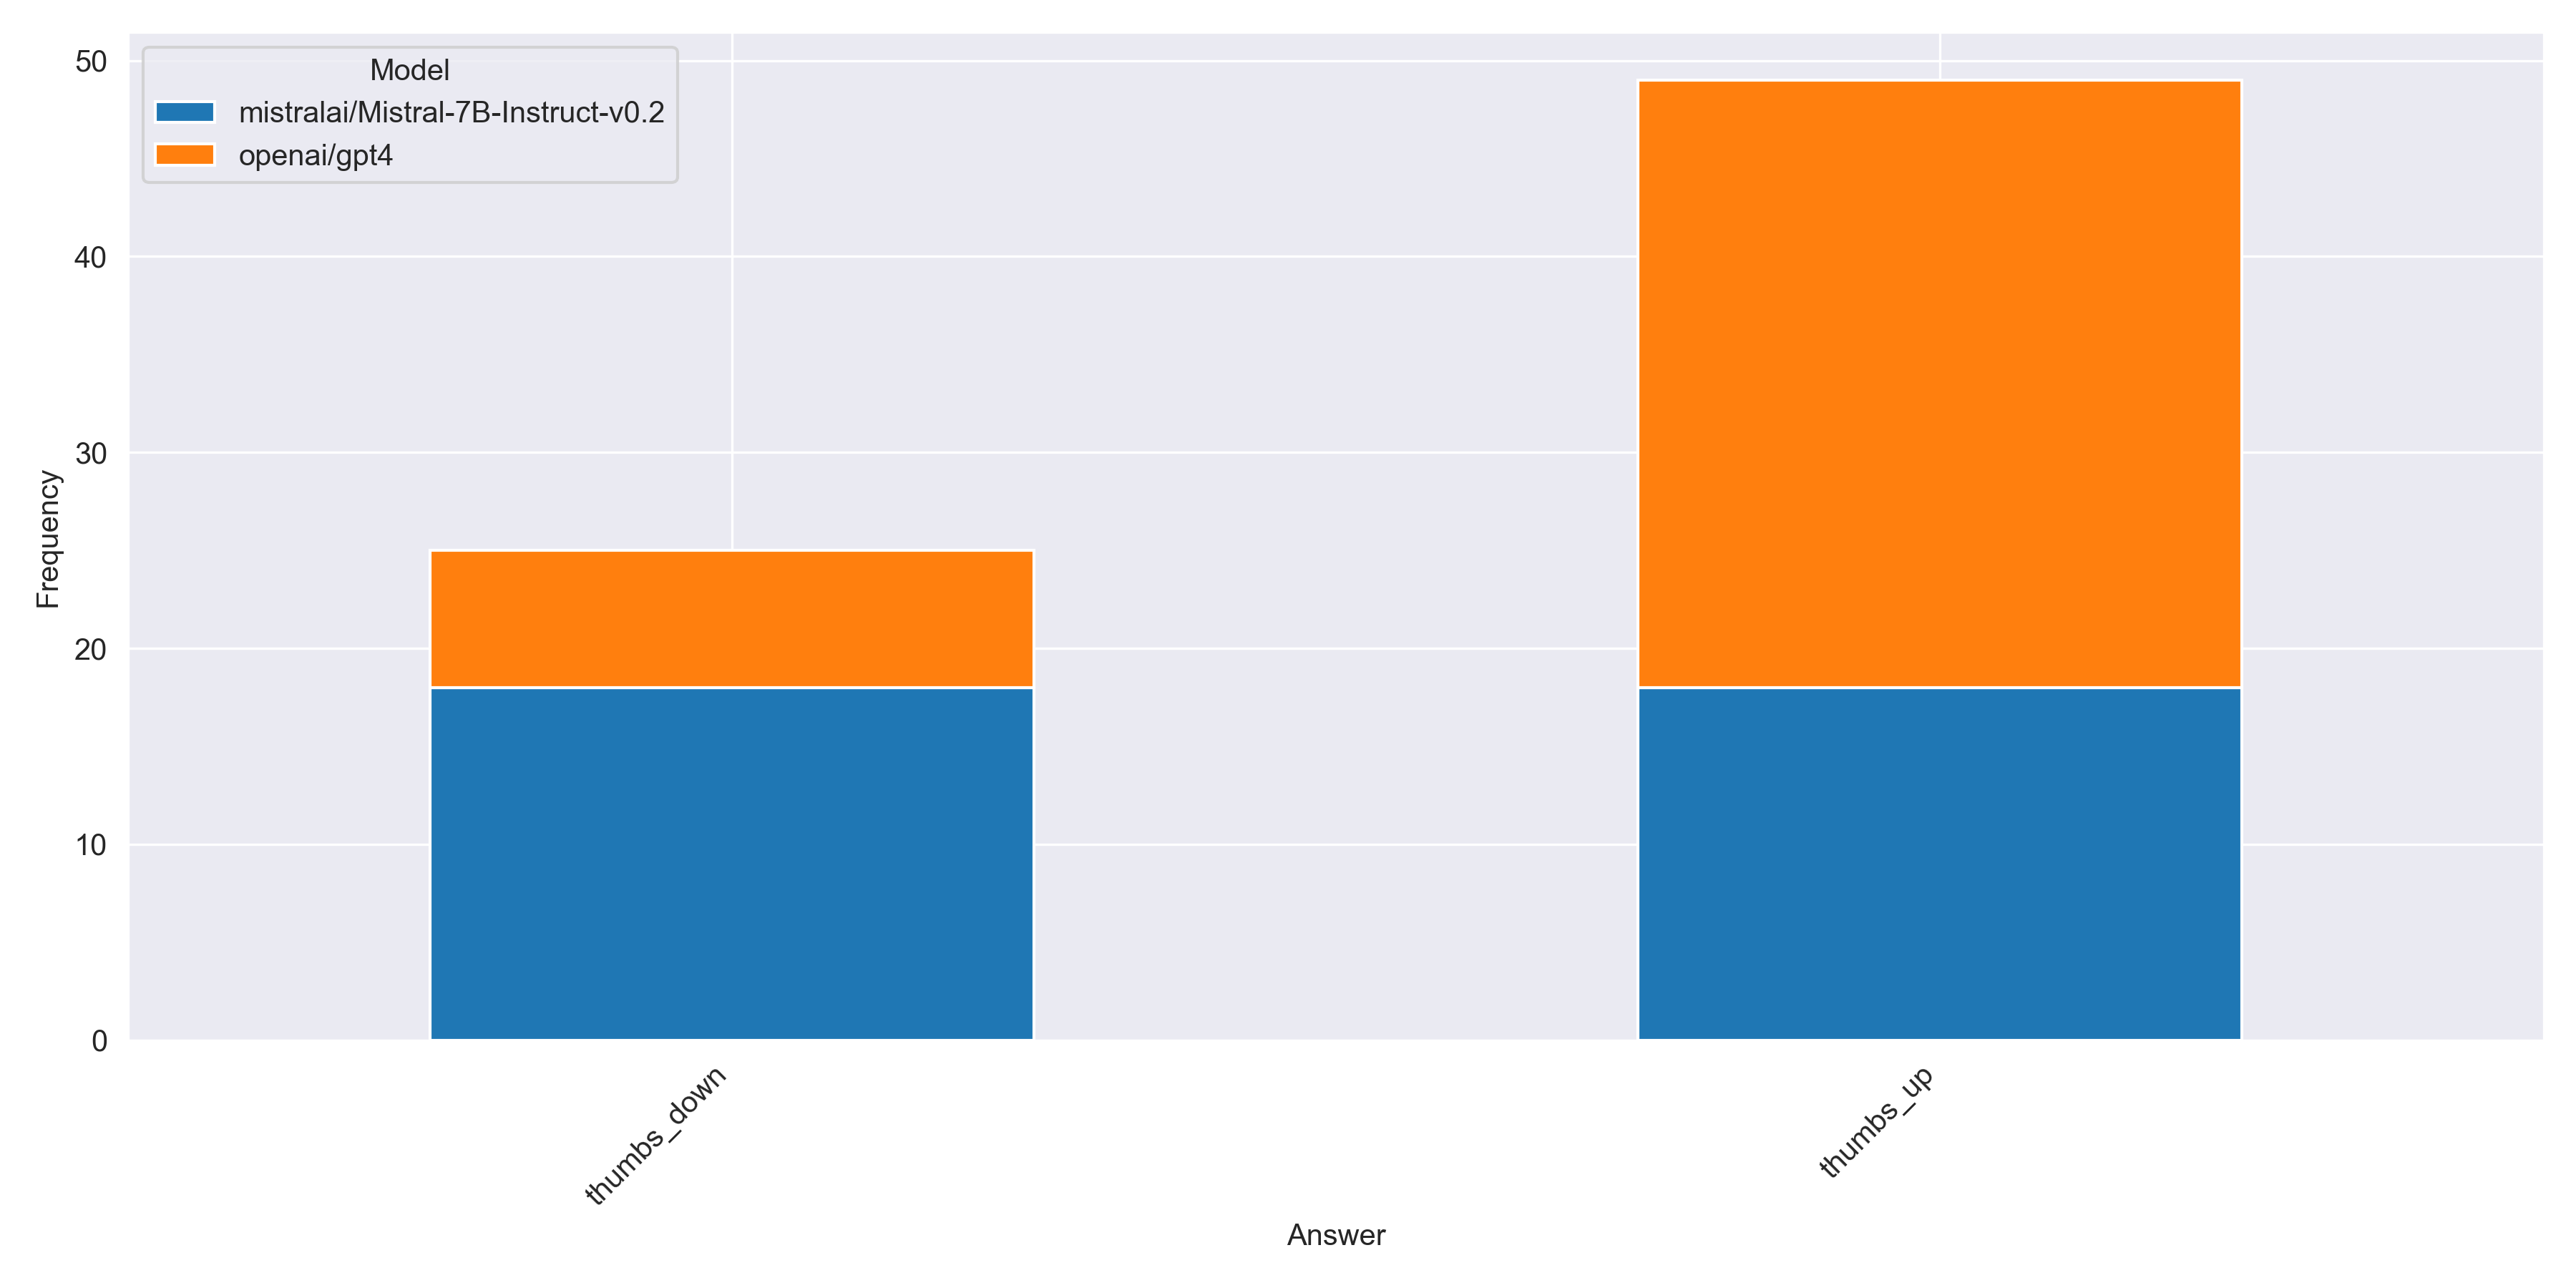
\includegraphics[width=\textwidth]{results/plots/assets/feedback-02-frequency-of-answer-for-question-per-model-2e09fd.png}
    \caption{The number of answers to each answer for the question \textit{"Was this a good reply?"}}
    \label{fig:feedback_02_frequency_of_answer_for_question_per_model_2e09fd}
\end{figure}


\subsection{Survey questions injected into the chat}


The software written for this thesis was, as discussed in sections \ref{sec:method_feedback_data} and \ref{sec:what_you_did_gathering_feedback_data}, and shown in \autoref{fig:multiple_choice}, designed to gather user feedback by injecting questions in the chat at certain triggers. The questions inserted after receiving the first response in chat number 2, 4 and 6 of each session can be seen in table x. The questions inserted after receiving the first response in chat number 8 can be seen in table y.


Unfortunately, very few of the users who used the system answered these questions. Table z shows how many answers the first set of questions got, and how many answers the second set of questions got.


However, for the users that did answer the first set of questions, their answers can be seen in figures \ref{fig:feedback_01_frequency_of_answer_for_question_cbfea1}, \ref{fig:feedback_01_frequency_of_answer_for_question_ead094} and \ref{fig:feedback_01_frequency_of_answer_for_question_d474ac}.


\begin{figure}[H]
    \centering
    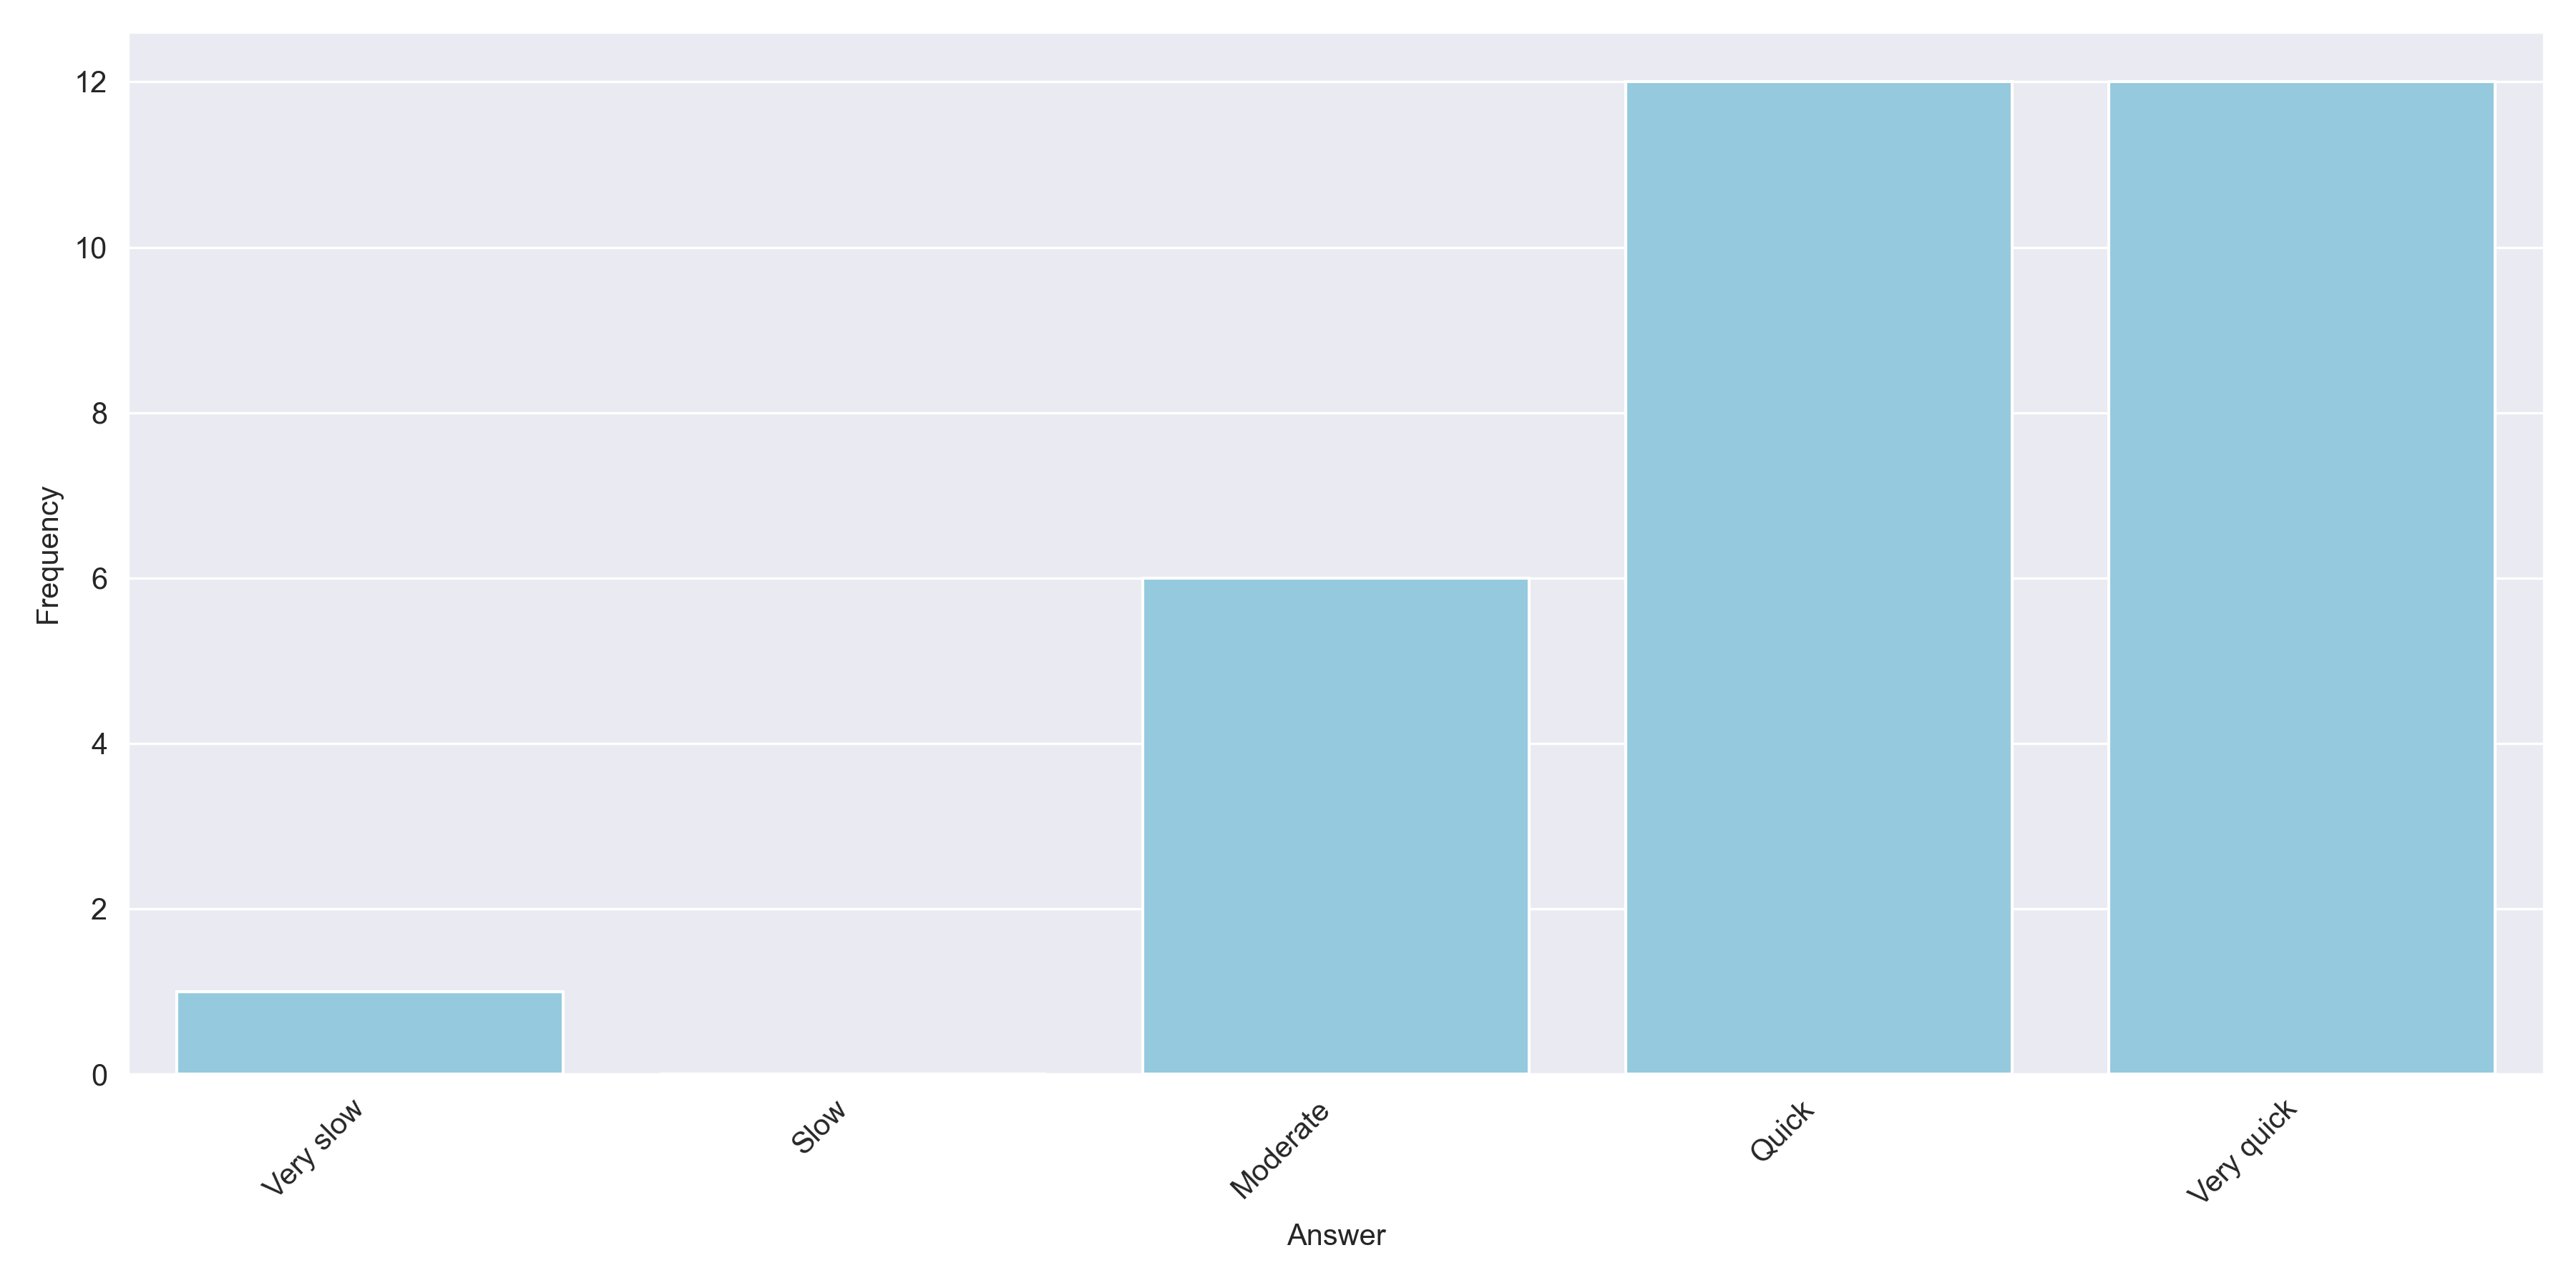
\includegraphics[width=1\textwidth]{results/plots/assets/feedback-01-frequency-of-answer-for-question-cbfea1.png}
    \caption{The number of answers to each answer for the question \textit{"How would you rate the speed of the bot's reply?"}}
    \label{fig:feedback_01_frequency_of_answer_for_question_cbfea1}
\end{figure}


\begin{figure}[H]
    \centering
    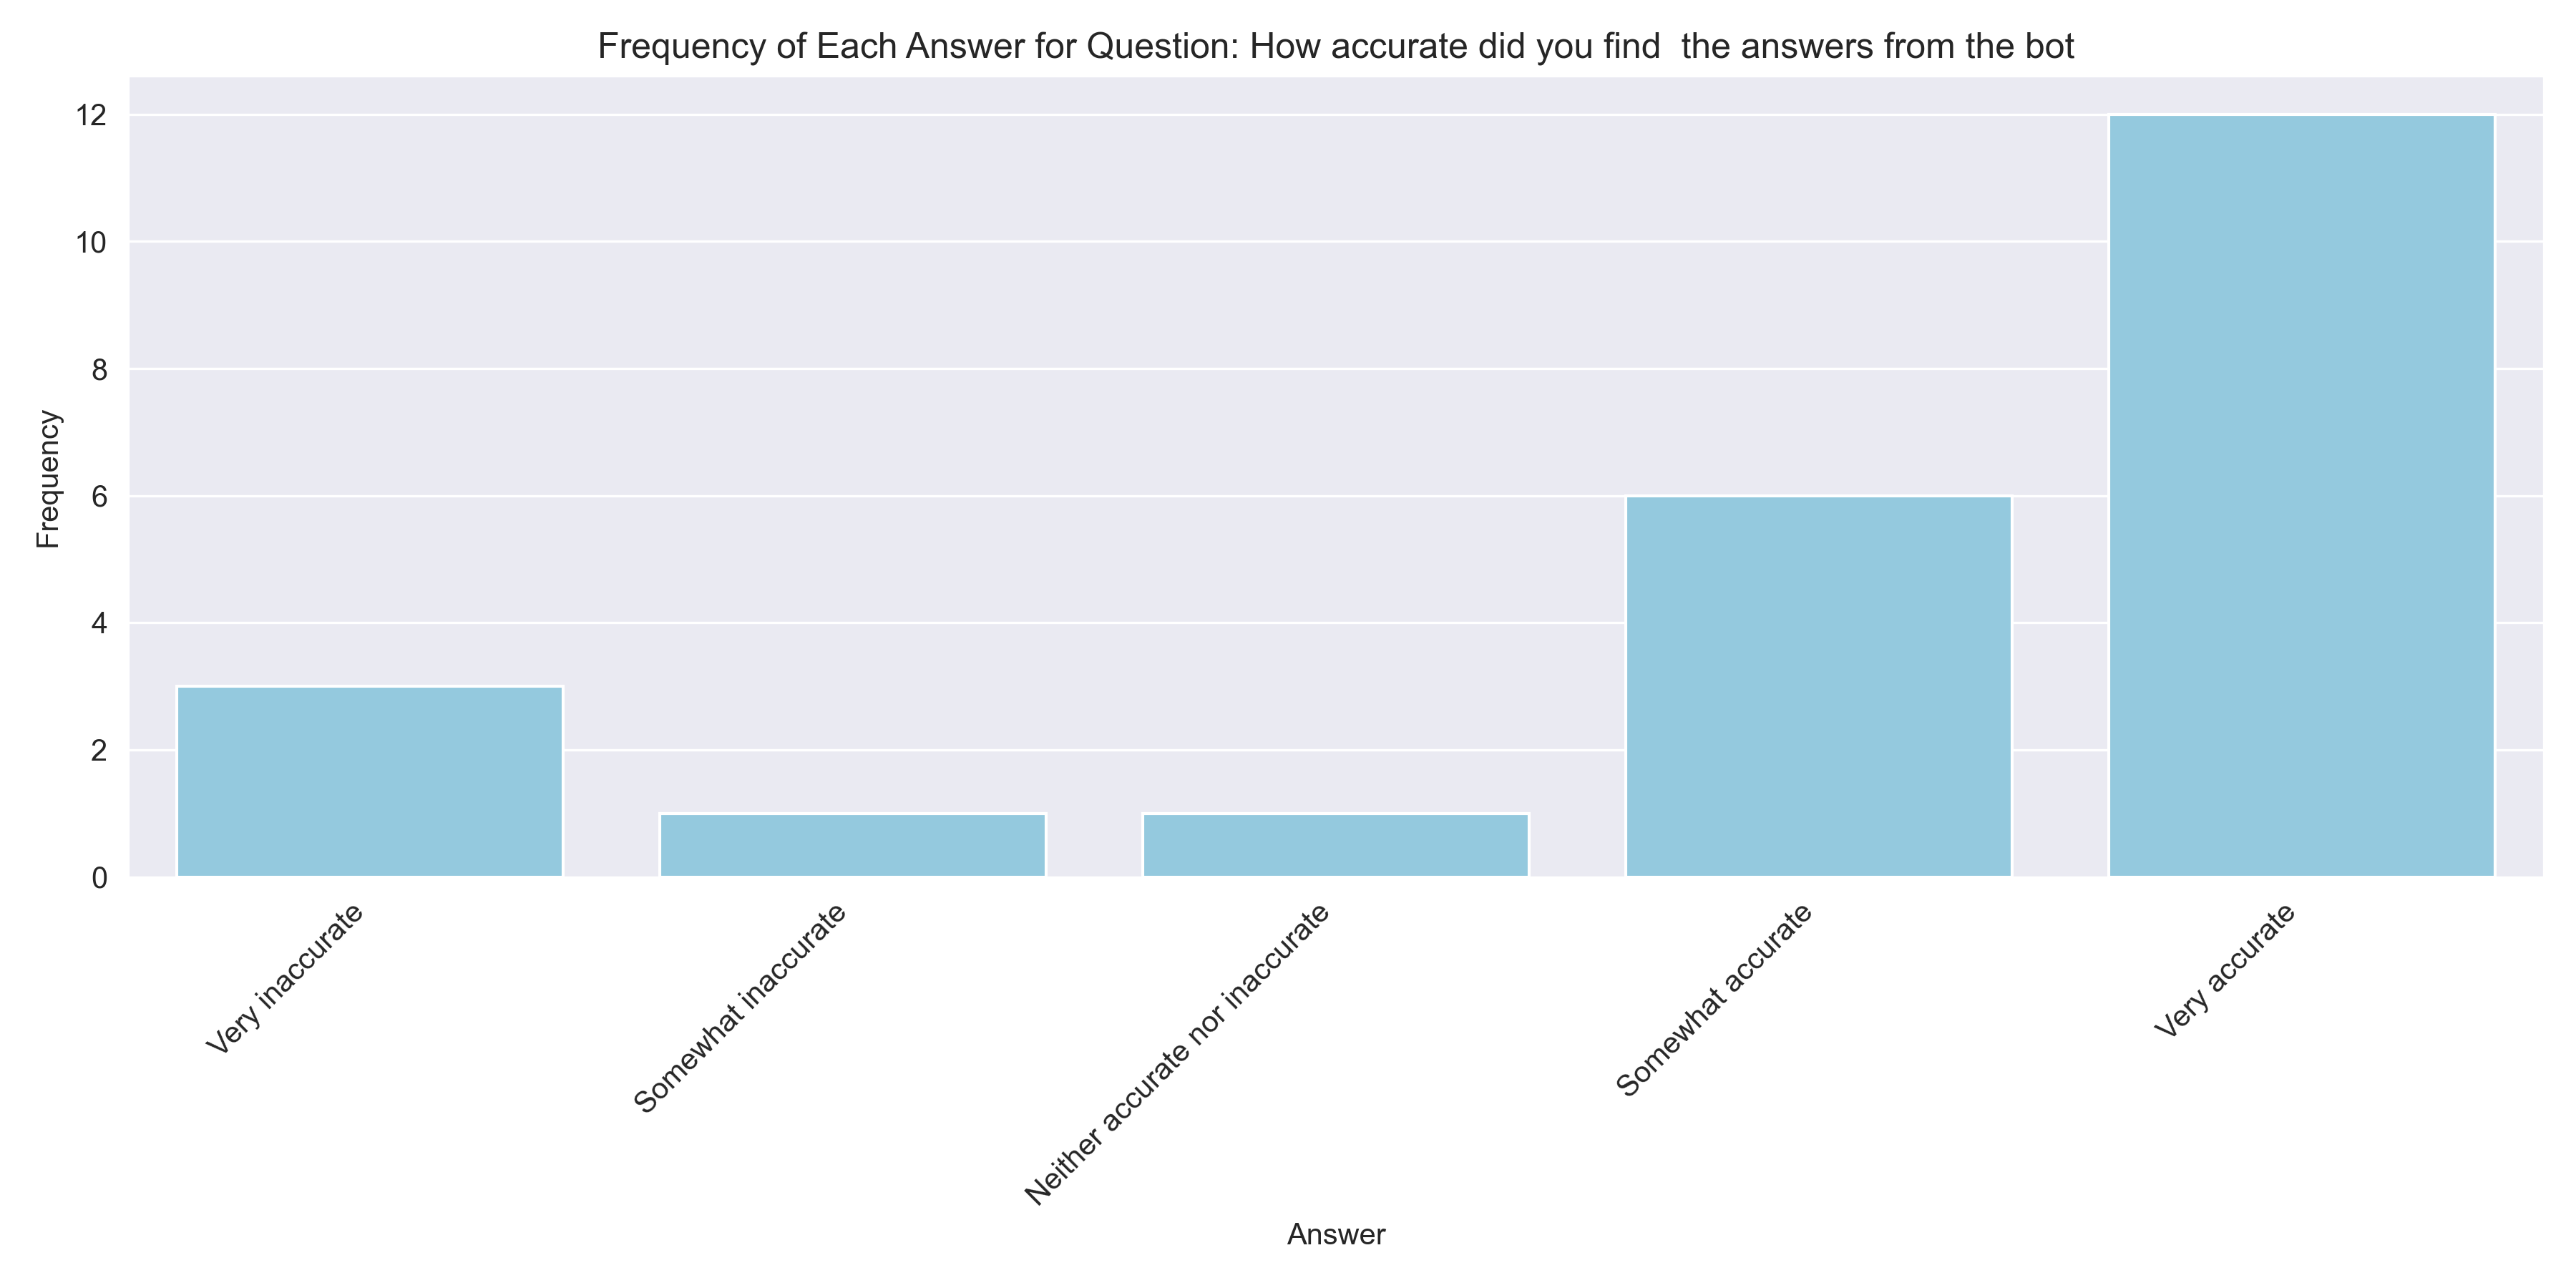
\includegraphics[width=\textwidth]{results/plots/assets/feedback-01-frequency-of-answer-for-question-ead094.png}
    \caption{The number of answers to each answer for the question \textit{"How accurate did you find  the answers from the bot"}}
    \label{fig:feedback_01_frequency_of_answer_for_question_ead094}
\end{figure}


\begin{figure}[H]
    \centering
    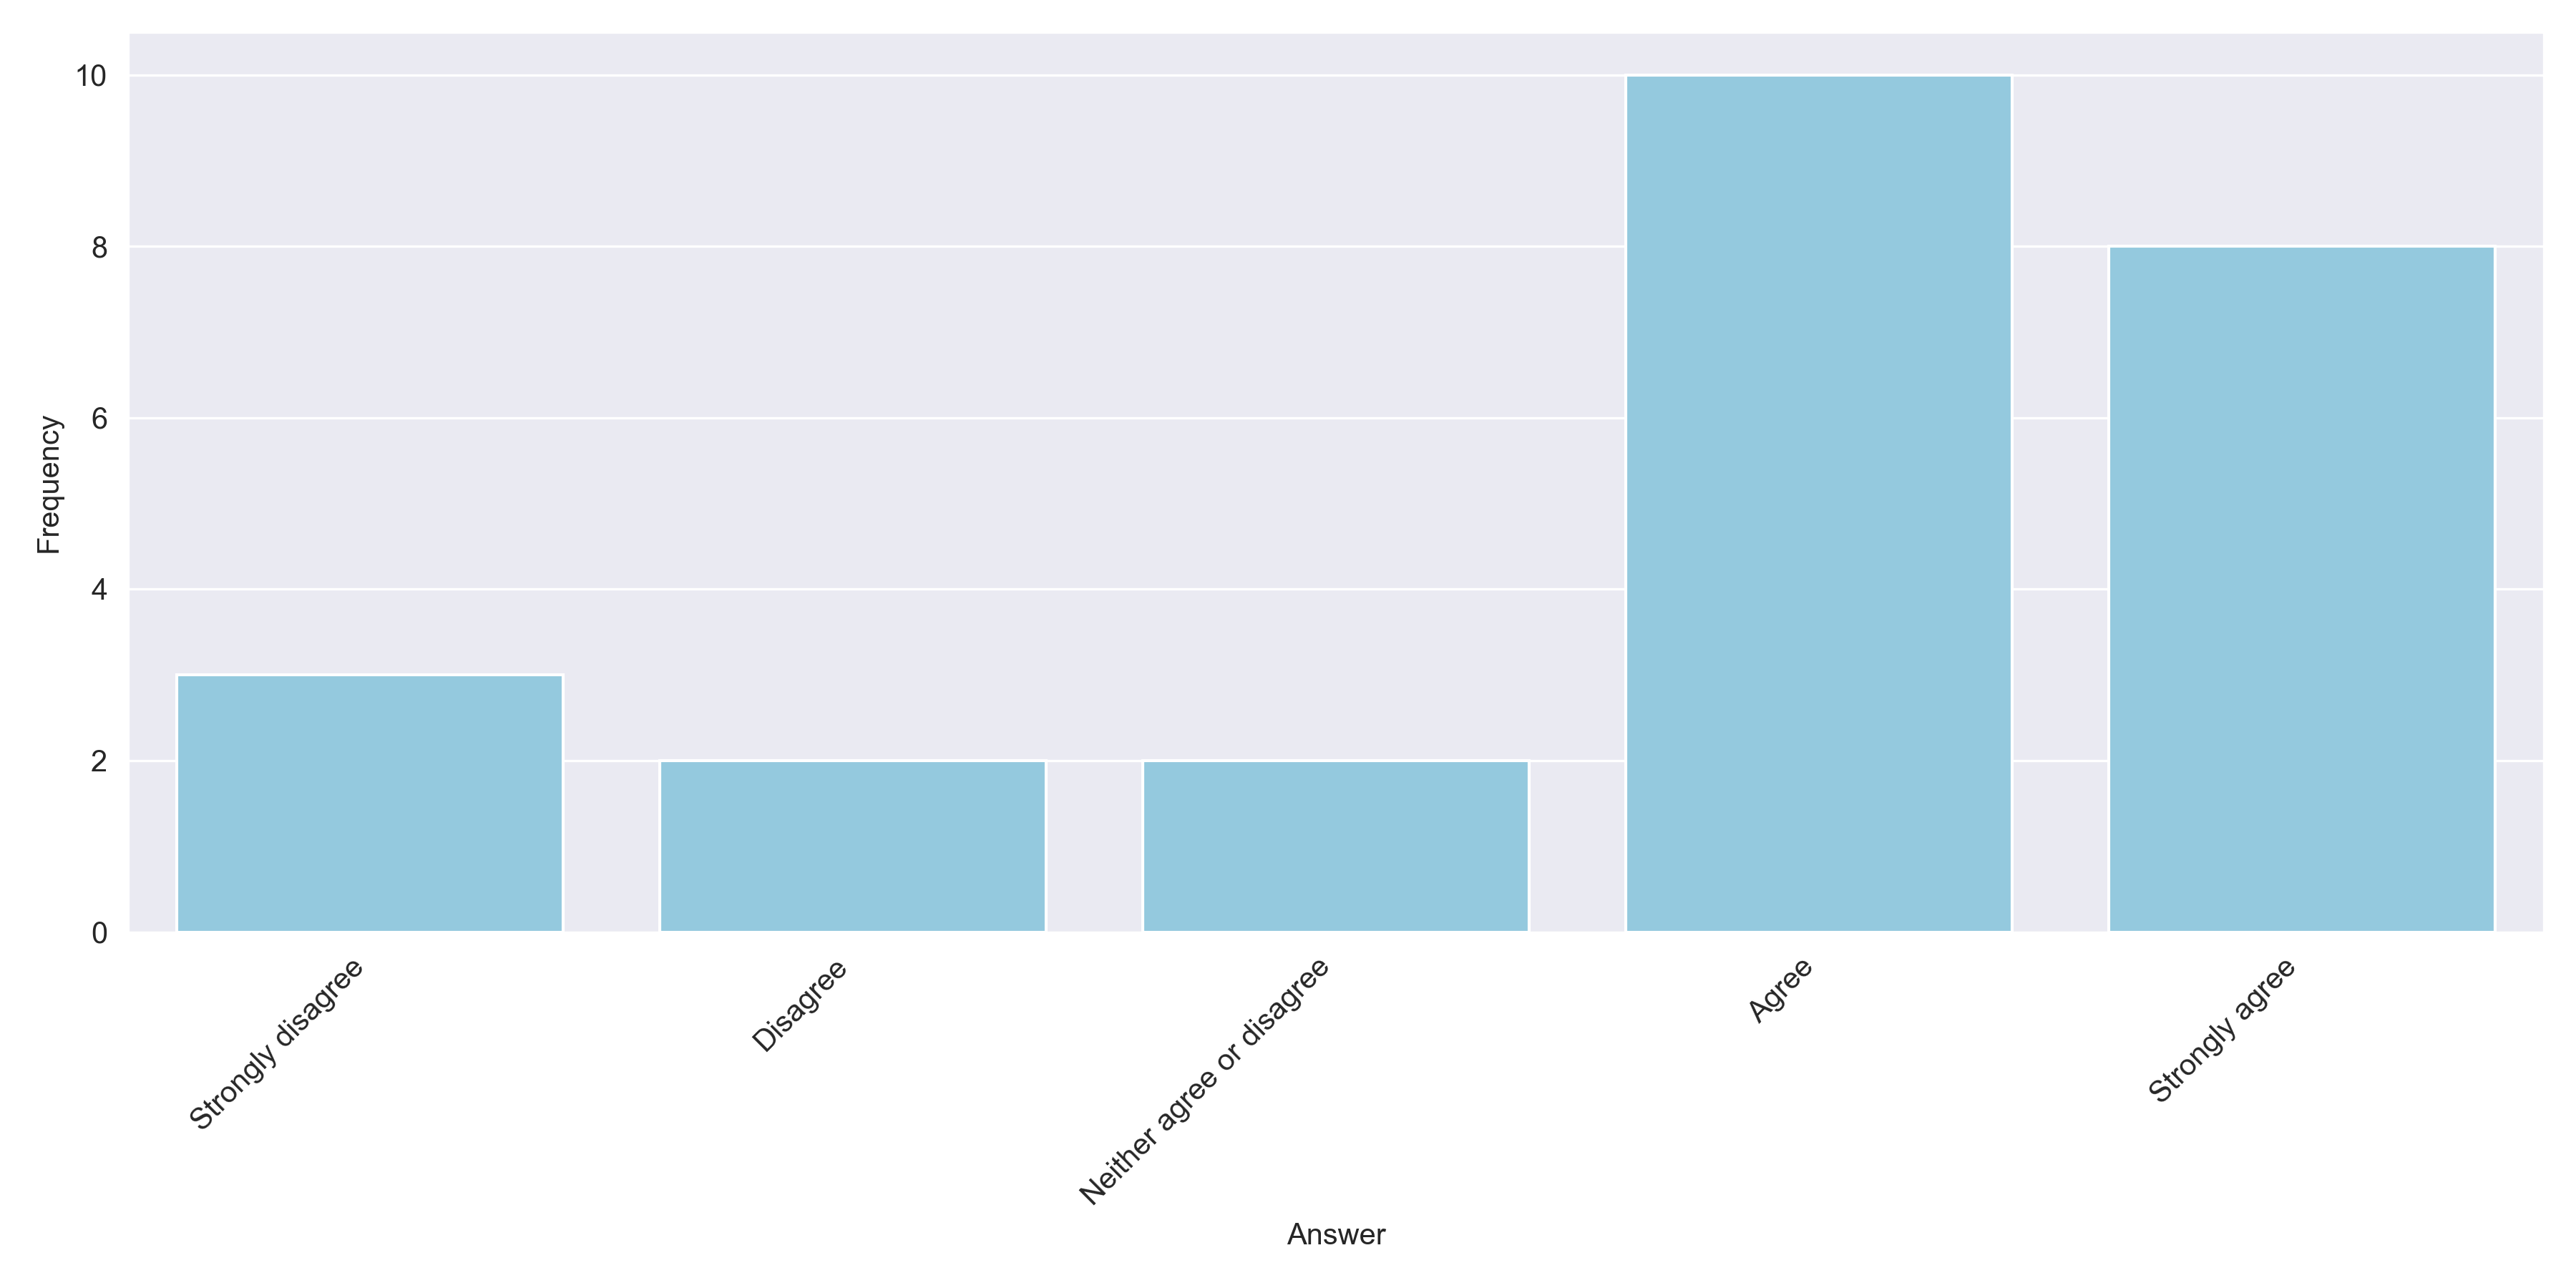
\includegraphics[width=1\textwidth]{results/plots/assets/feedback-01-frequency-of-answer-for-question-d474ac.png}
    \caption{The number of answers to each answer for the question \textit{"The reply from the bot was useful to me"}}
    \label{fig:feedback_01_frequency_of_answer_for_question_d474ac}
\end{figure}


Since the number of answers weren't many, the study couldn’t sample between more than two different configurations. These two configurations used different \gls{LLM}s, but shared the same retrieval strategy (vector search) and embedding function (\textit{openai/text-embedding-3-large}). In figures \ref{fig:feedback_02_frequency_of_answer_for_question_per_model_cbfea1}, \ref{fig:feedback_02_frequency_of_answer_for_question_per_model_ead094} and \ref{fig:feedback_02_frequency_of_answer_for_question_per_model_d474ac} how users that were assigned the different \gls{LLM}s answered can be seen.


\begin{figure}[H]
    \centering
    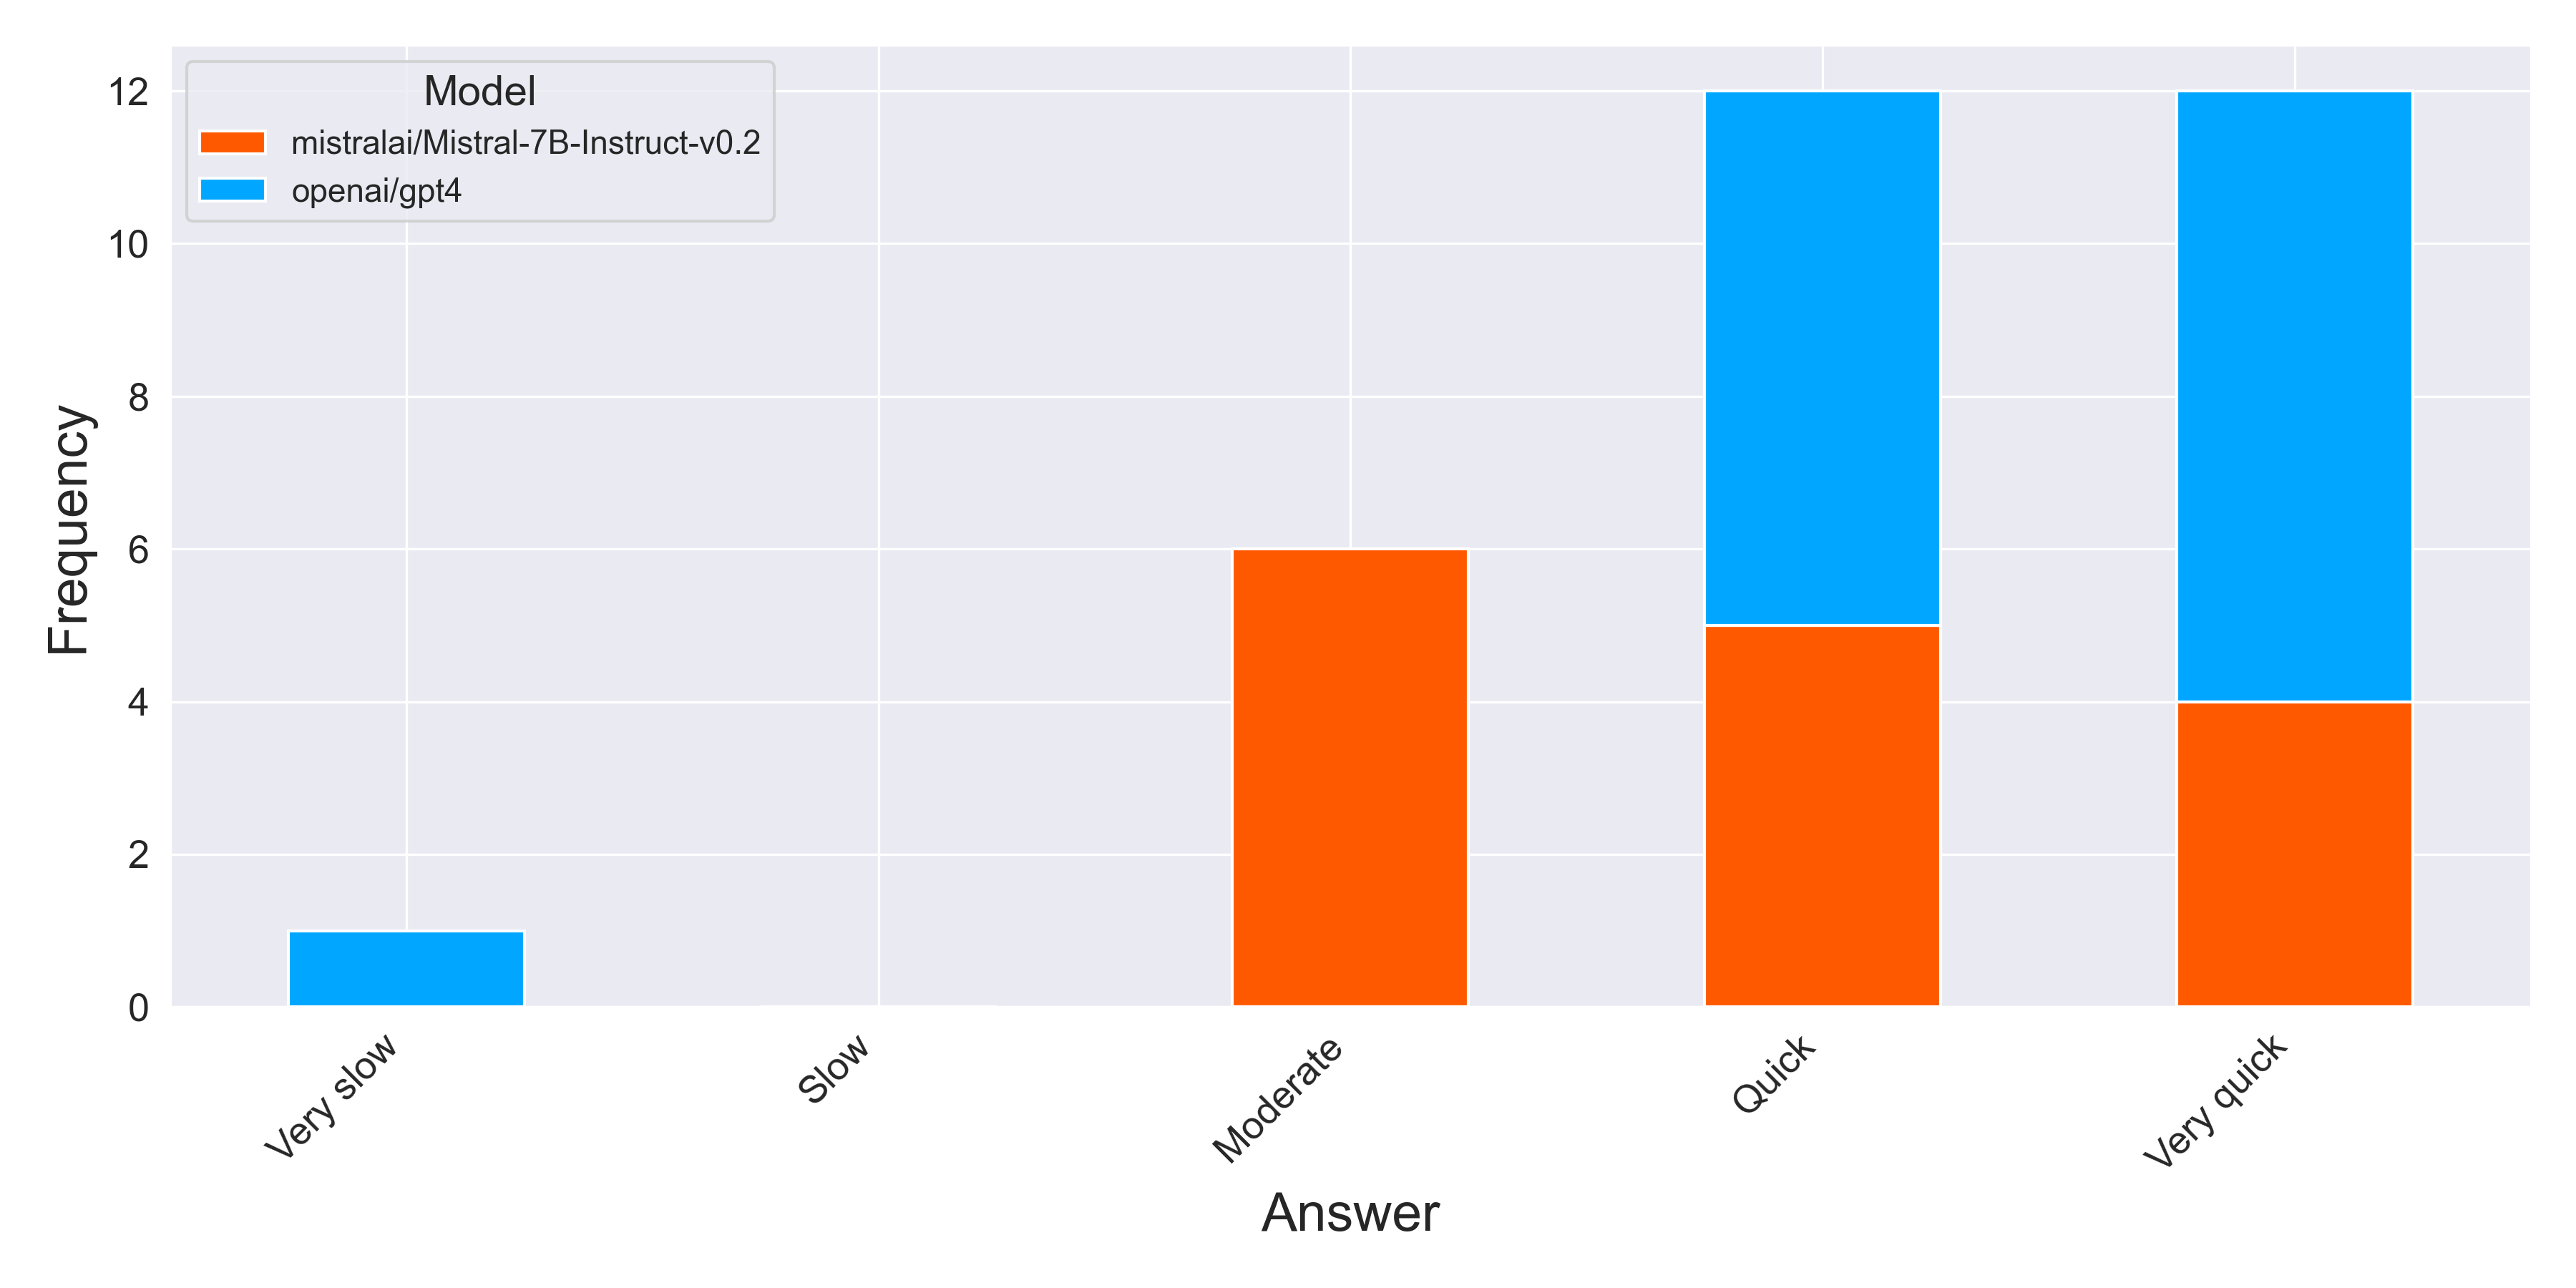
\includegraphics[width=1\textwidth]{results/plots/assets/feedback-02-frequency-of-answer-for-question-per-model-cbfea1.png}
    \caption{The number of answers to each answer for the question \textit{"How would you rate the speed of the bot's reply?"}}
    \label{fig:feedback_02_frequency_of_answer_for_question_per_model_cbfea1}
\end{figure}


\begin{figure}[H]
    \centering
    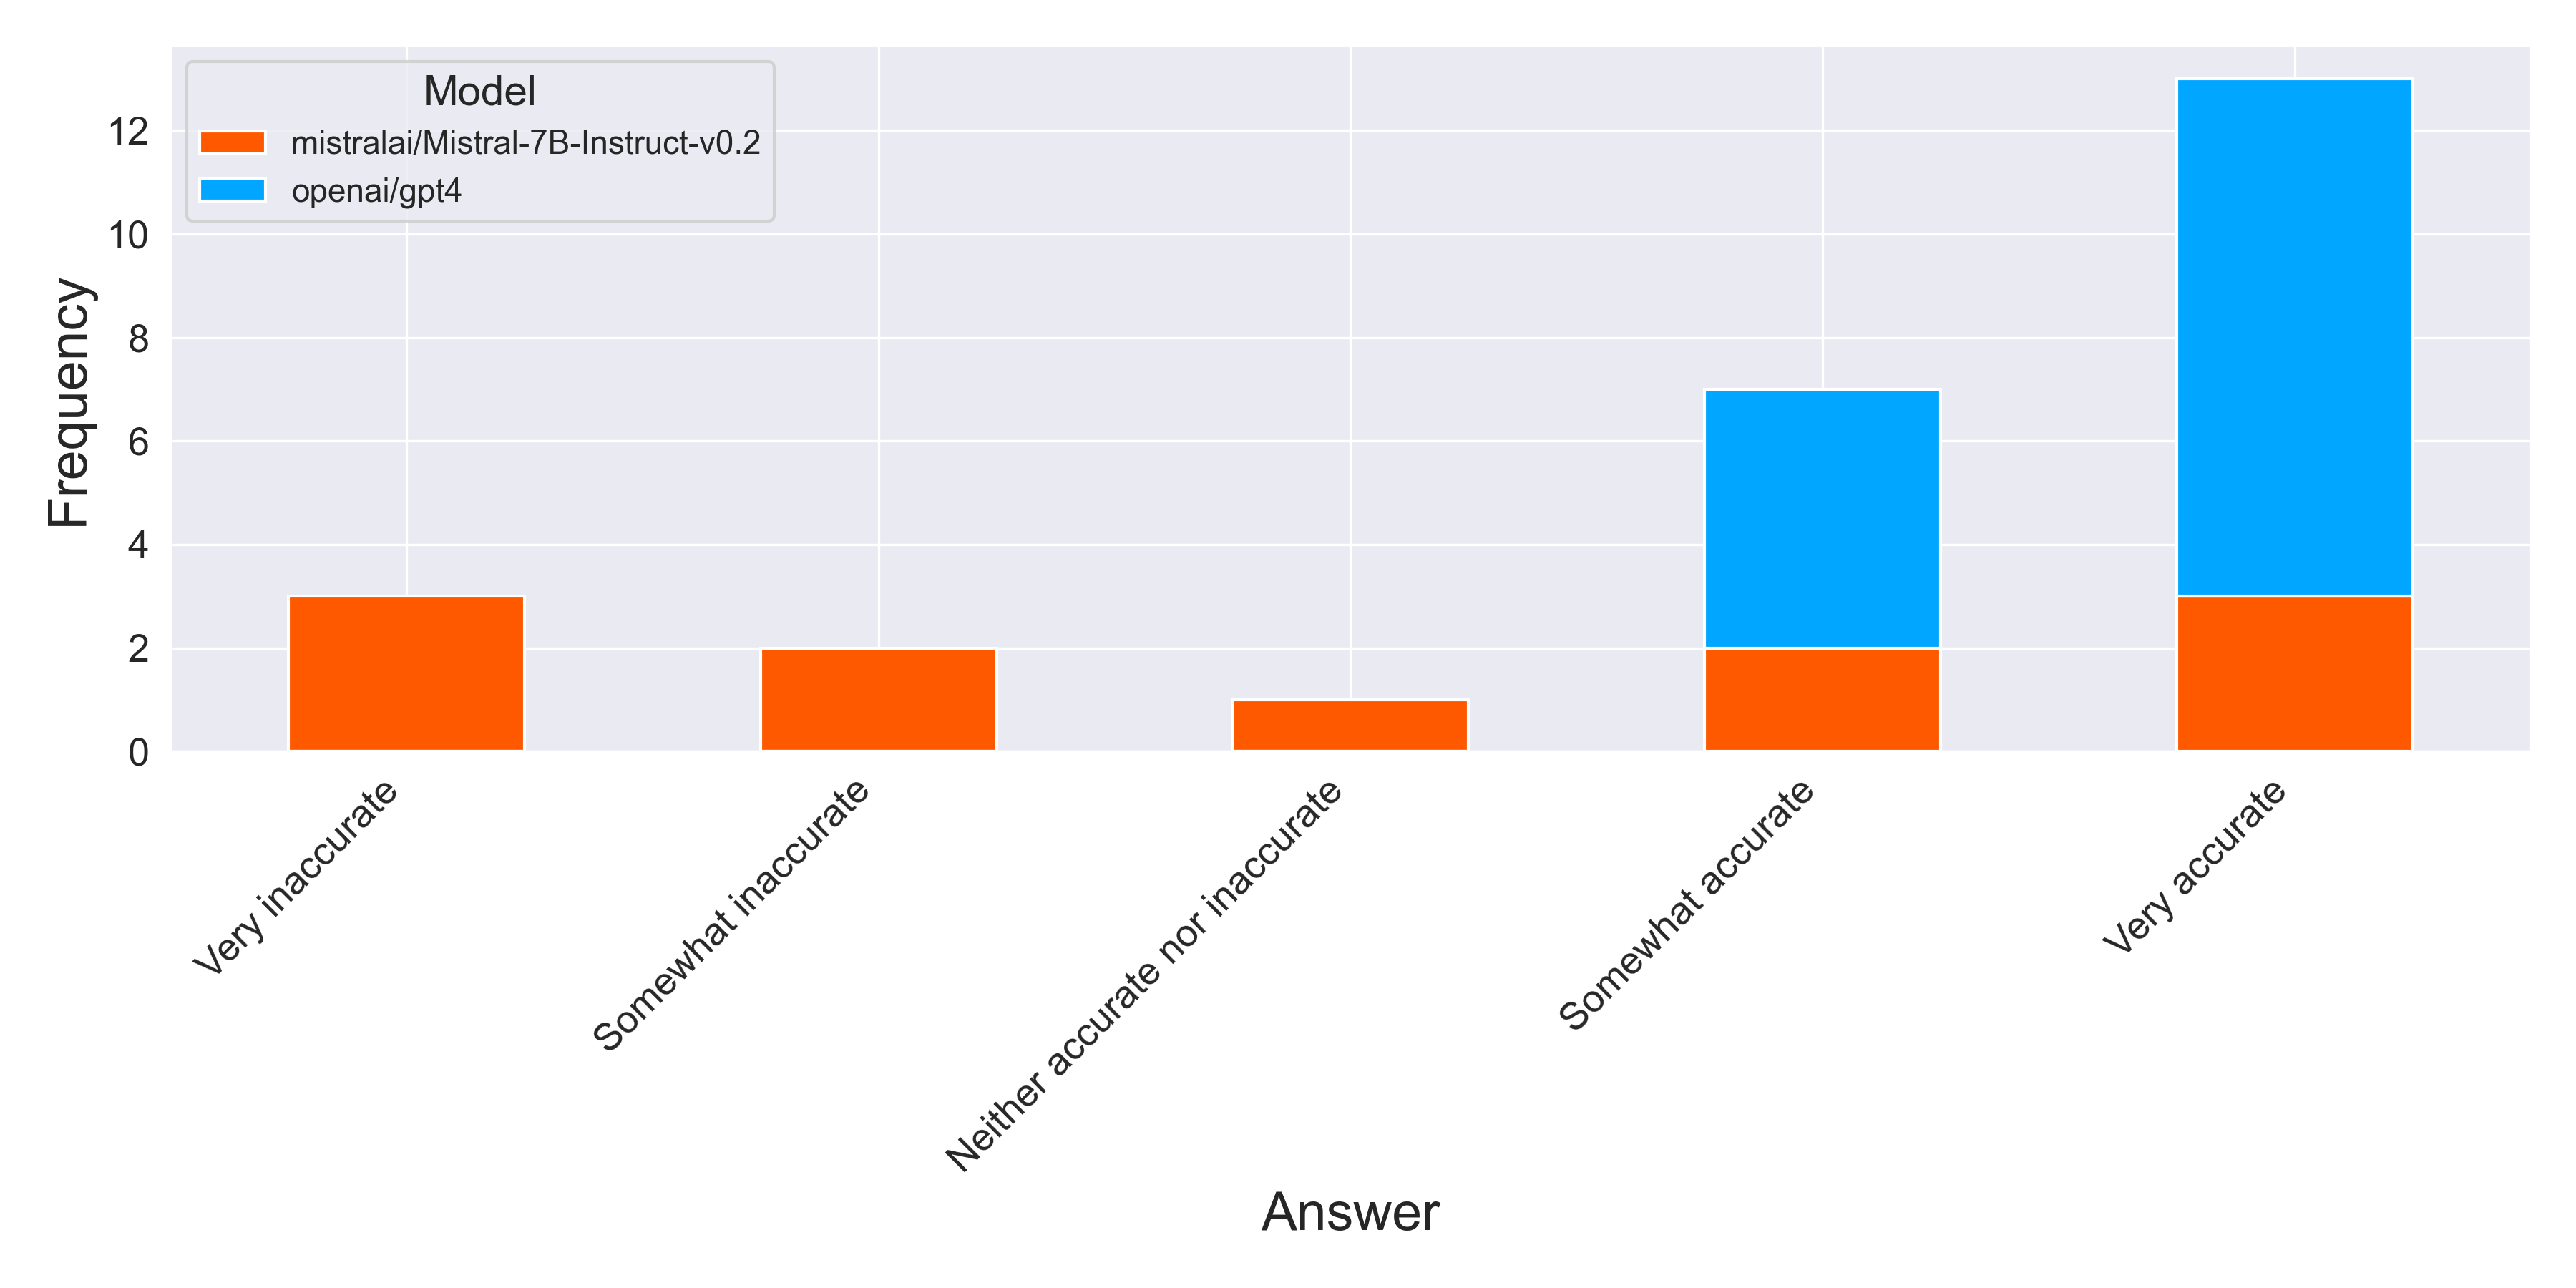
\includegraphics[width=1\textwidth]{results/plots/assets/feedback-02-frequency-of-answer-for-question-per-model-ead094.png}
    \caption{The number of answers to each answer for the question \textit{"How accurate did you find  the answers from the bot"}}
    \label{fig:feedback_02_frequency_of_answer_for_question_per_model_ead094}
\end{figure}


\begin{figure}[H]
    \centering
    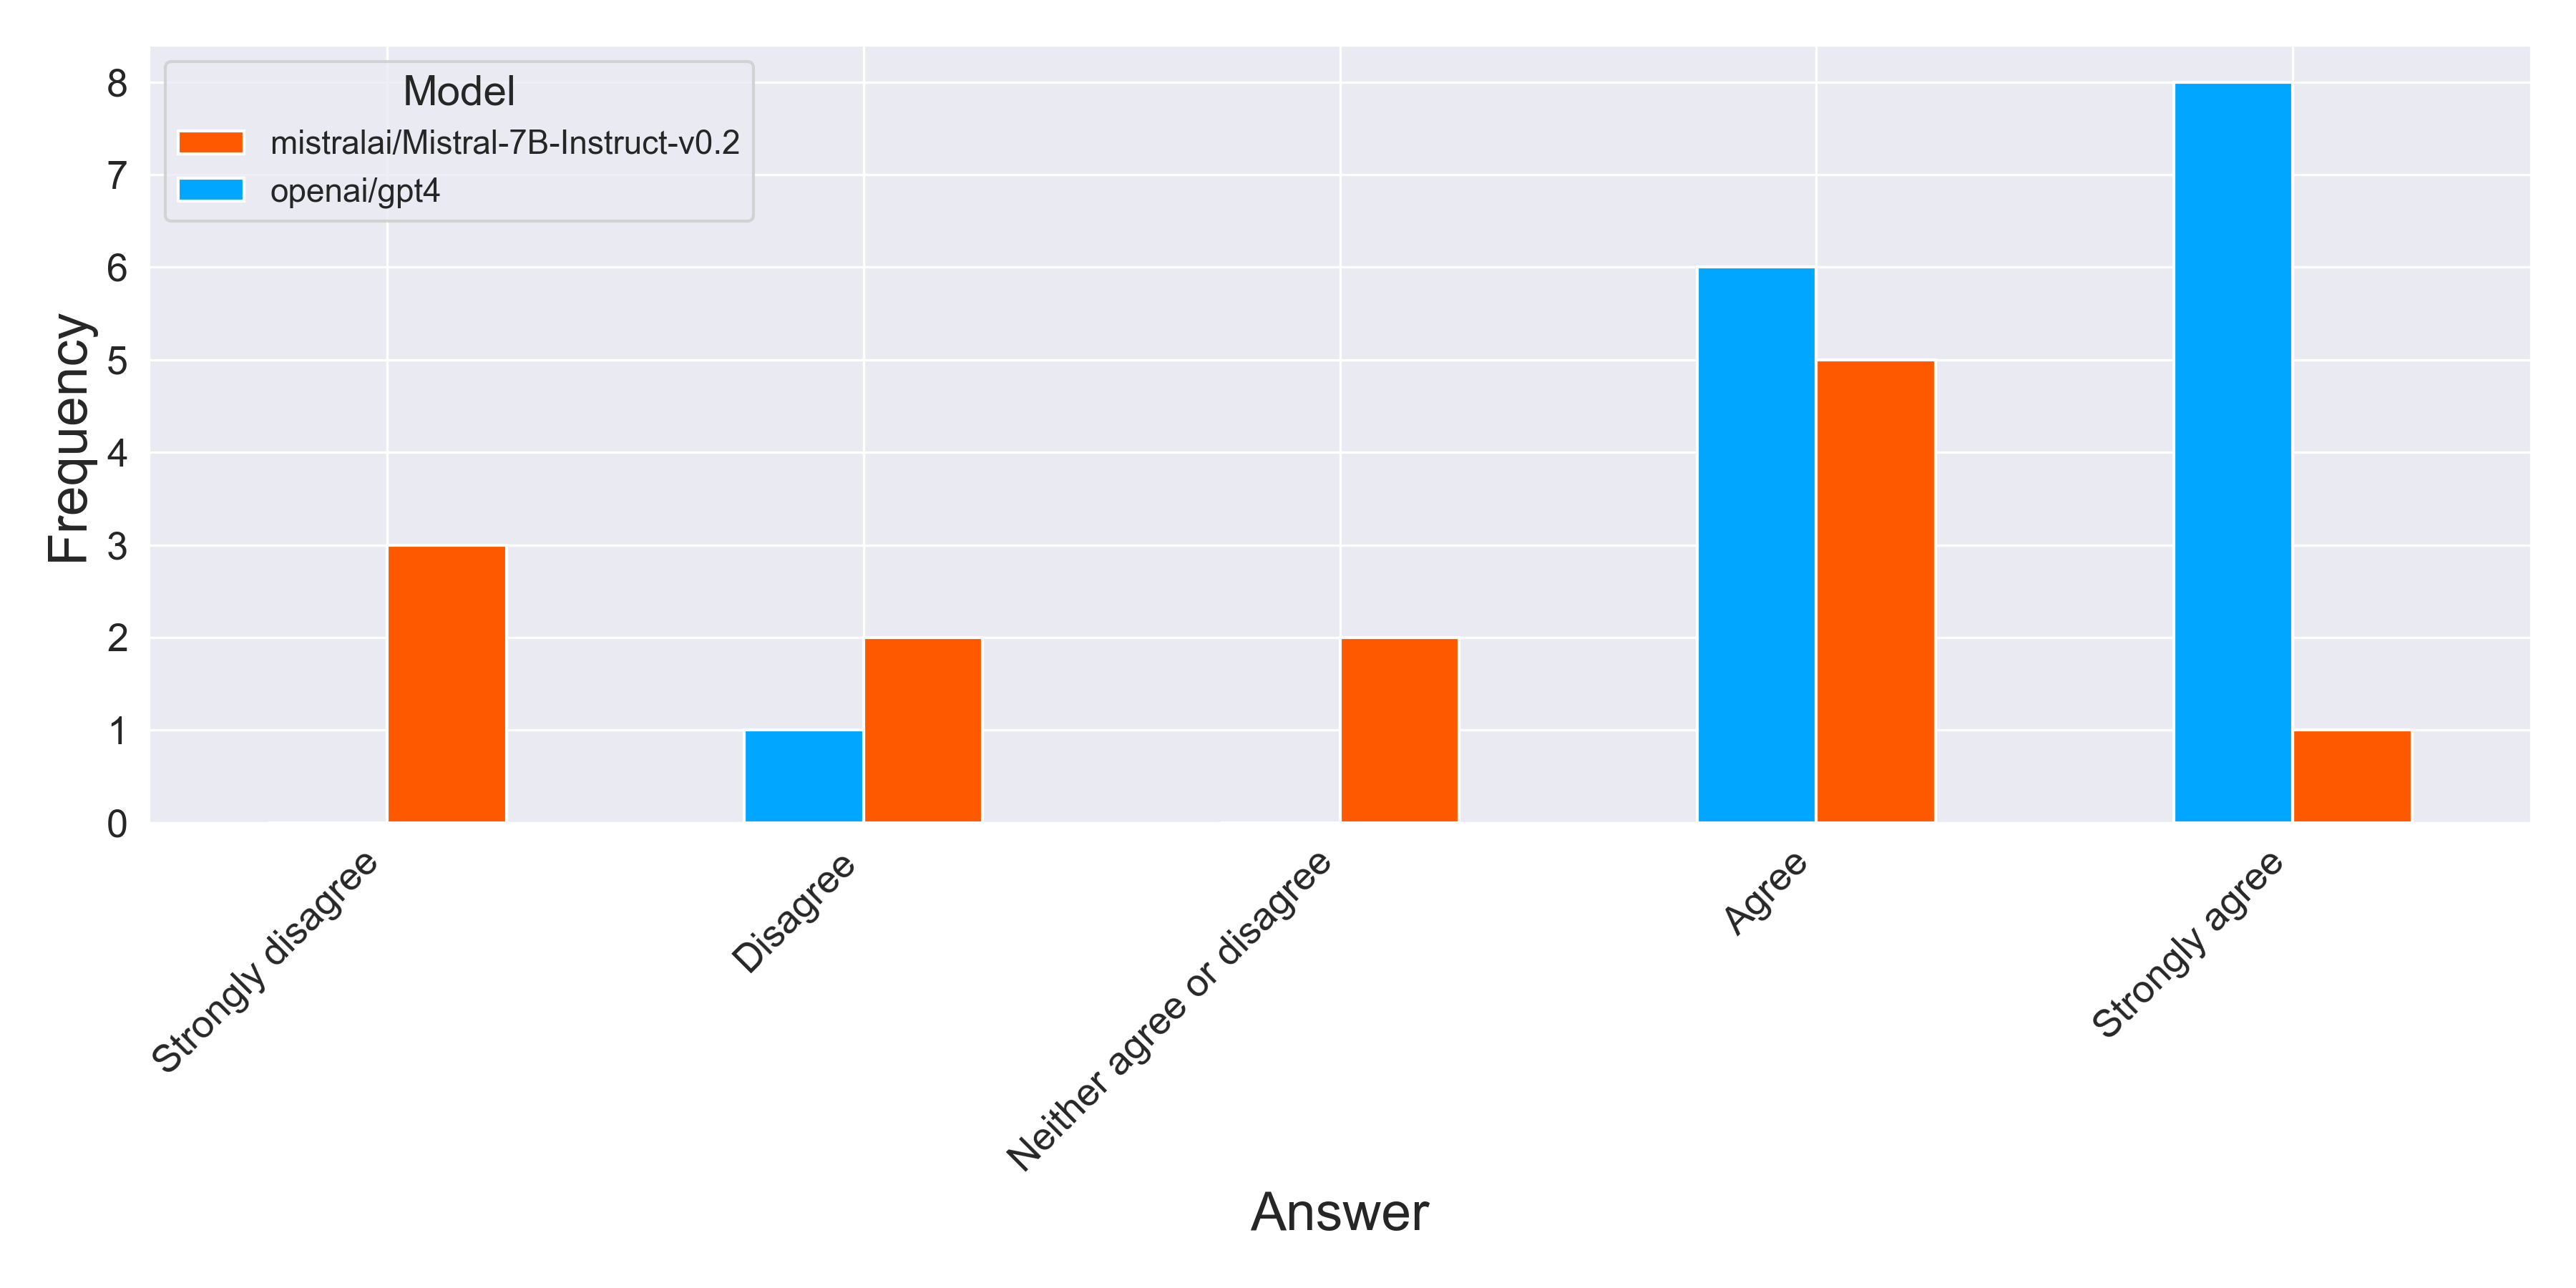
\includegraphics[width=\textwidth]{results/plots/assets/feedback-02-frequency-of-answer-for-question-per-model-d474ac.png}
    \caption{The number of answers to each answer for the question \textit{"The reply from the bot was useful to me"}}
    \label{fig:feedback_02_frequency_of_answer_for_question_per_model_d474ac}
\end{figure}


\subsection{Form submitted at the end of the course}




\section{Qualitative analysis of user responses}
\label{sec:qualitative_analysis_of_user_responses}


This section will present an analysis of the free text answers users have provided in the forms that have been presented in the participating courses.




% \sweExpl{Lite statistik av fördröjningsmätningarna visas i Tabell~\ref{tab:delayMeasurements}. Förseningen har beräknats från den tidpunkt då begäran GET tas emot fram till svaret skickas.}


\section{Reliability Analysis}


% \sweExpl{Analys av tillförlitlighet\\
% Tillförlitlighet i metod och data}


\section{Validity Analysis}


% \sweExpl{Analys av validitet\\
% Validitet i metod och data}


\cleardoublepage